\chapter{方程和优化}
\label{chap:linear-equations-and-optimization}
\label{sec:linear-algebra-reachability-solvability}

正向作用给定输入就能算出输出；反向问题则固定矩阵和目标，寻找使输出符合要求的输入。
前面各章建立了向量、矩阵、内积、范数与线性映射的表示，本章把这些表示放进四类具体任务：
第一类是\term{精确解}（exact solution），要求等式$\bm A\bm x=\bm b$严格成立，
先判断目标是否可达、解是否唯一，再用直接法或迭代法把解求出来；
第二类是\term{残差最小}（least-squares fit），目标不可达时不要求等式成立，
转而最小化输出与目标的差距；第三类是\term{结构逼近}（structured approximation），
在秩、正交性、对称性或谱范围等限制下寻找离目标最近的矩阵；
第四类是\term{矩阵方程}（matrix equation），未知量本身是矩阵，
单侧、双侧或多项作用同时约束它。子空间最近点一节先解决目标到子空间的距离问题，
它为精确解的选解和残差最小提供共同的正交几何。

每类任务都按相同顺序回答三个问题：满足条件的对象是否存在、是否唯一；
用什么构造把它算出来；算完以后怎样核验。本章只说明方法能否执行、每一步怎样更新、
以及用什么残差或条件核对结果；迭代序列收敛得多快、数据扰动会放大多少误差，
分别由后续收敛分析与扰动分析章节承担，这里不提前证明速度与敏感度。

% 6.1 子空间最近点；6.2 线性方程：精确求解

\section{子空间最近点}
\label{sec:ls-subspace-nearest-points}
\label{sec:linear-algebra-decomposition-projection}

\subsection{问题与条件}

设$V$为有限维实内积空间，$U\subseteq V$为子空间，给定目标$\bm y\in V$。
\term{子空间最近点}问题要求在$U$中找到使距离$\lVert\bm y-\bm p\rVert$最小的点
$\bm p\in U$。典型场景是：可达输出全部落在列空间$U=\operatorname{range}(\bm B)$中，
目标$\bm y$未必落在其中，于是在可达输出里挑离它最近的一个；相容方程选解时，
又要在同一仿射解集里挑范数最小的代表，二者都是同一个正交几何问题。
距离由当前内积诱导，更换内积就更换“最近”的几何：
斜坐标系里沿坐标轴拆分得到的两个分量并不垂直，丢掉一个方向后剩下的点一般不是最近点。
前面的内积与正交关系已经建立，本节不再重复定义。我们先在一般范数下说明最近点存在，
这需要有限维的紧性与范数等价；再用已有的正交分量证明内积下的唯一性，最后解决一般基下
怎样把最近点算出来。

取$U$的一组基$\bm b_1,\ldots,\bm b_r$，写成矩阵$\bm B=[\bm b_1\;\cdots\;\bm b_r]$，
则$U=\{\bm B\bm c:\bm c\in\mathbb R^r\}$，最近点问题化为
\begin{equation}
 \min_{\bm c\in\mathbb R^r}\lVert\bm y-\bm B\bm c\rVert_2.
 \label{eq:ls-nearest-point-coefficients}
\end{equation}
换一组基只更换系数$\bm c$的坐标，不改变点集$U$，因而不改变最近点本身。
困难在于：基向量一般互不正交，系数不能逐个由内积直接读出，
逐个扣除又会互相串扰，需要先把基整理成便于计算的形式。
例如在$\mathbb R^2$中取$U=\operatorname{span}\{(1,1)^\top,(1,0)^\top\}$，
两个基方向夹$45^\circ$，目标$(0,1)^\top$的系数不能直接由内积读取，
先正交化才能得到唯一系数。

\subsection{距离与误差尺度}
\label{sec:ls-error-scale-comparison}

最近点问题的目标值是点到子空间的距离。对一般范数$\lVert\cdot\rVert$与子空间$U$，定义
\[
 d(\bm y,U)=\inf_{\bm u\in U}\lVert\bm y-\bm u\rVert.
\]
定义只给出下确界。要说明某个$\bm u\in U$真的达到它，需要两件此前没有建立的工具：有限维闭有界集上连续函数取到最小值，以及更换范数不改变“闭”“有界”“收敛”这些定性结论。本小节先建立这两件工具，再看一般范数下最近点存在但未必唯一；内积范数下的唯一性与计算在后面几小节完成。

第~\ref{chap:function-limits}章的Bolzano--Weierstrass定理~\ref{thm:analysis-bounded-subsequence} 保证有界实数列有收敛子列。对$\mathbb R^d$中的有界向量序列$\bm x_n$，先对第一坐标抽取收敛子列，再在该子列上对第二坐标抽取，逐坐标重复$d$次；最后得到的子列每个坐标都收敛，因而向量收敛。若序列取自闭集，闭集的序列判据（引理~\ref{lem:analysis-closed-sequence-criterion}）保证极限仍留在集合内。

\paragraph{有限维闭有界集上的极值定理}

\begin{theorem}[有限维闭有界集上的极值定理]
\label{thm:ls-extreme-value}
设$K\subseteq\mathbb R^d$非空、闭且有界，$f:K\to\mathbb R$连续，则$f$有界，并在$K$上达到最小值与最大值。
\end{theorem}
\begin{proof}
若$f$无界，可选$\bm x_n\in K$使$|f(\bm x_n)|>n$；有界序列取收敛子列$\bm x_{n_k}\to\bm x\in K$，连续性给出$f(\bm x_{n_k})\to f(\bm x)$，与$|f(\bm x_{n_k})|>n_k$矛盾。令$m=\inf_K f$，对每个$n$选$\bm x_n\in K$使$m\leq f(\bm x_n)<m+1/n$，再取收敛子列$\bm x_{n_k}\to\bm x^\star\in K$，得$f(\bm x^\star)=m$。对$-f$重复论证即得最大值。
\end{proof}
证明只使用逐坐标子列与闭性，不依赖范数等价。这里的“闭”“有界”按坐标理解；下面的范数等价说明换成任意范数，这两个概念不变。

\paragraph{有限维范数等价}

固定基$(\bm b_1,\ldots,\bm b_d)$，记坐标最大范数$\lVert\bm x\rVert_c=\max_j|x_j|$。对任意范数$p$，三角不等式给出
\[
 p\Bigl(\sum_jx_j\bm b_j\Bigr)\leq\sum_j|x_j|p(\bm b_j)\leq C\lVert\bm x\rVert_c,
 \qquad C=\sum_jp(\bm b_j).
\]
反向三角不等式$|p(\bm x)-p(\bm y)|\leq p(\bm x-\bm y)\leq C\lVert\bm x-\bm y\rVert_c$说明$p$对坐标连续。坐标单位球面$\lVert\bm x\rVert_c=1$是闭有界集，连续的$p$在其上取到最小值$m$；正定性使$m>0$。缩放任意非零$\bm x$得到
\begin{equation}
 m\lVert\bm x\rVert_c\leq p(\bm x)\leq C\lVert\bm x\rVert_c.
 \label{eq:linear-algebra-finite-norm-equivalence}
\end{equation}
\begin{theorem}[有限维范数等价]
\label{thm:ls-norm-equivalence}
有限维实向量空间上任意两个范数$p,q$都等价：存在常数$c,C>0$使$c\,q(\bm x)\leq p(\bm x)\leq C\,q(\bm x)$对所有$\bm x$成立。
\end{theorem}
\begin{proof}
分别由$p\leq C_p\lVert\cdot\rVert_c$、$q\geq m_q\lVert\cdot\rVert_c$得$p\leq(C_p/m_q)q$，交换$p,q$得反向下界。
\end{proof}
证明顺序是先坐标子列、再极值、后等价，没有用范数等价证明自身。常数依赖空间、基与所选范数，不能忽略维数：第~\ref{sec:ls-norms-distances}节$\ell_1$与$\ell_2$之间的界含$\sqrt d$，$d$增大时同一误差在不同尺度下的读数可以相差很多。范数等价保证坐标收敛与任意范数收敛相互推出，也保证诱导矩阵范数与对偶范数定义中的上确界有限并且可以达到：它们都是连续函数在某个范数单位球（闭有界集）上的最大值。

\paragraph{子空间闭性与商范数}
\label{sec:ls-quotient-norms}

点到子空间的距离为零，是否意味着点就在子空间里？这取决于子空间是否闭。
\begin{theorem}[有限维子空间闭性]
\label{thm:ls-subspace-closed}
有限维赋范空间的每个线性子空间$U$都是闭集：若$\bm x_n\in U$且$\bm x_n\to\bm x$，则$\bm x\in U$。
\end{theorem}
\begin{proof}
取$U$的基扩充为整个空间的基，$\bm x_n$在补充方向上的坐标恒为零。范数等价保证坐标是连续函数，极限$\bm x$在补充方向上的坐标是零序列的极限，故为零，于是$\bm x\in U$。
\end{proof}
于是$d(\bm x,U)=0$当且仅当$\bm x\in U$：取$\bm u_n\in U$使$\lVert\bm x-\bm u_n\rVert\to0$，闭性给出$\bm x\in U$。第~\ref{sec:ls-quotient-spaces}节的商空间$V/U$由等价类$[\bm x]=\bm x+U$组成，同一类中各代表元到$U$的距离相同，因此可以定义商范数
\[
 \lVert[\bm x]\rVert_{V/U}=d(\bm x,U)=\inf_{\bm u\in U}\lVert\bm x-\bm u\rVert.
\]
齐次性与三角不等式由原范数继承，正定性正是上面的闭性结论；若$U$不闭，只能得到半范数。

\paragraph{一般范数下的最近点}

现在可以回答最近点是否存在。取$\bm u=\bm0$可知$d(\bm y,U)\leq\lVert\bm y\rVert$；而$\lVert\bm u\rVert>2\lVert\bm y\rVert$时$\lVert\bm y-\bm u\rVert\geq\lVert\bm u\rVert-\lVert\bm y\rVert>\lVert\bm y\rVert$，这样的$\bm u$不可能更近。所以只需在$K=\{\bm u\in U:\lVert\bm u\rVert\leq2\lVert\bm y\rVert\}$上求最小值。由子空间闭性与范数等价，$K$在坐标意义下闭且有界，连续函数$\bm u\mapsto\lVert\bm y-\bm u\rVert$在其上取到最小值。因此在任意范数下，有限维子空间中都存在最近点。

唯一性却可能失败。取$\ell_\infty$范数、$U=\operatorname{span}\{(1,0)^\top\}$、$\bm y=(0,1)^\top$，则$\lVert\bm y-(t,0)^\top\rVert_\infty=\max\{|t|,1\}$，所有$|t|\leq1$的点都达到最小距离$1$。单位球的边界含有线段时就会出现这种情形。内积范数下的情形不同，下面用勾股恒等式证明最近点唯一，并且可以由线性方程算出。

\subsection{存在性与唯一性}

由\ref{sec:ls-orthogonality}建立的有限维内积空间关于子空间的正交直和$V=U\oplus U^\perp$，
其中$U^\perp=\{\bm r:\langle\bm u,\bm r\rangle=0,\ \bm u\in U\}$。
于是$\bm y$唯一拆成$\bm y=\bm p+\bm r$，$\bm p\in U$，$\bm r\in U^\perp$。
这个$\bm p$就是待证的最近点。内积范数下不必借助上一小节的极值定理，下面用勾股恒等式直接核验，并同时得到唯一性。

\paragraph{勾股恒等式与最近点判据}

对任意$\bm u\in U$，$\bm p-\bm u\in U$与$\bm r$正交，勾股恒等式给出
\begin{equation}
 \lVert\bm y-\bm u\rVert_2^2
 =\lVert\bm p-\bm u\rVert_2^2+\lVert\bm r\rVert_2^2
 \geq\lVert\bm r\rVert_2^2.
\end{equation}
推导分两步：先写$\bm y-\bm u=(\bm p-\bm u)+\bm r$，其中第一项在$U$内、
第二项在$U^\perp$内，二者正交；正交向量的勾股恒等式把平方范数拆成两项平方和。
第一项非负，故距离平方不小于$\lVert\bm r\rVert_2^2$。等号当且仅当
$\bm p-\bm u=\bm0$，即$\bm u=\bm p$。因此$\bm p$是$U$中唯一的最近点，
最小距离为$\lVert\bm r\rVert_2$，且残差$\bm r=\bm y-\bm p$与$U$中每个向量正交。
这一判据也可反过来使用：若某$\bm p\in U$使$\bm y-\bm p\perp U$，则对任意
$\bm u\in U$，$\bm y-\bm u=(\bm p-\bm u)+(\bm y-\bm p)$正交拆分，
同上得$\lVert\bm y-\bm u\rVert^2=\lVert\bm p-\bm u\rVert^2+\lVert\bm y-\bm p\rVert^2
\geq\lVert\bm y-\bm p\rVert^2$，故它必是唯一最近点。存在性由有限维正交直和
保证，不另调用极值定理；唯一性来自勾股不等式等号条件。

最近点$\bm p$由正交分解唯一确定：勾股不等式的等号只在$\bm u=\bm p$时取得，
不存在另一个$U$中的点达到同样最小距离。在固定基$\bm B$下，由于基向量线性无关，
表示$\bm p=\bm B\bm c$的系数$\bm c$也唯一——若$\bm B\bm c_1=\bm B\bm c_2$，
则$\bm B(\bm c_1-\bm c_2)=\bm0$，线性无关迫使$\bm c_1=\bm c_2$。
要区分两层唯一性：子空间中的点$\bm p$在任意基下都唯一，系数$\bm c$只在无关基下
唯一；基相关时点仍唯一而系数不唯一，第~\ref{sec:ls-exact-linear-equations}节的选解会回到这一区别。
改用正定权重$\bm M$的加权内积
$\langle\bm x,\bm z\rangle_{\bm M}=\bm x^\top\bm M\bm z$时，正交补$U^\perp_{\bm M}$
随之改变，最近点一般不同于标准内积下的点；但$\bm M$正定保证同样的正交直和与
唯一结论成立。例如直线$U=\operatorname{span}\{(1,1)^\top\}$在标准内积下，
点$\bm y=(1,0)^\top$的最近点为$(1/2,1/2)^\top$；若取$\bm M=\operatorname{diag}(1,4)$，
加权正交条件给出$a=1/5$、最近点$(1/5,1/5)^\top$，与标准内积结果不同（完整算例见后文）。
图~\ref{fig:ls-orthogonal-projection-nearest}用一条直线子空间把这一几何固定下来：
连接$\bm y$与最近点$\bm p$的误差垂直于$U$，$U$上任何其他候选点到$\bm y$的距离都更长。

\begin{figure}[htbp]
  \centering
  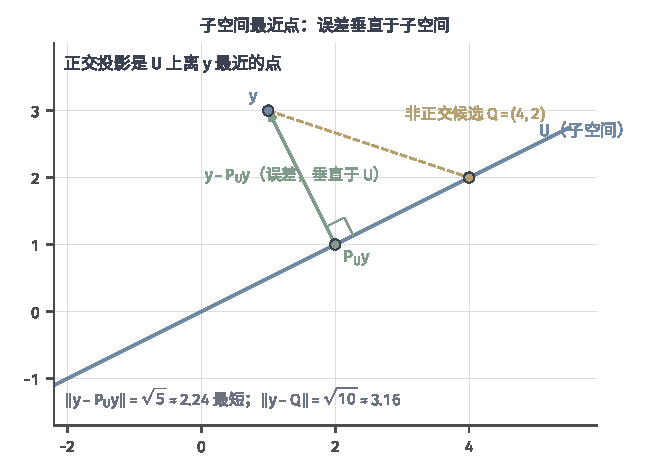
\includegraphics[width=112mm]{figures/01-mathematical-preliminaries-upper/02-linear-spaces/matplotlib/ls-orthogonal-projection-nearest/ls-orthogonal-projection-nearest.pdf}
  \caption{直线子空间$U$（过原点、方向$(2,1)$）上离$\bm y=(1,3)^\top$最近的点是正交投影
  $\bm p=(2,1)^\top$，误差$\bm y-\bm p=(-1,2)^\top$与$U$垂直（直角小方块）；
  同一线上的另一候选$\bm q=(4,2)^\top$到$\bm y$的距离$\sqrt{10}$明显大于最短距离$\sqrt5$。
  这是解析式教学构造。}
  \label{fig:ls-orthogonal-projection-nearest}
\end{figure}

\subsection{求解方法}

\subsubsection{正交化与QR分解}
\label{sec:ls-orthogonalization-qr}

一组向量$\bm q_1,\ldots,\bm q_r$若满足$\langle\bm q_i,\bm q_j\rangle=\delta_{i,j}$，即两两正交且长度为$1$，就称为标准正交组；它的Gram矩阵是单位阵，因而线性无关。张成$U$的标准正交组称为$U$的\term{标准正交基}（orthonormal basis）。
若$U$已有标准正交基$\bm q_1,\ldots,\bm q_r$，系数直接由内积读取：
$\bm p=\sum_j\bm q_j\langle\bm q_j,\bm y\rangle$，每个系数互不干扰。一般基没有这个
便利：基向量夹成斜坐标系，一个方向上的读数混入其他方向，逐个内积不能直接得到
独立系数。所以先把$\bm B$的列整理成正交列与上三角系数的乘积（QR分解），
再读取分量；这一步是把斜坐标换成直角坐标，而不改变点集$U$。

\paragraph{逐方向扣除与Gram--Schmidt}

\term{Gram--Schmidt正交化}按列进行。对$\bm b_j$，先减去它在已有正交方向上的分量：
\begin{equation}
 \bm v_j=\bm b_j-\sum_{i<j}\bm q_i\langle\bm q_i,\bm b_j\rangle,
 \qquad
 \bm q_j=\frac{\bm v_j}{\lVert\bm v_j\rVert_2}.
 \label{eq:ls-classical-gs}
\end{equation}
对$i<j$，$\langle\bm q_i,\bm v_j\rangle
=\langle\bm q_i,\bm b_j\rangle-\langle\bm q_i,\bm b_j\rangle=0$，
故每步$\bm v_j$与先前全部$\bm q_i$正交，归一化后得到新的标准正交方向；
归纳可知$\bm q_1,\ldots,\bm q_j$标准正交且与$\bm b_1,\ldots,\bm b_j$张成同一空间。
例如$\bm b_1=(1,0)^\top$直接给出$\bm q_1=(1,0)^\top$；
$\bm b_2=(1,1)^\top$扣除$\langle\bm q_1,\bm b_2\rangle\bm q_1=(1,0)^\top$后
得$\bm v_2=(0,1)^\top$，归一化即$\bm q_2=(0,1)^\top$。

\paragraph{正交列和上三角系数的形成}

把$\bm b_j=\sum_{i\leq j}r_{i,j}\bm q_i$中的系数$r_{i,j}=\langle\bm q_i,\bm b_j\rangle$
排成上三角矩阵$\bm R$，即得经济型\term{QR分解}
\begin{equation}
 \bm B=\bm Q\bm R,\qquad
 \bm Q^\top\bm Q=\bm I_r,\quad\bm R\text{ 上三角且对角元为正}.
 \label{eq:ls-qr-factorization}
\end{equation}
$\bm Q\in\mathbb R^{m\times r}$的列张成$U$，$\bm R$记录每列相对正交方向的组合系数。
图~\ref{fig:vol1-add-linear-qr-columns}给出最小的二维情形：保留第一条单位方向，
再从第二列减去它在第一方向上的分量，列空间不变，减去的部分记进$\bm R$。
\begin{figure}[!htb]
  \centering
  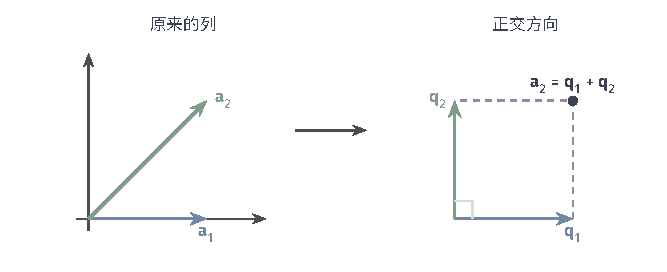
\includegraphics[width=112mm]{figures/01-mathematical-preliminaries-upper/02-linear-spaces/tikz/comprehension-additions/linear-qr-columns.pdf}
  \caption{QR把列的方向和组合系数分开。取$\bm a_1=(1,0)^\top$、$\bm a_2=(1,1)^\top$，
  正交化得到$\bm q_1=(1,0)^\top$、$\bm q_2=(0,1)^\top$，并有$\bm a_1=\bm q_1$、
  $\bm a_2=\bm q_1+\bm q_2$，故$\bm R=\left[\begin{smallmatrix}1&1\\0&1\end{smallmatrix}\right]$。
  虚线补出第二列的分量。}
  \label{fig:vol1-add-linear-qr-columns}
\end{figure}

若$\bm v_j=\bm0$，说明$\bm b_j$已由此前方向张成，输入列线性相关。
此时跳过该列、不执行归一化，或在$\bm R$中保留零系数位置；关键是不能用零向量作除数，
也不能把零长度当成正交失败而中断。归纳看$\bm v_j=\bm0$等价于
$\bm b_j\in\operatorname{span}\{\bm q_1,\ldots,\bm q_{j-1}\}$，空间没有扩大，
故跳过不影响后续列的投影。秩亏时仍得到$\bm B=\bm Q\bm R$，但$\bm R$奇异，
不能当作可逆三角矩阵回代；最近点$\bm p$作为$U$中的点仍唯一，但基系数不唯一，
需另选代表。例如$\bm b_1=(1,0)^\top$、$\bm b_2=(2,0)^\top$，
扣除后$\bm v_2=\bm b_2-2\bm q_1=\bm0$，跳过$\bm b_2$后$U$仍为$x$轴；
若强行归一化零向量会出现$0/0$。

\term{修正Gram--Schmidt}（modified Gram--Schmidt）
在每列扣除时，从当前残差出发依次向所有已有$\bm q_i$投影并立即更新残差，而不是
一次性减去全部旧分量：先$\bm v\leftarrow\bm b_j$，对$i=1,\ldots,j-1$逐次
$r_i=\bm q_i^\top\bm v$、$\bm v\leftarrow\bm v-r_i\bm q_i$，最后归一化。
精确算术中它与经典形式给出同一组正交方向；有限精度下，逐次更新残差使后续投影
基于已扣除的最新残差，正交性损失通常小于一次性扣除，差异由后续数值章节分析。

\paragraph{Householder反射的消元构造}

稠密计算常用\term{Householder反射}一次消去一列主对角线下的全部元素。
对非零实向量$\bm a$，取$s=1$当$a_1\geq0$否则$s=-1$，令
\begin{equation}
 \bm v=\bm a+s\lVert\bm a\rVert_2\bm e_1,\qquad
 \bm H=\bm I-2\frac{\bm v\bm v^\top}{\bm v^\top\bm v}.
 \label{eq:ls-householder}
\end{equation}
直接相乘可验$\bm H^\top\bm H=\bm I$（$\bm v$方向上反射两次回到原向量，
正交方向不变），且$\bm H\bm a=-s\lVert\bm a\rVert_2\bm e_1$：$\bm v$与
$\bm a+s\lVert\bm a\rVert_2\bm e_1$平行，反射把$\bm a$送到其关于该方向的镜像。
符号选择$s=\operatorname{sgn}(a_1)$避免在$\bm v$首元素中相减两个接近的数
（否则有效数字损失）。反射只作用于剩余子块，只需保存反射向量$\bm v$即可依次
应用$\bm H$，不必存整个$m\times m$正交矩阵。
例如$\bm a=(3,4)^\top$，$a_1>0$取$s=1$，$\lVert\bm a\rVert=5$，
$\bm v=(8,4)^\top$，$\bm v^\top\bm v=80$，
$\bm H=\bm I-2\bm v\bm v^\top/80$，计算得
$\bm H=\left[\begin{smallmatrix}-3/5&-4/5\\-4/5&3/5\end{smallmatrix}\right]$，
乘$\bm a$得$(-5,0)^\top$，确实把$\bm a$送到水平轴。

\paragraph{Givens旋转与局部消元}

\term{Givens旋转}在坐标$(i,j)$平面内作旋转，只消去一个指定元素：
\begin{equation}
 \bm G(i,j,\theta)=
 \begin{bmatrix}
  &\ddots&&\ddots\\
  &c&&s\\
  &&\ddots\\
  &-s&&c\\
  &&&\ddots
 \end{bmatrix},
 \qquad c^2+s^2=1,
 \label{eq:ls-givens}
\end{equation}
它只混合第$i,j$两个坐标，其余分量不变。选择$c,s$使第$j$坐标被旋到第$i$坐标、
目标位置归零：对$(a_i,a_j)$取$r=\sqrt{a_i^2+a_j^2}$，
$c=a_i/r$、$s=a_j/r$。新的一对分量为
$(c a_i+s a_j,\,-s a_i+c a_j)$，第二式$-s a_i+c a_j=0$，
第一式$c a_i+s a_j=r$。以$(a_i,a_j)=(3,4)$为例，$r=5$，
$c=3/5$、$s=4/5$，第一分量$c a_i+s a_j=9/5+16/5=5$，
第二分量$-s a_i+c a_j=-12/5+12/5=0$，变换后该对变为$(5,0)$，
非零元素只留在第$i$位置。$r=0$时两坐标已为零，
直接跳过、不必构造旋转。它改动范围小，适合稀疏、带状矩阵和逐列增量更新，
也是后文小型最小二乘问题逐步QR更新的工具；与Householder一次消去整列相比，
Givens每次只消一个元素，运算量更大但只触碰局部非零结构，稀疏优势明显。
图~\ref{fig:ls-givens-householder-elimination}把两种初等正交变换并置：
左图Givens旋转沿圆弧把$(a,b)=(2,1)^\top$旋到$(r,0)^\top$，右图Householder反射
沿角平分线把它映到同一位置，二者都保持长度而只改方向。

\begin{figure*}[htbp]
  \centering
  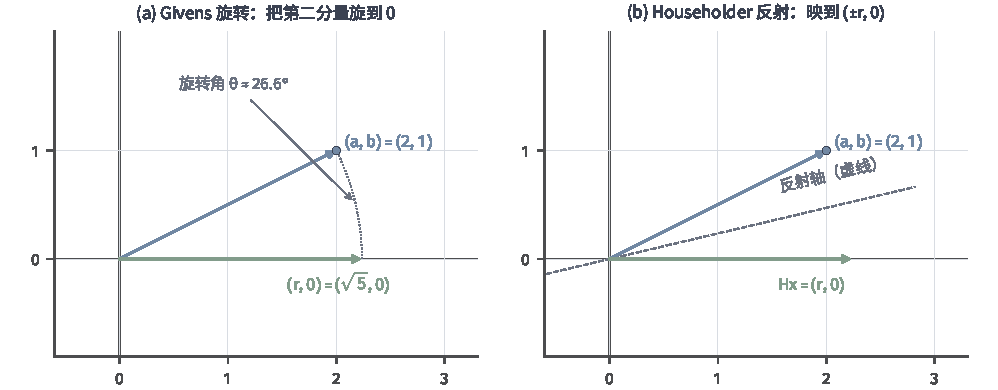
\includegraphics[width=168.998mm]{figures/01-mathematical-preliminaries-upper/02-linear-spaces/matplotlib/ls-givens-householder-elimination/ls-givens-householder-elimination.pdf}
  \caption{两种初等正交消元。左：Givens旋转把$(a,b)=(2,1)^\top$沿圆弧旋到
  $(r,0)^\top$，$r=\sqrt5$，旋转角$\theta=\arctan(1/2)$；右：Householder反射沿角平分线
  把同一向量映到$(r,0)^\top$。两者都是正交变换，保持长度，区别在旋转（行列式$+1$）与
  反射（对称正交）。解析式教学构造。}
  \label{fig:ls-givens-householder-elimination}
\end{figure*}

稠密$m\times d$矩阵的QR约需$2md^2-2d^3/3$次基本浮点运算，
正交列可由反射向量隐式保存，多个右端可以复用全部反射与$\bm R$，
新增一列只需对已有$\bm Q$追加一次投影与正交化，不必整体重做。
稀疏情形按非零结构只触碰局部元素，Givens适合这种逐元素增量更新。
秩亏时QR表示仍然成立，但回代与秩判断需要列置换（选最大模列提前作主元）等补充手段，
判定小$\lvert r_{j,j}\rvert$是数值精度问题而非精确代数结论，阈值与扰动由后续章节
说明。经济型QR只保留$r$列$\bm Q$，节省$m-r$列存储。

\subsubsection{最近点计算}

把候选点写成$\bm p=\bm B\bm c$。存在性一节的反向判据把
“最小距离”换成可直接检验的正交条件：最近点的残差$\bm r=\bm y-\bm B\bm c$必须与
每个基向量$\bm b_i$正交。这个条件不要求预先知道最小值，也不要求对$\bm c$逐点
比较距离，只要求列出$\dim U$个正交方程，把连续最小化变成线性系统求解；它是
可直接核验的一阶条件，满足时由勾股恒等式自动保证全局最小。几何上，残差垂直落
到$U$上，垂足即最近点。

\paragraph{正交残差条件与Gram系统}

标准内积下条件为$\bm B^\top(\bm y-\bm B\bm c)=\bm0$，即
\begin{equation}
 \bm G\bm c=\bm B^\top\bm y,\qquad
 g_{i,j}=\langle\bm b_i,\bm b_j\rangle.
 \label{eq:ls-gram-system}
\end{equation}
逐行写就是$\sum_j\langle\bm b_i,\bm b_j\rangle c_j=\langle\bm b_i,\bm y\rangle$，
即残差与每个基向量正交的$\dim U$个方程。加权内积下改为
$\bm B^\top\bm M(\bm y-\bm B\bm c)=\bm0$，Gram矩阵换成$\bm B^\top\bm M\bm B$。
\ref{sec:ls-orthogonality}已说明：基向量线性无关时，对任意非零$\bm c$有
$\bm c^\top\bm G\bm c=\lVert\bm B\bm c\rVert_2^2>0$，故$\bm G$正定、系统可逆。
边界：若基相关，$\bm G$奇异，方程仍相容但系数不唯一，最近点作为点仍唯一。

$\bm G$正定时方程~\eqref{eq:ls-gram-system}有唯一解$\bm c$，
对应唯一最近点$\bm p=\bm B\bm c$；权重$\bm M$正定时加权Gram矩阵
$\bm B^\top\bm M\bm B$同样正定（对非零$\bm c$有
$\bm c^\top\bm B^\top\bm M\bm B\bm c=\lVert\bm B\bm c\rVert_{\bm M}^2>0$），
同一结论保持。基相关时$\bm G$奇异、系数不唯一（同一$\bm p$
有多种组合），但最近点$\bm p$作为$U$中的点仍唯一，只需要再按准则选系数代表；
例如$\bm b_2=2\bm b_1$时，$\bm p=\bm b_1$可写成$\bm c=(1,0)$或$(0,1/2)$，
点相同而系数不同。

由$\bm B=\bm Q\bm R$，$\bm R$可逆时$\bm p=\bm Q\bm Q^\top\bm y$：
先算$\bm Q^\top\bm y$，再解三角系统$\bm R\bm c=\bm Q^\top\bm y$恢复系数，
最后$\bm p=\bm B\bm c$。由于$\bm Q^\top\bm Q=\bm I$，
$\bm Q^\top\bm y$的分量就是各正交方向上的坐标，无需先解Gram系统。
这条路线不显式形成Gram矩阵；形成正规乘积造成的尺度损失由后续章节用条件数解释。

核验分三步：$\bm p=\bm B\bm c\in U$；残差$\bm r=\bm y-\bm p$与$\bm B$各列正交；
报告最小距离$\lVert\bm r\rVert_2$。加权内积改变最近点，例~\ref{ex:linear-algebra-weighted-projection}
在同一直线上比较两种度量。
\begin{example}[同一子空间的两种最近点]
\label{ex:linear-algebra-weighted-projection}
在$\mathbb R^2$中取目标$\bm y=(2,1)^\top$、$U=\operatorname{span}\{(1,1)^\top\}$，
最近点写成$a(1,1)^\top$。欧氏投影最小化$(2-a)^2+(1-a)^2$，
导数给出$2a=3$，故$\bm p=(1.5,1.5)^\top$。
改用$\bm M=\operatorname{diag}(1,4)$，目标函数为$(2-a)^2+4(1-a)^2$，
导数给出$10a=12$，即$5a=6$，得到$\bm p_{\bm M}=(1.2,1.2)^\top$。
第二坐标误差代价更大，最近点便向$b_2=1$靠近；
残差$(0.8,-0.2)^\top$与$(1,1)^\top$的普通内积为$0.6\neq0$，
加权内积$0.8\cdot1+4(-0.2)\cdot1=0$，正交性必须用所选内积判断。
\end{example}
\begin{figure*}[htbp]
  \centering
  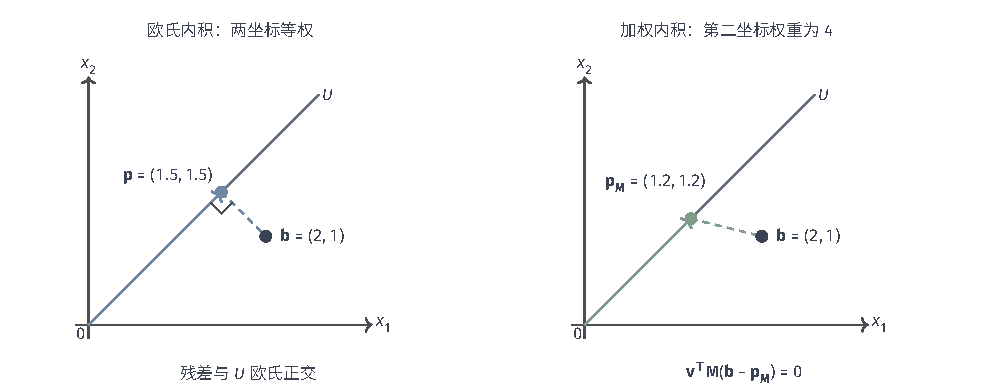
\includegraphics[width=168.998mm]{figures/01-mathematical-preliminaries-upper/02-linear-spaces/tikz/linear-algebra-weighted-projection/figure.pdf}
  \caption{同一目标在同一直线上的欧氏投影与加权投影。实箭头是投影向量，虚线是残差；
  右图画在普通坐标中，残差不必形成欧氏直角。正交性必须用所选内积判断。}
  \label{fig:linear-algebra-weighted-projection}
\end{figure*}

\subsection{投影的性质}

\paragraph{正交投影、斜投影与幂等}

标准内积下，以$\bm Q$为标准正交基的正交投影为
\begin{equation}
 \bm P_U=\bm Q\bm Q^\top,\qquad
 \bm P_U^\top=\bm P_U,\qquad \bm P_U^2=\bm P_U.
 \label{eq:linear-algebra-orthogonal-projector}
\end{equation}
它同时满足三条可逐条核验的性质：
\begin{enumerate}
 \item \term{幂等}（idempotent）：$\bm P_U^2=\bm Q\bm Q^\top\bm Q\bm Q^\top=\bm Q\bm Q^\top$，
 作用两次等于作用一次。
 \item 自伴（标准内积下$\bm P_U^\top=\bm P_U$）：保证残差与像正交，即欧氏最近点。
 \item 像为$U$：$\operatorname{range}\bm P_U=\operatorname{range}\bm Q=U$。
\end{enumerate}
但一般幂等映射只是沿某个方向把空间投到像上，
残差不必与像正交，也未必是最近点，这种映射称为\term{斜投影}（oblique projection）；
只有自伴的幂等映射才是正交投影。
例如$\bm P=\left[\begin{smallmatrix}1&-1\\0&0\end{smallmatrix}\right]$满足
$\bm P^2=\bm P$，把$(x,y)^\top$投到$x$轴上的$(x-y,0)^\top$，但
$\bm P^\top\neq\bm P$，残差$(y,y)^\top$不与$x$轴正交（普通内积$y\cdot0+y\cdot1=y\neq0$），
因而不是欧氏最近点。判别顺序：先验幂等（是否投影），再验对称（是否正交），
不能见幂等就当作最近点映射。

两个正交投影的复合一般不可交换：$\bm P_U\bm P_V\neq\bm P_V\bm P_U$，
乘积也未必仍是投影（两次投影的像一般既不是$U$也不是$V$）。两者可交换时，乘积
幂等且自伴，其像为$U\cap V$。反复投影怎样收敛到交空间属于序列极限问题，
留给后续收敛章节分析，这里不声称一次复合给出极限。

\section{线性方程：精确求解}
\label{sec:ls-exact-linear-equations}
\label{sec:linear-algebra-exact-systems}

\subsection{方程与条件}

给定$\bm A\in\mathbb R^{m\times d}$与目标$\bm b\in\mathbb R^m$，精确方程为
\begin{equation}
 \bm A\bm x=\bm b,\qquad \bm x\in\mathbb R^d.
 \label{eq:linear-algebra-linear-system}
\end{equation}
多个右端写成$\bm A\bm X=\bm B$，$\bm X\in\mathbb R^{d\times s}$、$\bm B\in\mathbb R^{m\times s}$；
它逐列等价于$s$个同系数矩阵的单右端方程$\bm A\bm x_j=\bm b_j$。
同一个$\bm A$的分解或迭代设置可按列复用，但每一列的相容性与残差要分别核验，
不能用一列的残差代替另一列。

按形状分：$m=d$为方阵，$m>d$为超定（方程多于未知量），$m<d$为欠定。
形状只限制秩的上限，不能单独判断有没有解：例如$\bm A=\left[\begin{smallmatrix}1\\1\end{smallmatrix}\right]$
是超定系统，但$\bm b=(1,1)^\top$在列空间内，因而相容且唯一；
而两行相同的方阵$\bm A=\left[\begin{smallmatrix}1&1\\1&1\end{smallmatrix}\right]$配
$\bm b=(1,2)^\top$就不相容。是否存在解由右端与值域的关系决定，
是否唯一由零空间决定，下面先判这两件事。

本节要求等式严格成立；浮点计算中“精确”表现为残差小到
给定容限，容限取值、舍入积累与条件数由后续章节处理。这里先在代数层面区分无解、
唯一解与多解，不能由某个算法算不出解就推断问题无解——算法失败可能只是数值或
实现问题，与代数相容性是两回事。

\subsection{存在性、唯一性与选解}

\subsubsection{相容性}
\label{sec:ls-compatibility}

$\bm A\bm x$是$\bm A$各列以$\bm x$为系数的线性组合，因此
$\bm A\bm x=\bm b$有解当且仅当$\bm b\in\operatorname{range}(\bm A)
=\operatorname{span}\{\bm a_1,\ldots,\bm a_d\}$。这一条件称为\term{相容}
（consistent）；不相容时任何输入都不能精确产生$\bm b$。判据直接来自列空间定义：
可达输出恰好是列的全部线性组合。例如$\bm A=\left[\begin{smallmatrix}1&1\\0&1\end{smallmatrix}\right]$，
两列$(1,0)^\top,(1,1)^\top$线性无关，列空间是全$\mathbb R^2$，任意右端都可达；
若把第二列换成$(1,1)^\top$使两列相同，列空间只是一条直线，垂直于它的右端就
不可达。形状（方程数多少）不决定可达性，列张成的空间才决定。

标准内积下有四个基本子空间：值域$\operatorname{range}(\bm A)$
与零空间$\operatorname{null}(\bm A)=\{\bm x:\bm A\bm x=\bm0\}$，
行空间$\operatorname{range}(\bm A^\top)$与左零空间
$\operatorname{null}(\bm A^\top)=\{\bm y:\bm A^\top\bm y=\bm0\}$。
由\ref{sec:ls-adjoints}建立的伴随恒等式
$\langle\bm y,\bm A\bm x\rangle=\langle\bm A^\top\bm y,\bm x\rangle$
是下面正交互补关系的依据：它把输出空间的配对转成输入空间的配对，使两个正交
关系不必另行假设。四个子空间分属输入、输出两个空间，不要混在同一侧。

若$\bm y\in\operatorname{null}(\bm A^\top)$，则对任意$\bm x$有
$\bm y^\top(\bm A\bm x)=(\bm A^\top\bm y)^\top\bm x=0$，故
$\operatorname{null}(\bm A^\top)\subseteq\operatorname{range}(\bm A)^\perp$；
维数互补给出反向包含，于是
\begin{equation}
 \operatorname{range}(\bm A)^\perp=\operatorname{null}(\bm A^\top).
 \label{eq:ls-range-leftnull-orthogonal}
\end{equation}

同理，$\operatorname{range}(\bm A^\top)^\perp
=\operatorname{null}(\bm A)$：若$\bm x\in\operatorname{null}(\bm A)$，则对任意
$\bm A^\top\bm y$有$(\bm A^\top\bm y)^\top\bm x=\bm y^\top\bm A\bm x=0$，
反向包含由维数互补得到。输入空间因此正交直和分解为
$\operatorname{null}(\bm A)\oplus\operatorname{range}(\bm A^\top)$，
输出空间分解为$\operatorname{range}(\bm A)\oplus\operatorname{null}(\bm A^\top)$。
前者记录被映射消去的输入方向，后者记录达不到的输出方向。

$\bm A\bm x=\bm b$相容的几何判据是$\bm b\in\operatorname{range}(\bm A)$，
即$\bm b$落在列空间内。等价地，由式~\eqref{eq:ls-range-leftnull-orthogonal}，
$\bm b$与左零空间正交：$\bm y^\top\bm b=0$对一切$\bm y\in\operatorname{null}(\bm A^\top)$
成立。前面的最近点结果将用于：不相容时求离$\bm b$最近的可达输出，
这是后续最小二乘任务的入口；本节只在相容前提下求精确解，不做残差最小化，
也不把“最近点”冒充为“解”。判据对任意形状的$\bm A$都适用，与$m,d$谁大无关。

\paragraph{增广矩阵的秩判据}

把$\bm b$并入系数矩阵得到增广矩阵$[\bm A\;\bm b]$。
$\bm b$是列的组合，当且仅当并入它不增加列空间维数，即
\begin{equation}
 \operatorname{rank}[\bm A\;\bm b]=\operatorname{rank}(\bm A).
 \label{eq:ls-augmented-rank}
\end{equation}
这是消元可直接检验的代数判据；不等号出现即无解。理由：若$\bm b$已在列空间内，
并入不扩大张成空间，秩不变；否则秩增加一。例如
$\bm A=\left[\begin{smallmatrix}1&1\\1&1\end{smallmatrix}\right]$的秩为$1$，
$\bm b=(1,2)^\top$使$[\bm A\;\bm b]$秩为$2$，判据直接给出无解；
而$\bm b=(1,1)^\top$并入后秩仍为$1$，相容。

不相容可由左零空间直接证明：若存在
$\bm y\in\operatorname{null}(\bm A^\top)$使$\bm y^\top\bm b\neq0$，
则所有可达输出$\bm A\bm x$在$\bm y$方向读数为
$\bm y^\top\bm A\bm x=(\bm A^\top\bm y)^\top\bm x=0$，而$\bm b$非零，
故$\bm b$不可达。上例中$\bm y=(1,-1)^\top$满足
$\bm A^\top\bm y=0$，而$\bm y^\top\bm b=1-2=-1\neq0$，这就是不可达证书。
反之，$\bm y^\top\bm b=0$对全部$\bm y\in\operatorname{null}(\bm A^\top)$
成立时，由式~\eqref{eq:ls-range-leftnull-orthogonal}知$\bm b$与左零空间正交，
即$\bm b\in\operatorname{range}(\bm A)$。证书法与秩判据等价，但给出一个可
直接核验的向量。

$\bm A\bm X=\bm B$相容当且仅当每一列
$\bm b_j\in\operatorname{range}(\bm A)$，等价于
$\operatorname{rank}[\bm A\;\bm B]=\operatorname{rank}(\bm A)$，
也等价于所有$\bm y\in\operatorname{null}(\bm A^\top)$满足$\bm y^\top\bm B=\bm0$。
各列独立判断，不能用一列相容代替另一列；逐列残差分别核验。

\subsubsection{唯一性与自由度}
\label{sec:ls-uniqueness-freedom}

设$\bm x_1,\bm x_2$都是解，则
$\bm A(\bm x_1-\bm x_2)=\bm b-\bm b=\bm0$，两解之差属于零空间
$\operatorname{null}(\bm A)$；反之，若$\bm x_0$是解且
$\bm n\in\operatorname{null}(\bm A)$，则$\bm A(\bm x_0+\bm n)=\bm b+\bm0=\bm b$，
故$\bm x_0+\bm n$也是解。这一双向关系说明：解集合恰好是“一个特解平移零空间”，
没有其他点混入。

\paragraph{特解加零空间的全部解}

相容时任取一个特解$\bm x_0$，全部解恰为
\begin{equation}
 \bm x=\bm x_0+\operatorname{null}(\bm A).
 \label{eq:ls-affine-solution-set}
\end{equation}
这是一个平移后的线性子空间，即\term{仿射空间}（affine space）：基点$\bm x_0$
不唯一，更换基点只平移集合，方向空间$\operatorname{null}(\bm A)$由全部点差唯一确定。
商空间把这种不可区分性表达为精确对应：
$\mathbb R^d/\operatorname{null}(\bm A)\to\operatorname{range}(\bm A)$，
$\bm x+\operatorname{null}(\bm A)\mapsto\bm A\bm x$良定义、线性、单射且满射，
却尚未在每个类中选代表。例如$x_1+x_2=2$有特解$(1,1)^\top$，零空间由
$(1,-1)^\top$张成，全部解为$(1,1)^\top+t(1,-1)^\top$，$t$任意；
$(1,0)^\top$与$(0,1)^\top$在$\bm A=(1,1)$下同属一类、只记录系数和。
\label{sec:linear-algebra-affine-relations}
图~\ref{fig:vol1-add-linear-nullspace-fibers}以$\bm A=(1,1)$展示：每条平行线
$x_1+x_2=c$对应同一个输出数，整条线归为一个原像类。
\begin{figure}[!htb]
  \centering
  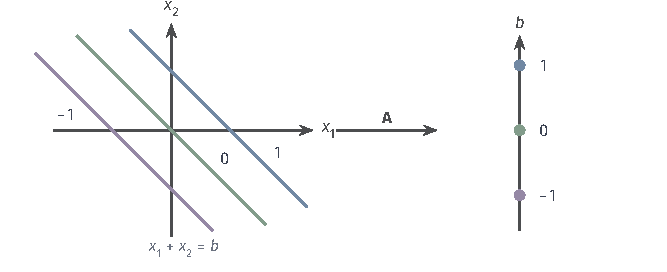
\includegraphics[width=112mm]{figures/01-mathematical-preliminaries-upper/02-linear-spaces/tikz/comprehension-additions/linear-nullspace-fibers.pdf}
  \caption{同一输出对应的整组输入。对$\bm A=(1,1)$，蓝、绿、紫直线分别满足
  $x_1+x_2=1,0,-1$；右侧同色点是各直线的输出。绿色直线是$\ker\bm A$，
  其余直线是它的平移。把一整条直线归为一类后，才得到与可达输出的一一对应。}
  \label{fig:vol1-add-linear-nullspace-fibers}
\end{figure}

由秩零度定理~\ref{thm:ls-rank-nullity}，
$\dim\operatorname{null}(\bm A)=d-\operatorname{rank}(\bm A)$，
这就是自由参数的个数。相容时任一特解$\bm x_0$加上零空间的全部点构成解集，
解集是$d-r$维仿射空间，$r=\operatorname{rank}(\bm A)$；
每增加一个自由参数，就多一个沿零空间移动而不改变输出的方向，自由参数个数
与列数减秩一致。例如$\bm A=[1\ 1]$，$d=2,r=1$，自由参数$1$个，
解$\bm x=(1,1)^\top+t(1,-1)^\top$中$t$即自由参数；$d-r=0$时零空间只含零向量，
自由参数为零，解唯一。

\paragraph{满列秩、满行秩与唯一性}

解唯一当且仅当$\operatorname{null}(\bm A)=\{\bm0\}$，
即满列秩$r=d$（$d$个列向量线性无关）：两解之差落在零空间，零空间为零向量迫使
两解相同。满行秩$r=m$只保证每个右端都可达（相容），
不保证唯一；满列秩保证唯一但不保证任意右端可达。两种满秩对应不同保证，
不能互换：满行秩可能欠定多解，满列秩可能超定不相容。例如$\bm A=(1,1)$满行秩
（$m=1$）但欠定，任意$\bm b$相容而解不唯一；$\bm A=(1,1)^\top$满列秩（$d=1$），
解唯一却只对$\bm b\in\operatorname{span}\{(1,1)^\top\}$相容。

超定$m>d$且满列秩时，相容则唯一解，不相容则无精确解（此时进入残差最小化任务）；
欠定$m<d$且满行秩时任意右端都相容，但至少有$d-m$个自由参数，解不唯一。
仅凭方程数与未知数个数不能下结论，必须回到实际秩与右端位置：超定也可能相容唯一，
方阵也可能无解。例如方阵$\bm A=\left[\begin{smallmatrix}1&1\\1&1\end{smallmatrix}\right]$
秩$1<d=2$，既多解又对$\bm b\notin\operatorname{span}\{(1,1)^\top\}$无解，
形状为方阵却不具备可逆性。

$\bm A=\bm0$时：$\bm b=\bm0$则任意$\bm x$都是解
（零空间为全空间$\mathbb R^d$，列空间为$\{0\}$），$\bm b\neq\bm0$则无解
（零右端落在列空间$\{0\}$内，非零右端不在）。反过来$\bm b=\bm0$而$\bm A\neq0$
时齐次方程$\bm A\bm x=\bm0$恒相容，至少有零解，秩亏时另有非零解。
这种边界不能套用含零分母的求逆公式（$\bm A^{-1}$不存在），直接按上述秩与值域
判据判断，避免对零矩阵作除法。

\subsubsection{多解中的选择}
\label{sec:ls-select-among-solutions}

相容而秩亏时，全部解是$\bm x_0+\operatorname{null}(\bm A)$，
等式本身不再挑选代表，需要额外准则。常用的是在解集中取欧氏范数最小者；
更换输入内积，代表点一般随之改变，准则必须先声明，不能默认“解”唯一。
这一准则与6.1的最近点几何一致：在平移仿射集合上找离原点最近的点，
垂足落在零空间的正交补上。

把任意解按输入空间的正交直和分解为
$\bm x=\bm x_\perp+\bm x_N$，其中$\bm x_N\in\operatorname{null}(\bm A)$，
$\bm x_\perp\in\operatorname{null}(\bm A)^\perp=\operatorname{range}(\bm A^\top)$。
$\bm A\bm x_N=\bm0$，输出只由$\bm x_\perp$决定，核分量对输出毫无贡献；
两个分量正交，故可分开处理。

\paragraph{最小范数精确解的唯一性}

两项正交，故
$\lVert\bm x\rVert_2^2=\lVert\bm x_\perp\rVert_2^2+\lVert\bm x_N\rVert_2^2$。
保持$\bm x_\perp$不变而去掉$\bm x_N$，输出不变（$\bm A\bm x_N=0$）且范数
严格减小；唯一最小范数代表就是$\bm x_N=0$的那个解，它落在
$\operatorname{null}(\bm A)^\perp$中。上例$x_1+x_2=2$的解
$(1+t,1-t)^\top$中，范数平方为$(1+t)^2+(1-t)^2=2+2t^2$，令核分量$t=0$
得$(1,1)^\top$，其范数$\sqrt2$小于$t\neq0$时的$\sqrt{2+2t^2}$。
映射$\bm A|_{\operatorname{null}(\bm A)^\perp}:
\operatorname{null}(\bm A)^\perp\to\operatorname{range}(\bm A)$是双射：
单射来自交为零，满射来自上述分解，故最小范数代表存在且唯一。

满列秩时$\bm A^\top\bm A$正定，存在左逆
$\bm L=(\bm A^\top\bm A)^{-1}\bm A^\top$使$\bm L\bm A=\bm I$，
它能恢复全部输入，但只对值域中的输出反演；满行秩时存在右逆
$\bm R=\bm A^\top(\bm A\bm A^\top)^{-1}$使$\bm A\bm R=\bm I$，
它为每个输出挑一个输入，却不能恢复被零空间消去的信息。单侧逆一般不唯一：
例如$\bm A=(1,0)^\top$，任意$\bm L=(1,t)$都满足$\bm L\bm A=1$，
$t$任意而不破坏左逆。它们是代数公式，实际通过三角求解应用，不显式形成逆矩阵；
左逆对应唯一解（满列秩），右逆对应一种选解（满行秩）。

最小范数代表依赖指定的输入内积；一般权重或正则化会同时改变目标与代表，
完整的伪逆构造、任意秩处理与加权选解放在后续残差最小一节。本节只确认：多解时等式不唯一，
必须先声明准则再谈“解”；在未声明准则前，报告“一个解”而非“那个解”。
满行秩右逆给出的代表只是众多选解之一，未必是最小范数代表，二者不可混称。

\subsection{直接法}
\label{sec:ls-direct-methods}
\label{sec:linear-algebra-direct-exact}
\label{sec:matrix-analysis-stable-solvers}

直接法在有限步内把方程化为可逐个求解的三角或块系统。它需要显式读取并存储因子，
适用于矩阵可整体获得、规模可控或多右端复用同一因子的情形。

\subsubsection{消元与LU分解}

高斯消元用一行的倍数消去另一行的某个系数，
行变换（把某行加到另一行、交换两行、某行乘非零常数）不改变解集。例如
$\left[\begin{smallmatrix}2&1\\4&3\end{smallmatrix}\right]\bm x=(1,3)^\top$，
第二行减去第一行的两倍得$(0,1)$对应$x_2=1$，再代回$2x_1+1=1$得$x_1=0$。
多步消元记录下来就是三角因子，不必每次从头回代。

第$k$步在尚未处理的第$k$列中选择绝对值最大的可用元素移到主元位置，
再消去它下方的元素；记录的行交换累计为置换矩阵$\bm P$。例如主元位置为零而其下方
同列有非零元时，交换两行即可继续；部分主元避免把本可交换避开的零元素拿来作除数，
也抑制乘子$l_{i,k}=a_{i,k}/a_{k,k}$过大带来的放大。但交换不会把奇异矩阵变成
可逆矩阵：秩由列张成决定，行置换只重排方程，不改变秩与相容性。

\paragraph{消元乘子与LU因子}

消去乘子$l_{i,k}=a^{(k)}_{i,k}/a^{(k)}_{k,k}$进入单位下三角
因子$\bm L$，剩余系数构成上三角因子$\bm U$，得到带部分主元的分解
\begin{equation}
 \bm P\bm A=\bm L\bm U,
 \label{eq:matrix-analysis-palu}
\end{equation}
其中$\bm L$单位下三角（对角为1）、$\bm U$上三角。乘子就是第$k$步消去第$i$行
第$k$列所用的倍数，被原样留在$\bm L$中，使$\bm L\bm U$乘回可复原置换后的
系数矩阵；前面列的乘子随行交换同步更新。验证方式：把$\bm L\bm U$逐项乘回，
与$\bm P\bm A$比较，不必另行求解。

消元得到的阶梯形直接显示秩：每选到一个非零主元秩加一；精确算术中某列无可用主元，
说明矩阵秩亏，此时应转入秩判断并按6.2.1相容性判据核验增广矩阵秩，而不是继续
除以零。对相容的秩亏系统，自由变量取零即得一个特解，其余解沿零空间展开；
对不相容系统，阶梯形会出现$0=\text{非零}$的矛盾行，直接判定无解。
某个小主元不能独自证明精确奇异，浮点阈值决定的数值秩留待后续章节说明；
代数上的奇异（主元恰为零）与数值上的接近奇异（主元很小但非零）是两件事。

分解后依次解$\bm L\bm z=\bm P\bm b$（前代，从前向后）与
$\bm U\bm x=\bm z$（回代，从后向前）：
\begin{equation}
 z_i=(\bm P\bm b)_i-\sum_{j<i}l_{i,j}z_j,\qquad
 x_i=\frac{z_i-\sum_{j>i}u_{i,j}x_j}{u_{i,i}}.
\end{equation}
回到开头的例子，消元后$\bm U=\left[\begin{smallmatrix}2&1\\0&1\end{smallmatrix}\right]$、
$\bm L=\left[\begin{smallmatrix}1&0\\2&1\end{smallmatrix}\right]$，
先由$\bm L\bm z=(1,3)^\top$得$z_1=1$、$z_2=1$，再回代$x_2=1$、
$2x_1+1=1$得$x_1=0$。解出后代回原方程核验$\bm A\bm x=\bm b$。

因子$\bm L,\bm U$（或置换$\bm P$）只建立一次，每个新右端$\bm b_j$各自完成两次
三角求解$\bm L\bm z_j=\bm P\bm b_j$、$\bm U\bm x_j=\bm z_j$，不必为每列重做
$O(d^3)$分解；当同一$\bm A$搭配多列$\bm B$时，分摊成本主要落在$O(d^2)$的逐列
三角求解上。矩阵改变后不能无条件复用旧因子：结构或元素变化使$\bm L\bm U$不再等于
新的$\bm P\bm A$，须重新分解；仅有右端变化才允许复用。

稠密$d\times d$矩阵的LU分解约需$2d^3/3$次基本浮点运算，
每个新右端的两次三角求解为$O(d^2)$，存储$O(d^2)$。稀疏矩阵消元可能产生原来
没有的非零元，称为\term{填充}（fill-in），使原本稀疏的因子退化为准稠密；
存储收益还取决于行列排序与结构，而不只看原始非零元数。因此稀疏直接法的成本
不能只用原始非零元数估计。

\subsubsection{Cholesky分解}

当$\bm A=\bm A^\top\succ0$（对称正定）时，
定理~\ref{thm:ls-gram-factor}的配方原理已说明正定矩阵可归纳写成$\bm L\bm L^\top$
形式；本节把它落实为可逐列执行的三角求解算法。Cholesky 能省去 LU 的选主元，前提可拆成
三条同时成立：
\begin{enumerate}
 \item 对称性$\bm A=\bm A^\top$：只需存储一个三角因子，配方只作用于上半。
 \item 正定性$\bm x^\top\bm A\bm x>0$（$\bm x\neq\bm0$）：等价于各阶顺序主子式为正，
 配方剩余$a_{j,j}-\sum_{k<j}l_{j,k}^2>0$恒成立。
 \item 由此每步主元严格为正：无需行交换，不会出现零主元或负数开方。
\end{enumerate}
这是它相对LU的简化前提。

把第一个坐标与其余坐标分块配方，消去首变量后剩余的系数矩阵
仍正定，因而每一步的主元严格为正；按维数归纳即可逐列构造因子。具体地，正定二次型
对首变量配成完全平方，平方项系数为正，余下不含首变量的二次型由正定性仍正定，
这也解释了Cholesky每步剩余矩阵为何保持正定结构、根号内为何严格为正。这一归纳
正是定理~\ref{thm:ls-gram-factor}配方原理的逐步执行，不是另立假设。

\paragraph{Cholesky因子的逐列构造}

存在唯一对角元为正的下三角矩阵$\bm L$使
\begin{equation}
 \bm A=\bm L\bm L^\top,
 \label{eq:matrix-analysis-cholesky}
\end{equation}
称为\term{Cholesky分解}（Cholesky decomposition）。逐列计算
\begin{equation}
 l_{j,j}=\sqrt{a_{j,j}-\sum_{k<j}l_{j,k}^2},\qquad
 l_{i,j}=\frac{a_{i,j}-\sum_{k<j}l_{i,k}l_{j,k}}{l_{j,j}}\quad(i>j).
\end{equation}
第一式是第$j$个对角平方（配方剩余），第二式由$\bm L\bm L^\top$的$(i,j)$元
$a_{i,j}=\sum_{k\leq j}l_{i,k}l_{j,k}$反解得到。正定性保证根号内严格为正，
除法合法。例如$\bm A=\left[\begin{smallmatrix}4&2\\2&5\end{smallmatrix}\right]$，
先得$l_{11}=\sqrt4=2$，再$l_{21}=a_{21}/l_{11}=2/2=1$，最后
$l_{22}=\sqrt{5-l_{21}^2}=\sqrt{5-1}=2$，故
$\bm L=\left[\begin{smallmatrix}2&0\\1&2\end{smallmatrix}\right]$，
乘回$\bm L\bm L^\top=\left[\begin{smallmatrix}4&2\\2&5\end{smallmatrix}\right]$
逐项等于原矩阵。

每列由先前列唯一确定：式~\eqref{eq:matrix-analysis-cholesky}的$(i,j)$元给出
$a_{i,j}=\sum_{k\leq j}l_{i,k}l_{j,k}$，右侧$k<j$项已由先前因子确定，故$l_{i,j}$
被唯一反解；对角$l_{j,j}$由配方剩余开方，正对角约定又固定了开方符号（取$+$而非$-$），
因此带正对角的Cholesky分解唯一。若允许对角取负号，$\pm l_{j,j}$都满足乘积，符号未定，
正对角约定排除了这一任意性。对照LU：一般矩阵的LU在主元非零时也唯一，
而Cholesky额外靠正定性保证根号内为正、无需选主元。

求解依次用$\bm L\bm z=\bm b$（前代，$z_i=(b_i-\sum_{j<i}l_{i,j}z_j)/l_{i,i}$）与
$\bm L^\top\bm x=\bm z$（回代，$x_i=(z_i-\sum_{j>i}l_{j,i}x_j)/l_{i,i}$）。
稠密成本约$d^3/3$，只存一个三角因子（利用对称不复存上半），
约为LU的一半；多个右端复用同一因子，每个右端仍需两次三角求解$O(d^2)$。
复用前提仍是$\bm A$不变。

半正定时可能出现零主元（配方剩余为零），不能照搬上述除以$l_{j,j}$与开正根号的
步骤，否则$0/0$或负数开方。盲目加一个“小常数”会改变原方程、把退化系统改成另一
问题；应先区分真实退化（$\bm A$本有零空间、相容前提下进入选解）、约束造成的零空间
与数值误差（接近奇异而非精确奇异，阈值问题留后续章节）。只有任务本身明确引入阻尼
或惩罚时，才改用相应的正则化系统，不能为让算法通过而临时改动系数。

\subsubsection{LDL$^{\top}$分解}
\label{sec:ls-ldlt}

对称但不定（有正也有负方向）的矩阵不能逐项开正平方根：它既没有Cholesky所需的
正主元可开正根号，也没有CG所需的正分母，二者都不能沿用；例如$\operatorname{diag}(1,-1)$可逆却出现负主元，
$\sqrt{-1}$无实意义。对称结构仍然保留，可把符号和耦合
留在对角块中，这正是LDL$^{\top}$分解的用途：不开方、由$\bm D$的负块承接符号。

引入带对称置换的分解$\bm P\bm A\bm P^\top=\bm L\bm D\bm L^\top$，
其中$\bm L$单位下三角，$\bm D$由一阶与二阶对角块组成。
例如$\left[\begin{smallmatrix}0&1\\1&0\end{smallmatrix}\right]$可逆却没有可用的一阶对角主元；
同时交换行列以保留对称性，选择可逆的一阶或二阶块作主元，再消去与剩余变量的耦合。

\paragraph{LDL$^{\top}$因子的形成}

按块递归消去耦合。把当前待消矩阵分块为
$\begin{bmatrix}\bm A_{11}&\bm A_{12}\\\bm A_{21}&\bm A_{22}\end{bmatrix}$，
其中$\bm A_{11}$是选定的可逆一阶或二阶块；单位下三角乘子块取
$\bm L_{21}=\bm A_{21}\bm A_{11}^{-1}$，消去后剩余块为Schur补
$\bm A_{22}-\bm A_{21}\bm A_{11}^{-1}\bm A_{12}$，再对剩余块重复同一过程。
$\bm L$记录这些乘子（单位对角），$\bm D$保留各步选定的对角块（一阶标量或二阶
对称块）。不定矩阵的负主元不是算法失败，只是不能开平方；$\bm D$的负块直接
保留符号。每步乘回$\bm L\bm D\bm L^\top$逐项核对，确认乘积等于置换后的系数矩阵。
与Cholesky相比，LDL$^{\top}$不开根号、把符号集中在$\bm D$，因此可覆盖对称不定
与条件良好的半定情形；$\bm D$为一阶、二阶块正是为了在无正主元时仍取得可逆块。

一阶块$d$直接除以标量$d$：$y=z/d$。二阶块
$\begin{smallmatrix}d_{11}&d_{12}\\d_{12}&d_{22}\end{smallmatrix}$
解$\bm D\bm y=\bm z$，令$\Delta=d_{11}d_{22}-d_{12}^2$（非零由块主元可逆保证），
则
\begin{equation}
 y_1=\frac{d_{22}z_1-d_{12}z_2}{\Delta},\qquad
 y_2=\frac{d_{11}z_2-d_{12}z_1}{\Delta}.
\end{equation}
负对角元照常保留，不要求开平方；二阶块一次解完即可，不必再细分。例如二阶块
$\begin{smallmatrix}0&1\\1&0\end{smallmatrix}$（$d_{11}=0,d_{12}=1,d_{22}=0$）
行列式$\Delta=-1\neq0$，代入得$y_1=z_2$、$y_2=z_1$，直接解出两个未知量，
避免了寻找不存在的一阶零对角主元。

求解依次经过置换（把右端按$\bm P$重排）、下三角系统$\bm L\bm z=\bm P\bm b$
（前代）、小对角块系统$\bm D\bm y=\bm z$（逐块解一阶/二阶）和上三角系统
$\bm L^\top\bm x=\bm y$（回代），最后按置换$\bm P^\top$恢复原坐标；
每一步都是易解的三角或小块系统，回代次序与消元相反，置换把被交换的列/行位置
还原。这一链条与Cholesky两次三角求解平行，只是中间插入块对角求解与逆置换。

区分“具有负方向”（不定、$\bm D$出现负块）和“具有零空间”（奇异、$\bm D$出现
零块）：前者仍可唯一求解，负块只是符号；后者需重新判断相容性与选解，不能把零块
当可逆块作除法。这里只说明结构与求解路径，求解驻点方程不等于最小化对应的二次目标
（不定二次型无下界，驻点不是极小点）。

\subsubsection{QR分解}

前面建立的QR用正交变换把$\bm A$化为上三角。正交变换
保持欧氏长度，对相容方程$\bm A\bm x=\bm b$左乘$\bm Q^\top$后，方程拆成
可解的三角约束（前$d$行$\bm R\bm x=\bm Q^\top\bm b$）与自动满足的零残差行
（下方$\bm Q^\top\bm b$分量为零，这是相容条件$\bm b\in\operatorname{range}(\bm A)$
的投影表达），不需要额外极小化。不相容时下方残差非零，进入最小二乘任务而非本节。

$m\geq d$且满列秩时，经济型$\bm A=\bm Q\bm R$给出
$\bm R$可逆上三角；相容时解$\bm R\bm x=\bm Q^\top\bm b$，下方行的残差自动为零。
例如$\bm A=\left[\begin{smallmatrix}1&1\\1&0\\0&1\end{smallmatrix}\right]$，
两列线性无关；取相容右端$\bm b=(2,1,1)^\top=\bm A(1,1)^\top$。QR把$\bm A$
化为上三角，前两行$\bm R$可逆、第三行为零；左乘$\bm Q^\top$后第三行给出相容性核验
（此处$\bm Q^\top\bm b$第三分量为零），前两行的上三角系统回代得
$\bm x=(1,1)^\top$，代回$\bm A\bm x$得$(2,1,1)^\top=\bm b$。
若右端使第三分量非零，则方程不相容，转入后文最小二乘而非此处三角求解。

$m\leq d$且满行秩时对$\bm A^\top$作QR（即LQ分解，$\bm A=\bm L\bm Q^\top$），
在$\operatorname{range}(\bm A^\top)$内求解，使解落在零空间的正交补中，
自然得到最小范数方向上的代表。这与6.2.1“最小范数代表取在$\operatorname{null}(\bm A)^\perp$”
一致；转置QR只给满行秩情形一个选解路径，任意秩仍归SVD。

秩亏而相容时存在自由方向，解集为特解平移零空间；QR本身只给出一个满足方程的解，
不挑选最小范数代表。完整的任意秩选解工具（SVD，把解取在零空间正交补上）留待
后续残差最小章节，本节不声称普通QR已给出最小范数解。

列主元QR（QRCP）每步选模最大的未处理列提前作主元，重新安排列以辅助判断秩；
普通无主元QR的某个小对角元本身不是全部数值秩信息，可靠阈值还需要误差尺度
（条件数与扰动由后续章节给出）。无论用哪种QR，解出后仍须核验原方程残差
$\bm b-\bm A\bm x$，三角系统满足不等于原系统满足。

\subsubsection{分块消元与低秩更新}
\label{sec:matrix-analysis-blocks-updates}

先从最小的二元例子看消元在做什么。解
$\left[\begin{smallmatrix}2&1\\1&2\end{smallmatrix}\right](x_1,x_2)^\top=(1,3)^\top$：
第一式$2x_1+x_2=1$把$x_1=(1-x_2)/2$表示出来，代入第二式得
$(1-x_2)/2+2x_2=3$，乘$2$后$1+3x_2=6$，即$x_2=5/3$，回代$x_1=(1-5/3)/2=-1/3$。
核验：$2(-1/3)+5/3=1$、$(-1/3)+2(5/3)=3$。这里“用第一块消去第二块里的$x_1$”，
第二块剩下的系数$2-1\cdot(1/2)=3/2$，正是把$2\times2$矩阵左上元$2$作除后右下角的残留。
图~\ref{fig:ls-schur-block-elimination}把这一分块消元两步并置。

\begin{figure*}[htbp]
  \centering
  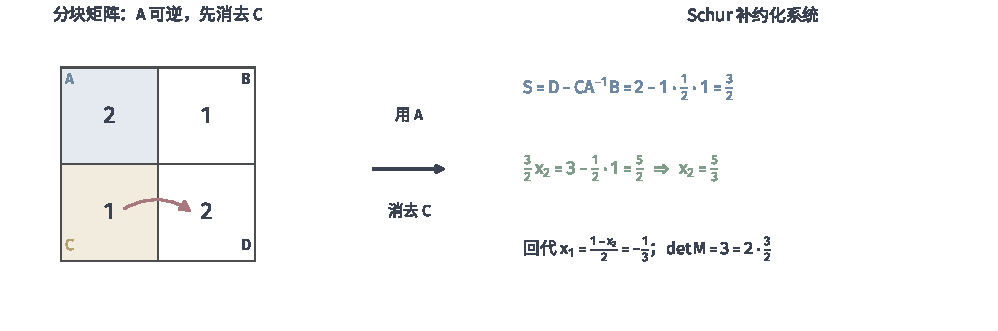
\includegraphics[width=168.998mm]{figures/01-mathematical-preliminaries-upper/02-linear-spaces/matplotlib/ls-schur-block-elimination/ls-schur-block-elimination.pdf}
  \caption{Schur 补的 2×2 分块消元。左：$\bm M=\left[\begin{smallmatrix}2&1\\1&2\end{smallmatrix}\right]$
  按左上块$\bm A=2$分块，先由第一行表出$x_1=(1-x_2)/2$；右：代入第二行后右下角残留
  Schur补$\bm S=3/2$，约化得$x_2=5/3$、回代$x_1=-1/3$，且$\det\bm M=2\cdot3/2=3$。
  解析式教学构造。}
  \label{fig:ls-schur-block-elimination}
\end{figure*}

下面把这一操作写成块记号。

把未知量分成两块，设
$\bm M=\left[\begin{smallmatrix}\bm A&\bm B\\\bm C&\bm D\end{smallmatrix}\right]$，
$\bm A\in\mathbb R^{p\times p}$可逆，右端$(\bm f^\top,\bm g^\top)^\top$。
第一组方程$\bm A\bm x+\bm B\bm y=\bm f$先把$\bm x=\bm A^{-1}(\bm f-\bm B\bm y)$
用$\bm y$表示，再代入第二组消去$\bm x$。典型来源是二部结构：全局参数块与各局部
块相连、局部块之间不直接相连，先分别消去各局部块，只剩全局块的小系统。

\paragraph{Schur补与约化系统}

\term{Schur补}（Schur complement）定义为
$\bm S=\bm D-\bm C\bm A^{-1}\bm B$。
\label{def:matrix-analysis-schur-complement}
代入第二组得到约化系统
\begin{equation}
 \bm S\bm y=\bm g-\bm C\bm A^{-1}\bm f,
 \label{eq:matrix-analysis-schur-complement}
\end{equation}
矩阵形式为
$\left[\begin{smallmatrix}\bm I&\bm0\\-\bm C\bm A^{-1}&\bm I\end{smallmatrix}\right]
\bm M=\left[\begin{smallmatrix}\bm A&\bm B\\\bm0&\bm S\end{smallmatrix}\right]$，
即左边乘一个单位下三角消去块左下角，把$\bm M$化成块上三角。在$\bm A$可逆
前提下，$\bm M$可逆当且仅当$\bm S$可逆，且$\det\bm M=\det\bm A\det\bm S$。
例如$\bm M=\left[\begin{smallmatrix}2&1\\1&2\end{smallmatrix}\right]$，
取$\bm A=2$、$\bm B=\bm C=1$、$\bm D=2$，则$\bm S=2-1/2=3/2$，
$\det\bm M=3=2\cdot3/2$，约化$3y/2=g-f/2$解出$y$后回代$x=(f-y)/2$。

解出$\bm y$后回代$\bm x=\bm A^{-1}(\bm f-\bm B\bm y)$。
逆通过求解$\bm A\bm Z=\bm B$、$\bm A\bm x=\bm f$来应用，不为套公式先形成整个
逆矩阵。需要时块逆为
\begin{equation}
 \bm M^{-1}=
 \begin{bmatrix}
  \bm A^{-1}+\bm A^{-1}\bm B\bm S^{-1}\bm C\bm A^{-1}
  &-\bm A^{-1}\bm B\bm S^{-1}\\
  -\bm S^{-1}\bm C\bm A^{-1}&\bm S^{-1}
 \end{bmatrix}.
 \label{eq:matrix-analysis-block-inverse}
\end{equation}
回代后必须代回原两块方程核验，约化系统相容不自动保证原方程每块满足。

$\bm M$对称时$\bm C=\bm B^\top$。配方给出
\begin{equation}
 \begin{bmatrix}\bm x\\\bm y\end{bmatrix}^{\top}
 \bm M\begin{bmatrix}\bm x\\\bm y\end{bmatrix}
 =(\bm x+\bm A^{-1}\bm B\bm y)^\top
 \bm A(\bm x+\bm A^{-1}\bm B\bm y)+\bm y^\top\bm S\bm y.
\end{equation}
右边两项分别为$\bm A$、$\bm S$的二次型。因此$\bm A\succ0$时
\begin{equation}
 \bm M\succ0\quad\Longleftrightarrow\quad
 \bm D-\bm B^\top\bm A^{-1}\bm B\succ0.
 \label{eq:matrix-analysis-schur-positive-definite}
\end{equation}
必要性可取$\bm x=-\bm A^{-1}\bm B\bm y$使第一项归零，只剩$\bm y^\top\bm S\bm y$
须对所有$\bm y$为正；充分性来自两项非负且不能同时为零（$\bm A$正定）。

对称正定等价于各阶顺序主子式为正，这正是逐块配方的主元；配方每步剩余矩阵正定，
故主元严格为正。半正定不能机械把严格不等号改为非严格，零主元对应真实退化，
主子式判据需另行处理零空间，不能套用正定除法；负主元（不定）则由LDL$^{\top}$
的块对角承接，不属Cholesky范围。

$\bm A$本身可能奇异，不能直接把$\bm A^{-1}$换成伪逆而不加条件；
需要$\operatorname{range}(\bm B)\subseteq\operatorname{range}(\bm A)$等值域条件
保证消去可行，以及伪逆版本的Schur补，再核验零空间是否留下自由参数。
不满足值域条件时，第一组方程$\bm A\bm x=\bm f-\bm B\bm y$对某些$\bm y$无解，
分块消元不能进行。

矩阵由$\bm A$变为$\bm A+\bm U\bm C\bm V^\top$，新增耦合只经过$k$个中间坐标
（$k$通常远小于$d$）。引入辅助未知量$\bm z=\bm V^\top\bm x$，把大系统换成$k$阶
小系统加已有$\bm A$的求解器，避免对$d$阶新矩阵重新分解；这是精确改变矩阵，不是
近似压缩，新矩阵与旧矩阵逐项不同。适用前提是旧求解器仍可用（$\bm A$可逆或已存
因子），$k$很小使小系统值得单独求解。

\paragraph{Woodbury恒等式与小系统}

设$\bm A$、$\bm C$与
$\bm S=\bm C^{-1}+\bm V^\top\bm A^{-1}\bm U$均可逆，按两种顺序消元同一块矩阵，
比较左上块得\term{Woodbury恒等式}
\begin{equation}
 (\bm A+\bm U\bm C\bm V^\top)^{-1}
 =\bm A^{-1}-\bm A^{-1}\bm U
 (\bm C^{-1}+\bm V^\top\bm A^{-1}\bm U)^{-1}
 \bm V^\top\bm A^{-1}.
 \label{eq:matrix-analysis-woodbury}
\end{equation}
取$\bm C=\bm I$时只需$\bm A$与$\bm I+\bm V^\top\bm A^{-1}\bm U$可逆，
无须对矩形$\bm U,\bm V$假定逆；实现为
$(\bm I+\bm V^\top\bm A^{-1}\bm U)\bm z=\bm V^\top\bm A^{-1}\bm b$，
再$\bm x=\bm A^{-1}(\bm b-\bm U\bm z)$。先消$\bm A$得小系统$\bm S$，
先消$\bm C^{-1}$得更新矩阵，两种消元左上块比较即得恒等式。

$k=1$时得Sherman--Morrison公式
$(\bm A+\bm u\bm v^\top)^{-1}
=\bm A^{-1}-\dfrac{\bm A^{-1}\bm u\bm v^\top\bm A^{-1}}
{1+\bm v^\top\bm A^{-1}\bm u}$，要求$1+\bm v^\top\bm A^{-1}\bm u\neq0$。
同一块行列式的两种消元给出
$\det(\bm A+\bm U\bm C\bm V^\top)
=\det\bm A\det\bm C\det\bm S$；行列式恒等式在小系统奇异时仍可能成立，
求逆公式则不能使用。例如$\bm A=\operatorname{diag}(2,3)$、
$\bm u=\bm v=(1,1)^\top$、$\bm b=(1,0)^\top$，直接解
$\left[\begin{smallmatrix}3&1\\1&4\end{smallmatrix}\right]\bm x=\bm b$
得$\bm x=(4/11,-1/11)^\top$，更新公式的标量
$1+\bm u^\top\bm A^{-1}\bm u=1+1/2+1/3=11/6$，代回同解，
行列式为$6\times11/6=11$。原分解已存在时，求$\bm A^{-1}\bm U$只需$k$次
三角求解；低秩更新精确改变矩阵，不是后文的低秩压缩任务，小系统接近奇异时公式
仍可能敏感。

\subsection{定常迭代法}
\label{sec:ls-stationary-iterations}
\label{sec:linear-algebra-stationary-splitting}

稀疏方程的一行往往只连接几个未知量，反复按行校正可以避免全局分解。
定常迭代每轮使用相同的校正规则；本节说明规则能否执行、怎样更新与核验，
收敛速率与暂态行为由后续收敛章节分析。

\subsubsection{矩阵分裂}

从近似解$\bm x^{(t)}$出发，定义当前残差
\begin{equation}
 \bm r^{(t)}=\bm b-\bm A\bm x^{(t)},
\end{equation}
它记录尚未消除的输出差距：$\bm r^{(t)}=\bm0$即精确解，否则方程要求再施加
$\bm A$把剩余差距补回。定常迭代不从零重建解，而只在当前近似上施加一轮校正，
因此每一步先有当前近似、才有要校正的残差。

把系数矩阵拆成$\bm A=\bm M-\bm N$，其中$\bm M$可逆且容易求解
（对角、三角、块对角或局部小系统），$\bm N$收集留给下一轮处理的耦合。
方程$\bm A\bm x=\bm b$改写为$\bm M\bm x=\bm N\bm x+\bm b$：把容易求解的
$\bm M$留在左端，难处理的耦合$\bm N\bm x$先用上一轮的值代入。这样每轮不必解
原系统，只解一个关于校正量的易解方程。分裂不是唯一的，同一$\bm A$可取不同
$\bm M$，直接决定每轮是否可执行、是否收敛；收敛性判据由后续收敛章节给出，
本节只保证方程可逐步更新。

\paragraph{残差校正的迭代公式}

定常迭代格式为
\begin{equation}
 \bm M\bm x^{(t+1)}=\bm N\bm x^{(t)}+\bm b,\qquad
 \bm x^{(t+1)}=\bm x^{(t)}+\bm M^{-1}\bm r^{(t)}.
 \label{eq:ls-stationary-splitting-form}
\end{equation}
第二式由$\bm M(\bm x^{(t+1)}-\bm x^{(t)})=\bm b-(\bm M-\bm N)\bm x^{(t)}
=\bm b-\bm A\bm x^{(t)}=\bm r^{(t)}$得到，校正量$\Delta\bm x=\bm M^{-1}\bm r^{(t)}$
正是“用易解的$\bm M$把当前残差反推成一次位移”。实现时只求
$\bm M\bm z=\bm r^{(t)}$再$\bm x^{(t+1)}=\bm x^{(t)}+\bm z$，不形成$\bm M^{-1}$；
形成逆矩阵既无必要，又会丢失$\bm M$容易求解的三角或对角结构。

设$\bm x_*$为精确解，由$\bm A\bm x_*=\bm b$与分裂$\bm A=\bm M-\bm N$，
误差$\bm e^{(t)}=\bm x^{(t)}-\bm x_*$满足
$\bm M\bm e^{(t+1)}=\bm N\bm e^{(t)}$，即
\begin{equation}
 \bm e^{(t+1)}=\bm T\bm e^{(t)},\qquad \bm T=\bm M^{-1}\bm N,
\end{equation}
$\bm T$称为误差传播矩阵。同一$\bm T$描述一轮后误差怎样被放大或缩小；对所有初值
收敛到$\bm x_*$等价于谱半径$\rho(\bm T)<1$。这一判据的证明、Jordan块的几何
衰减与速率估计归后续收敛章节，本节只指出：“能逐行更新”本身不是收敛证明，
$\bm T$的谱条件必须另行检查。

停止时复核原方程真实残差$\bm b-\bm A\bm x^{(t)}$，而不是递推中间量。
残差小不等于参数准确（条件数放大由后续章节说明），二者分开报告：先重算
$\bm r=\bm b-\bm A\bm x^{(t)}$，再按右端尺度归一判断是否达到容限。

\subsubsection{Richardson迭代}

取$\bm M=(1/\omega)\bm I$，即把易解算子取成标量恒等矩阵，校正方向就是残差
本身：每步沿$\bm r^{(t)}$移动$\omega$倍。这是最简单的定常迭代，不需要解任何
子系统，也是理解“用矩阵作用反复修正”的起点；$\omega$是唯一可调参数。

\paragraph{Richardson更新公式}

\term{Richardson迭代}（Richardson iteration）为
\begin{equation}
 \bm x^{(t+1)}=\bm x^{(t)}+\omega\bm r^{(t)},\qquad
 \bm r^{(t+1)}=(\bm I-\omega\bm A)\bm r^{(t)}.
 \label{eq:ls-richardson}
\end{equation}
第二式把残差递推单独写出：$\bm r^{(t+1)}=\bm b-\bm A(\bm x^{(t)}+\omega\bm r^{(t)})
=\bm r^{(t)}-\omega\bm A\bm r^{(t)}$。它能否收敛取决于$\omega$与$\bm A$，
不能只因每步使用了残差便认定有效。

对称正定时，可执行的充分步长区间为$0<\omega<2/\lVert\bm A\rVert_2$，
其中$\lVert\bm A\rVert_2$是算子范数尺度（由5.5节的极值工具给出上界）；
该区间只保证$\lVert\bm I-\omega\bm A\rVert_2<1$，是充分条件而非精确最优步长。
逐特征方向把残差乘以$1-\omega\lambda_i$的分解论证依赖6.3节才建立的
实对称正交特征基，本节只作前向预告，最优步长与收敛速度的证明留第7章。
一般可逆矩阵不保证存在可用的正步长，不能在谱坐标建立前把特征方向
当作当前前提；负特征值或复谱对应的方向可能被放大。

每步一次矩阵向量乘法$\bm A\bm x^{(t)}$与若干向量加法，不需要读取矩阵全部元素，
也不形成任何因子；这使它适合只能提供矩阵作用子程序的场景（黑箱算子），
但单步校正通常过慢，实际问题中多与预条件配合。$\omega$选错时该步甚至放大残差，
故步长约束是可执行前提而非优化细节。

每步重算$\bm r^{(t+1)}=\bm b-\bm A\bm x^{(t+1)}$核验，不使用递推中间量；
代价为一次矩阵作用加线性量级的向量运算，存储只需当前近似、残差和更新量三个向量。
步长$\omega$越界时残差可能回升，故每步残差是判断是否继续的直接依据。

\subsubsection{Jacobi迭代}

按第$i$行方程单独解出$x_i$：
\begin{equation}
 x_i=\frac{b_i-\sum_{j\neq i}a_{i,j}x_j}{a_{i,i}}.
\end{equation}
这一行把$x_i$用其余未知量表示，是把全局方程拆成逐行校正的起点；前提是
$a_{i,i}\neq0$，否则该行无法单独解出。

\paragraph{旧值替代与并行更新}

\term{Jacobi迭代}（Jacobi iteration）一轮内全部使用上一轮的旧值$\bm x^{(t)}$，
各行互不引用本轮新值，因此可以同时更新：
\begin{equation}
 x_i^{(t+1)}=\frac{b_i-\sum_{j\neq i}a_{i,j}x_j^{(t)}}{a_{i,i}}.
\end{equation}
旧值替代保证一轮内所有右端已知，天然适合并行；代价是同一轮内不利用刚算出的
改进信息。

记$\bm A=\bm D-\bm L-\bm U$，$\bm D$为对角部分，$\bm L,\bm U$分别为严格下、上
三角部分的相反数（故$\bm D-\bm L-\bm U$恰为$\bm A$）。Jacobi取$\bm M=\bm D$，
迭代矩阵
\begin{equation}
 \bm T_J=\bm D^{-1}(\bm L+\bm U).
\end{equation}
$\bm D$可逆时$\bm D^{-1}$只是各对角元取倒数，应用代价为线性量级。

每一步要求$a_{i,i}\neq0$；对角元为零时该行无法单独解出$x_i$，需先行列重排把
非零元换到对角，不能作除数。重排后仍须复核新对角非零；若整行只含零而右端非零，
那是相容性矛盾（无解），与对角可执行性是两件事。

若各行严格对角占优，即
\begin{equation}
 q=\max_i\frac{\sum_{j\neq i}|a_{i,j}|}{|a_{i,i}|}<1,
\end{equation}
则$\lVert\bm e^{(t+1)}\rVert_\infty\leq q\lVert\bm e^{(t)}\rVert_\infty$：把上式
代入误差递推，第$i$个新误差由旧各误差线性组合，系数和不超过$q$，故无穷范数每轮
压缩$q$倍。这是充分而非必要条件，不满足也可能收敛。对称正定也不保证Jacobi收敛：
例如对角元为$1$、非对角元均为$0.9$的三阶矩阵，特征值为$2.8,0.1,0.1$，虽正定，
Jacobi迭代矩阵却有特征值$1.8$（其余两个为$-0.9$），$|1.8|>1$，一般初值会发散。

每步按非零元数读取局部系数，各行无数据依赖，适合并行；停止前重算原系统残差
核验。每轮一次矩阵作用量级的工作，存储为当前与上一轮两个向量（因旧值须保留供
整轮同时读取）。Jacobi不利用本轮新值，这正是它可并行却通常慢于GS的代价。

\subsubsection{Gauss--Seidel迭代}

\term{Gauss--Seidel迭代}（Gauss--Seidel iteration）按$i=1,\ldots,d$的次序，
立即使用本轮刚算出的新值：第$i$行校正时，$j<i$的未知量已用本轮新值，$j>i$
仍用上一轮旧值。与Jacobi的差别只在“读新值还是旧值”，却改变了迭代矩阵与
收敛行为。

\paragraph{顺序更新公式}

\begin{equation}
 x_i^{(t+1)}=
 \frac{b_i-\sum_{j<i}a_{i,j}x_j^{(t+1)}
             -\sum_{j>i}a_{i,j}x_j^{(t)}}{a_{i,i}}.
\end{equation}
先求和的$j<i$项用新值、$j>i$项用旧值，逐行顺扫完成一轮；公式结构与Jacobi
相同，只是代入值的新旧不同。

取$\bm M=\bm D-\bm L$（对角加取相反数后的严格下三角），每轮相当于解一次下三角
系统$\bm M\bm x^{(t+1)}=\bm b+\bm U\bm x^{(t)}$，按$i=1,\ldots,d$顺序前代即得
更新；迭代矩阵
\begin{equation}
 \bm T_{GS}=(\bm D-\bm L)^{-1}\bm U.
\end{equation}
下三角前代无需求逆，逐行代入即可。

扫描顺序决定数据依赖，也改变迭代矩阵$\bm T_{GS}$；未知量重排后方法行为不同，
这不是可忽略的实现细节。同一矩阵按不同次序扫描，一轮压缩效果可能明显变化；
带宽小、依赖局部的排序通常更利于顺序传播改进，但最优排序的定量比较归后续章节。

严格对角占优时Gauss--Seidel与Jacobi有同一上界$q$：沿扫描顺序归纳，已更新误差
不超过旧误差最大值，代回当前行后进一步不超过$q$倍。对称正定时Gauss--Seidel
可用（能量下降的完整证明留待后续收敛章节），但该保证不传给Jacobi——正定只保证
GS类顺序扫描的能量单调，不保证并行的Jacobi。

以$\bm A=\left[\begin{smallmatrix}4&-1\\-1&3\end{smallmatrix}\right]$、$\bm b=(1,2)^\top$、
零初值复核一轮：
\begin{equation*}
 \text{Jacobi}=(1/4,2/3)^\top,\qquad
 \text{Gauss--Seidel}=(1/4,3/4)^\top,
\end{equation*}
二者极限均为$(5/11,9/11)^\top$。Gauss--Seidel 第二行立即读取已更新的$1/4$，
故第一轮数值与存储依赖已与 Jacobi 不同。每轮一次顺序扫描，停止前重算原系统残差。

\subsubsection{SOR迭代}

先用本轮可用值算出Gauss--Seidel候选$\widetilde{x}_i$，再把实际更新写成旧值与
候选值的加权校正，而不是一步跳到候选：这引入一个调节幅度的参数，便于在过冲与
欠校之间选择，也是SOR相对GS的唯一改动。$\omega=1$时候选即实际更新，SOR退回GS。

\paragraph{松弛参数与逐行更新}

\term{逐次超松弛}（successive over-relaxation, SOR）令
\begin{equation}
 x_i^{(t+1)}=(1-\omega)x_i^{(t)}+\omega\widetilde{x}_i.
\end{equation}
$\omega=1$退回Gauss--Seidel；$0<\omega<1$减小校正（欠松弛），
$\omega>1$越过候选值（超松弛）。$\omega$是逐行共用的标量参数。

\begin{equation}
 (\bm D-\omega\bm L)\bm x^{(t+1)}
 =\bigl((1-\omega)\bm D+\omega\bm U\bigr)\bm x^{(t)}+\omega\bm b.
 \label{eq:linear-algebra-sor-splitting}
\end{equation}
左端$\bm D-\omega\bm L$为下三角，可顺序前代求解；右端收集旧值与$\omega\bm b$。

对称正定时充分范围为$0<\omega<2$。固定第$i$坐标展开二次能量
$\phi(\bm x)=\tfrac12\bm x^\top\bm A\bm x-\bm b^\top\bm x$，记更新前该行残差$r_i$，
$\Delta x_i=\omega r_i/a_{i,i}$，单步能量增量为
\begin{equation}
 \phi(\bm x+\Delta x_i\bm e_i)-\phi(\bm x)
 =-\frac{\omega(2-\omega)}{2a_{i,i}}r_i^2.
\end{equation}
正定性保证$a_{i,i}>0$与能量有下界；固定$0<\omega<2$使$\omega(2-\omega)>0$，
每轮各坐标校正趋零，完整收敛证明留待后续章节。

$\omega$超出$(0,2)$时$\omega(2-\omega)<0$，校正方向反转、能量上升；参数大并不
保证更快，最优$\omega$依赖矩阵结构，无条件宣称超松弛更快超出本节保证。
$\omega=0$停在旧值不更新，$\omega=2$恰使能量增量项为零、无改进，二者均非
有效步长。

每轮一次顺序扫描，工作量与Gauss--Seidel同级，仅多一次标量加权；停止前重算原
系统残差$\bm b-\bm A\bm x^{(t)}$，递推残差不作为停止依据。$\omega$固定后每步
成本不变，存储与GS相同，不需要额外向量。

\subsubsection{分块迭代}

把未知量分成若干块$\bm x=(\bm x_1^\top,\ldots,\bm x_s^\top)^\top$，按块隔离方程，
单变量规则推广为块级校正：每块内部允许耦合（块内不必再拆），块间连接留给迭代；
分组可对应物理区域、网格分块或变量类型，分组越细块内越好解、块间迭代越多。
例如把网格按区域分成若干块，块内用直接法一次解完，块边界的耦合由迭代逐步消除。

块Jacobi取块对角分裂$\bm M=\operatorname{diag}(\bm A_{11},\ldots,\bm A_{ss})$，
各块用块内直接法独立求解、同时更新，块间用旧块值代入，
对应单变量Jacobi的并行结构：一轮内各块右端已知，互不等待，适合分块并行。

块Gauss--Seidel按块顺序$1,\ldots,s$立即使用已解出的新块值，前一块新值进入后一块
的右端，对应单变量GS的顺序扫描；块间有计算依赖，不能并行，但每轮通常利用了更新
信息。块SOR再在块级引入松弛参数，与单变量SOR平行。

每个对角块必须可逆或可解；局部块求解本身可以调用前面的直接法（LU、Cholesky或
QR），块分裂因此把大问题换成若干可独立处理的小系统。某块奇异时不能作块分裂的
主元，需重新分组或转入相容性判断，不能把块逆直接套公式。

分组改变每轮子问题成本与块间耦合：块切得大，块内求解贵而耦合弱、迭代少；块切得小，
块内便宜而耦合强、迭代多。收敛仍需检查相应块迭代矩阵，证明归后续收敛章节。

\subsection{预条件的构造与应用}
\label{sec:ls-preconditioning}

预条件为迭代配置一个容易应用的辅助求解器，把原方程改写成更适合校正的等价系统。
本节只构造与应用预条件，条件数改善与收敛速率归后续章节。

\subsubsection{等价系统与残差}

选可逆且易解的$\bm M$近似$\bm A$：$\bm M\bm z=\bm r$比$\bm A\bm x=\bm b$容易
（对角、三角、块对角或不完全因子）。预条件不改变精确解，但改变迭代读取的残差与
搜索空间，使校正方向更接近真实解方向。$\bm M=\bm A$虽使变换后系统简单，却已
付出原求解成本，失去预条件意义；$\bm M$必须“既接近$\bm A$又容易解”，二者权衡。

\term{左预条件}解$\bm M^{-1}\bm A\bm x=\bm M^{-1}\bm b$，迭代最小化的是变换后
残差$\bm M^{-1}(\bm b-\bm A\bm x)$，不是原始残差；实现只求$\bm M\bm z=\bm r$，
不显式形成$\bm M^{-1}$。停止时看到的小残差是变换后口径，必须换回原系统残差才能
判断原方程是否满足。

\term{右预条件}令$\bm x=\bm M^{-1}\bm z$，解$\bm A\bm M^{-1}\bm z=\bm b$；
搜索方向在$\bm z$空间，求得$\bm z$后须经$\bm M^{-1}$映回$\bm x$。左、右预条件
不改变精确解，但改变被最小化的残差口径：左预条件改变残差尺度，右预条件改变搜索
方向所在空间。

CG所需的对称结构要求$\bm M$对称正定，$\bm M=\bm L\bm L^\top$时等价对称系统为
$\bm L^{-1}\bm A\bm L^{-\top}\bm z=\bm L^{-1}\bm b$。一般非对称的
$\bm M^{-1}\bm A$不在标准欧氏内积下对称，不能配任意预条件器继承CG的正分母与
能量论证。

实现只求$\bm M\bm z=\bm r$，利用$\bm M$的三角或对角结构逐行代入，不保存也不
显式形成$\bm M^{-1}$；显式求逆会破坏易解结构（三角因子变稠密）并增加存储，
也丢失逐行代入的廉价路径。“近似逆”只是名称，实现仍是解一个易解系统。

\subsubsection{基于局部结构的预条件}

\term{对角预条件}取$\bm M=\operatorname{diag}(\bm A)$，只校正各方向尺度，把
量级悬殊的对角元拉平；构造与应用最便宜，每个$z_i=r_i/a_{ii}$一次除法，不处理
任何非对角耦合。对角元为零时无法作除数，需先重排或改用块对角；它只对方向尺度
失衡有效，对强耦合帮助有限。

块对角预条件保留块内耦合、忽略块间连接；块内用小直接法（LU 或 Cholesky）求解，
代价高于对角预条件但保留了局部结构，块间耦合由迭代逐步消除。块的取法与
6.2.4.6 分块迭代一致，块内可逆是前提。

由SOR的一轮前向扫描（$i=1,\ldots,d$）再配一轮对称后向扫描（$i=d,\ldots,1$），
组合成\term{SSOR}（对称SOR）预条件；两次扫描互为反向，组合后的算子本身对称
正定，可用于PCG。它不需要额外分解，只复用SOR的三角递推，$\omega$沿用SOR参数。
SSOR应用时先前代（前向扫描，从小到大）再回代（后向扫描，从大到小），次序与构造
一致；每步成本为两次三角求解，与一轮SOR同级。前向或后向单独使用只得到非对称
算子，两轮对称组合才恢复正定性，顺序不可颠倒或省略。

预条件保留的局部耦合越多，每次应用越贵，构造成本也越高，需与迭代次数一起权衡，
不能只看构造是否便宜。对角最便宜但改善小，块对角/SSOR/ILU逐次更贵但每步压缩
更多，三者乘上迭代次数才是总账。

\subsubsection{基于不完全分解的预条件}

完整LU或Cholesky的填充使稀疏因子退化为准稠密，建立时间与存储都可能不可接受，
这正是不完全分解要避免的；填充位置取决于行列排序，同一矩阵不同排序填充量差别
很大。规则网格的完整分解可能填满原零区，而保留原模式的不完全分解保持稀疏。

\term{不完全分解}（incomplete factorization）规定保留的非零模式（pattern，通常取
原矩阵非零位置，或叠加若干层邻接），消元中落到模式外的填充项直接舍弃，因子保持
稀疏；舍弃位置不补回，误差由迭代逐步消除。模式选得越宽越接近完整分解、越贵，
选得越窄越便宜但预条件改善越小。

不完全Cholesky（IC）对对称正定矩阵按与完整Cholesky相同的递推构造，但只写回保留
位置；遇到非正主元（舍弃使剩余不再严格正定）需按规则修正（对角平移，把主元抬高
到正阈值），不能照搬完整Cholesky的开方。修正改变了预条件，不再是原矩阵的精确
因子。

不完全LU（ILU）对一般矩阵按保留模式消元，应用时两次三角求解（前代、回代），
不追求因子精确等于$\bm A$，舍弃项由迭代补偿。ILU不要求对称或正定，适用面比IC
宽，但同样可能出现零主元，需要部分主元或修正规则。

舍弃可能造成零主元或不稳定，需要对角修正、部分主元等规则；修正改变了预条件本身，
失效条件与敏感性（修正量多大、何时改回直接法）留后续章节说明。零主元不能硬除，
应停止并换模式或换方法。

\subsubsection{代价与效果}

预条件总成本必须分别计入构造（一次：分解或建立$\bm M$）与每次辅助求解（每步迭代
都调用$\bm M\bm z=\bm r$），二者不可只报其一；便宜的构造可能伴随昂贵的每步应用，
例如ILU建立一次但每步两次三角求解，而对角预条件建立几乎免费、每步仅除法。

用总求解成本而非单步速度评价：便宜预条件可能需要更多迭代，贵预条件可能减少步数，
二者相乘（构造成本$+$每步成本$\times$迭代次数）才是比较口径。条件数改善使步数
下降的定量估计归后续收敛章节，本节只要求把两类成本同时列出。

固定矩阵、多个右端时，一次性构造成本（分解或预条件建立）被各列摊销，每列只承担
自己的辅助求解与迭代；逐列迭代也要分别报告真实残差，不能用一列的进展代替另一列。
若矩阵本身改变，摊销前提失效，须重新建立。

左预条件迭代读取$\bm M^{-1}\bm r$，停止判断必须回到原始残差
$\bm b-\bm A\bm x$，不能把变换后残差直接当作原方程误差；两者尺度可能相差很大，
$\bm M^{-1}\bm r$小不代表$\bm r$小。报告结果时同时给出两种残差，停止阈值只对
原始残差设定。

按目标精度、可访问数据与存储预算选择：高精度且矩阵可整体获得时优先直接法，
只能提供矩阵作用或规模极大时选Krylov并配预条件。结果始终以原系统残差核验，
并复核所选方法的前提（可逆、正定、非零对角、分母非零）是否满足。

\subsection{Krylov子空间迭代法}
\label{sec:ls-krylov-methods}
\label{sec:ch06-iterative-solvers}

当完整分解产生过多填充，或矩阵本身只以“输入向量、返回乘积”的程序给出时，
无法再显式读取并存储因子。消元（LU/Cholesky）需要改动矩阵元素，而稀疏矩阵中
大量原本为零的位置会在消元过程中被填入非零数（填充，见6.2.3.1），可能从
“只占很少存储”退化成近乎稠密；更极端时矩阵大到根本无法整体存储，只提供一个
给定向量就返回$\bm A\bm v$的子程序。此时只能反复利用矩阵—向量乘法逐步逼近解。
本节说明候选空间怎样生成、在空间内按什么准则挑选系数、怎样停止核验；
收敛速度、多项式逼近与误差估计由后续收敛章节处理。

\subsubsection{子空间构造}

先看最小的生成过程。取$\bm A=\left[\begin{smallmatrix}2&1\\1&3\end{smallmatrix}\right]$、
$\bm r_0=(1,0)^\top$，反复作用得$\bm A\bm r_0=(2,1)^\top$、
$\bm A^2\bm r_0=(5,5)^\top$。前两个方向$(1,0)^\top$与$(2,1)^\top$已经张满
$\mathbb R^2$，第三个$(5,5)^\top=5(2,1)^\top-5(1,0)^\top$落在其中，不再扩大空间。
可见从一个残差出发、只允许反复乘$\bm A$，候选方向就是这条幂链及其张成空间；
维数有限时它迟早停止增长。下面把它写成一般形式。

从初值$\bm x_0$出发，先定义当前残差$\bm r_0=\bm b-\bm A\bm x_0$，它记录
尚未消除的输出差距，也是一切候选方向的起点。每一步只允许使用一次矩阵作用
$\bm v\mapsto\bm A\bm v$，因此新方向只能由残差反复被$\bm A$作用得到：
$\bm r_0,\bm A\bm r_0,\bm A^2\bm r_0,\ldots$。这一限制不是任意约定：当矩阵
不可整体获得时，除了$\bm A$作用之外没有别的算子可用，全部候选方向都必须由
这条生成链产生。

\paragraph{Krylov空间中的校正表示}

由生成链张成的空间称为\term{Krylov子空间}（Krylov subspace）
\begin{equation}
 \mathcal K_k(\bm A,\bm r_0)
 =\operatorname{span}\{\bm r_0,\bm A\bm r_0,\ldots,\bm A^{k-1}\bm r_0\}.
\end{equation}
把校正量写成该空间的组合
\begin{equation}
 \bm x_k=\bm x_0+\sum_{j=0}^{k-1}\alpha_j\bm A^j\bm r_0,
\end{equation}
任务便从“找一个$d$维向量”缩小为“挑$k$个组合系数”。误差$\bm e_k=\bm x_k-\bm x_*$
与校正量沿同一空间推进：令$\bm e_0=\bm x_0-\bm x_*$，由$\bm x_k$的表示直接相减得
\begin{equation}
 \bm e_k=\bm e_0+\sum_{j=0}^{k-1}\alpha_j\bm A^j\bm r_0.
\end{equation}
再用$\bm r_0=\bm b-\bm A\bm x_0=-\bm A\bm e_0$，即得
\begin{equation}
 \bm e_k=\left(\bm I-\sum_{j=0}^{k-1}\alpha_j\bm A^{j+1}\right)\bm e_0,
\end{equation}
所以误差也落在$\bm e_0$被$\bm A$反复作用的同一幂链上。梯度法也可能生成这种空间，故梯度法与
Krylov方法不是互斥类别；这里只按“空间由矩阵幂链生成”组织。

扩基只保证候选集合包含更多方向；在空间内按能量误差、残差或其他准则挑系数，
是独立的第二步，二者不能混为一谈。把候选解限制在$\bm x_0+\mathcal K_k$内后，
最优系数$\bm\alpha$由一个$k$阶小规模问题决定：CG在其中最小化能量误差，
MINRES/GMRES在其中最小化欧氏残差。规模$k$随步数增长，但每一步的小问题远小于
原$d$维系统。生成空间（扩基）与空间内优化（挑系数）分开陈述，正是为了避免把
“方向越来越多”误当成“解已经更好”。

\paragraph{Arnoldi正交扩基}

直接使用幂链$\bm A^j\bm r_0$作基会严重病态：相邻方向几乎重合，系数矩阵条件数
随$k$迅速恶化。\term{Arnoldi过程}每次计算$\bm w=\bm A\bm v_j$，依次减去
$h_{i,j}\bm v_i$（$h_{i,j}=\bm v_i^\top\bm w$），把$\bm w$对全部已存正交基
$\bm v_1,\ldots,\bm v_j$投影扣除，余量归一化得到$\bm v_{j+1}$。它建立正交基
$\bm V_k$，使$\bm A\bm V_k=\bm V_{k+1}\overline{\bm H}_k$，
$\overline{\bm H}_k$为$(k+1)\times k$上Hessenberg小矩阵（主对角线下第二条及
更低位置为零），记录矩阵在逐渐扩大的搜索空间中的作用。新向量依次对全部已存基
正交化，这也是GMRES扩基的同一机制。

\paragraph{对称作用与Lanczos短递推}

当$\bm A$实对称时，Hessenberg结构退化为对称三对角，不必把新向量对全部旧基
投影：\term{Lanczos短递推}只需相邻三个向量即可更新，$\bm A\bm V_k=\bm V_{k+1}\bm T_k$，
$\bm T_k$为对称三对角。短递推（Lanczos、CG、BiCGSTAB）只保留几个向量即可更新；
Arnoldi/GMRES保存全部正交基，二者是存储与步数之间的不同选择，不是优劣之分。
对称作用让三对角化成为可能，非对称方阵没有这条短递推。

校正量$\sum_j\alpha_j\bm A^j\bm r_0$等价于用多项式$p_k(\bm A)$作用于$\bm r_0$，
其中$p_k(0)=1$。残差$\bm r_k=\bm r_0-p_k(\bm A)\bm A\bm r_0=q_k(\bm A)\bm r_0$，
$q_k$为次数不超过$k$、常数项为1的多项式。在$\mathcal K_k$内选最优系数，就是选
这样一个多项式使目标（能量误差或残差范数）最小；这一多项式观点把各Krylov方法
统一到同一框架，但多项式逼近的质量与速度由后续收敛章节分析，本节只说明空间与
挑选准则如何建立。

若某步余量长度$h_{j+1,j}=0$，说明当前空间已是$\bm A$的不变子空间，应停止扩基，
不对零向量归一化。先检查空间中是否含解再停止：若$\bm A$可逆且$\bm r_0$属于
该不变空间，则精确校正量$\bm A^{-1}\bm r_0$也在其中，精确解属于当前仿射候选集
$\bm x_0+\mathcal K_j$；若$\bm A$奇异或空间不含解，则转入选解或最小二乘判断，
不能继续除以零。有限维下幂链至多$d$个方向线性无关，空间不会无限增长。

把$\mathcal K_k$正交化成$\bm V_k$后，原问题化为$k$阶小型最小二乘或三角问题；
小型QR直接回用上文6.1.3.1建立的工具（经济型QR、Givens旋转逐步更新），
每次只更新边界一行一列，无需解大的正规方程。具体地，Arnoldi关系
$\bm A\bm V_k=\bm V_{k+1}\overline{\bm H}_k$把残差写成正交基$\bm V_{k+1}$的线性
组合，因$\bm V_{k+1}$列正交，范数等于小矩阵$\overline{\bm H}_k$对应最小二乘问题的
残差范数，Givens旋转每步消去新增一行即可。递推中估计的残差（由小问题后向求解读出）
与真实残差在有限精度下可能分离，停止判断以重算的真实残差$\bm b-\bm A\bm x_k$为准。

\subsubsection{CG与PCG}
\label{sec:ch06-conjugate-gradient}

CG 不是通用迭代法，它只在三条前提同时满足时才能使用能量论证：
\begin{enumerate}
 \item 对称性$\bm A=\bm A^\top$：使梯度$\bm A\bm x-\bm b$对应一个二次目标。
 \item 正定性$\bm x^\top\bm A\bm x>0$（$\bm x\neq\bm0$）：使$\lVert\cdot\rVert_{\bm A}$
 为范数、一维步长分母$\bm p^\top\bm A\bm p>0$。
 \item 右端无限制：$\bm b$任意；不定或非对称$\bm A$应改用 MINRES/GMRES。
\end{enumerate}
满足时方程$\bm A\bm x=\bm b$等价于最小化二次目标
\begin{equation}
 \phi(\bm x)=\tfrac12\bm x^\top\bm A\bm x-\bm b^\top\bm x,
\end{equation}
其“梯度”为$\bm A\bm x-\bm b$（微积分名称在后续章节引入）。设$\bm x_*=\bm A^{-1}\bm b$
为精确解，$\bm e=\bm x-\bm x_*$，则
\begin{equation}
 \phi(\bm x)-\phi(\bm x_*)=\tfrac12\bm e^\top\bm A\bm e
 =\tfrac12\lVert\bm e\rVert_{\bm A}^2,
\end{equation}
即目标差就是能量误差平方的一半。正定性使$\lVert\cdot\rVert_{\bm A}$为范数，
故$\phi$有唯一极小点，且它正是方程的解；$\bm x^{(0)}+\mathcal K_k(\bm A,\bm r_0)$
中使能量误差最小的点，就是CG的候选。

\paragraph{共轭方向与互不干扰的校正}

沿方向$\bm p$精确一维最小化后，有$\bm p^\top\bm r=0$；再沿$\bm q$移动$s$，
残差变成$\bm r-s\bm A\bm q$。若$\bm p^\top\bm A\bm q=0$，新残差仍与$\bm p$
正交，先前沿$\bm p$达到的一阶最优条件便被保留。方向$\bm p_i,\bm p_j$满足
$\bm p_i^\top\bm A\bm p_j=0\ (i\neq j)$时称为\term{A共轭}（A-conjugate）。
需要的是$\bm A$共轭而非普通欧氏正交：普通正交只保证$\bm p^\top\bm q=0$，
不能保证$\bm p^\top\bm A\bm q=0$，沿$\bm q$移动仍可能破坏$\bm p$方向已完成的
最优。图~\ref{fig:vol1-add-linear-conjugate-directions}给出解析教学示例：
目标$\phi=\tfrac12(x_1^2+4x_2^2)$，从$(4,0)^\top$沿$\bm p=(1,1)^\top$
精确线搜索到$(3.2,-0.8)^\top$，再沿$\bm q=(-4,1)^\top$直达原点，
两方向满足$\bm p^\top\bm A\bm q=0$，第二步保持$\bm p$方向的最优。
\begin{figure}[!htb]
  \centering
  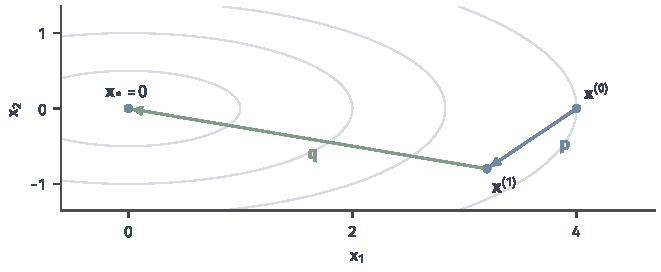
\includegraphics[width=112mm]{figures/01-mathematical-preliminaries-upper/02-linear-spaces/matplotlib/comprehension-additions/linear-conjugate-directions.pdf}
  \caption{共轭方向保留已完成的方向优化。目标为$\phi(\bm x)=\tfrac12(x_1^2+4x_2^2)$，
  灰线为等值线；从$(4,0)^\top$先沿$\bm p=(1,1)^\top$精确线搜索至$(3.2,-0.8)^\top$，
  再沿$\bm q=(-4,1)^\top$到达原点，两方向满足$\bm p^\top\bm A\bm q=0$。本图为解析教学示例。}
  \label{fig:vol1-add-linear-conjugate-directions}
\end{figure}

沿当前方向$\bm p_t$把$\phi$看作步长$\alpha$的一元函数
$\phi(\bm x_t+\alpha\bm p_t)$，展开后对$\alpha$求零点（一维最小化）得
\begin{equation}
 \alpha_t=\frac{\bm p_t^\top\bm r_t}{\bm p_t^\top\bm A\bm p_t}.
\end{equation}
分子是当前方向与残差的配对，分母是方向的能量长度。正定性保证分母
$\bm p_t^\top\bm A\bm p_t>0$，步长合法；若分子为零说明该方向已无改进，
不应再沿它移动。步长不是经验调节参数，而是这一一维最小化的唯一解。

\paragraph{残差正交与方向短递推}

\term{共轭梯度法}（conjugate gradient, CG）从$\bm p_0=\bm r_0$开始：
\begin{align}
 \alpha_t&=\frac{\bm r_t^\top\bm r_t}{\bm p_t^\top\bm A\bm p_t},&
 \bm x_{t+1}&=\bm x_t+\alpha_t\bm p_t,\\
 \bm r_{t+1}&=\bm r_t-\alpha_t\bm A\bm p_t,&
 \beta_t&=\frac{\bm r_{t+1}^\top\bm r_{t+1}}{\bm r_t^\top\bm r_t},\\
 \bm p_{t+1}&=\bm r_{t+1}+\beta_t\bm p_t.&
\end{align}
系数由归纳同时保证三件事：非零残差$\bm r_0,\ldots,\bm r_t$彼此正交；
方向$\bm p_0,\ldots,\bm p_t$彼此$\bm A$共轭；前$t+1$个残差与方向都张成
$\mathcal K_{t+1}$。$t=0$由$\bm p_0=\bm r_0$成立。线搜索使新残差与当前方向
正交；对更早的$j<t$，由$\bm A\bm p_j=(\bm r_j-\bm r_{j+1})/\alpha_j$属于
$\mathcal K_{t+1}$，新残差与之正交，故$\bm r_{t+1}\perp\mathcal K_{t+1}$。
只剩与$\bm p_t$共轭一项需要选$\beta_t$：由新旧残差正交得
$(\bm r_{t+1})^\top\bm A\bm p_t=-\lVert\bm r_{t+1}\rVert_2^2/\alpha_t$，
$(\bm p_t)^\top\bm A\bm p_t=\lVert\bm r_t\rVert_2^2/\alpha_t$，
取$\beta_t=\lVert\bm r_{t+1}\rVert_2^2/\lVert\bm r_t\rVert_2^2$后
$\bm p_{t+1}=\bm r_{t+1}+\beta_t\bm p_t$便与$\bm p_t$共轭，归纳闭合。
$\bm r_t^\top\bm r_t$出现在$\alpha_t$分子，正是因为$(\bm p_t)^\top\bm r_t
=\lVert\bm r_t\rVert_2^2$。

\paragraph{PCG的预条件残差}

\term{预条件共轭梯度}（preconditioned CG, PCG）以对称正定$\bm M$配置预条件，
等价变换系统为$\bm L^{-1}\bm A\bm L^{-\top}\bm z=\bm L^{-1}\bm b$（$\bm M=\bm L\bm L^\top$）。
实现时不解变换坐标，而是每步解$\bm M\bm z_t=\bm r_t$，这里的$\bm z_t$是
预处理后的残差而非变换坐标；初始方向也必须同步改为$\bm p_0=\bm z_0$，
不能只替换迭代中的系数。系数同步改变为
$\alpha_t=\bm r_t^\top\bm z_t/(\bm p_t^\top\bm A\bm p_t)$，
$\beta_t=\bm z_{t+1}^\top\bm r_{t+1}/(\bm z_t^\top\bm r_t)$，
$\bm p_{t+1}=\bm z_{t+1}+\beta_t\bm p_t$。直接把一般非对称左预条件矩阵当作
欧氏对称矩阵是不对的，非对称预条件器不能继承CG的正分母与能量论证。

正定性保证非零方向的$\bm p_t^\top\bm A\bm p_t>0$，分母合法。新残差为零即停止，
不再做含零分母的更新。各次方向更新保证$\bm x_k-\bm x_0\in\mathcal K_k$，
残差与$\mathcal K_k$正交正是该子空间内极小化的一阶条件，正定性又使其充分。
非零共轭方向必线性无关，因此精确算术下至多$d$步得零残差；有限精度下正交性
受损，不能把有限步结论当作实现保证，实际步数与停滞由后续章节说明。
可复算小例子：$\bm A=\operatorname{diag}(1,2)$、$\bm b=(1,1)^\top$、零初值。
第一步$\alpha_0=2/3$得$\bm x^{(1)}=(2/3,2/3)^\top$、
$\bm r^{(1)}=(1/3,-1/3)^\top$，$\beta_0=1/9$给
$\bm p^{(1)}=(4/9,-2/9)^\top$；第二步$\alpha_1=3/4$得
$\bm x^{(2)}=(1,1/2)^\top$，残差恰为零。

每步一次矩阵作用$\bm A\bm p_t$、若干内积（$\bm r_t^\top\bm r_t$、
$\bm p_t^\top\bm A\bm p_t$）与向量更新（$\bm x_{t+1}$、$\bm r_{t+1}$、$\bm p_{t+1}$），
额外存储$O(d)$个向量（当前解、残差、方向；PCG再加预处理残差$\bm z_t$），
不需要形成$\bm A^{-1}$或任何稠密因子。预条件作用、
内积与辅助求解$\bm M\bm z_t=\bm r_t$都计入每步成本；矩阵作用本身按$\bm A$的
非零结构计，稠密与稀疏差别显著。

\subsubsection{MINRES}

\paragraph{对称不定系统与残差目标}

矩阵仍实对称但不正定时，能量范数$\lVert\cdot\rVert_{\bm A}$与正分母失效，
CG的能量最小化论证不能沿用。\term{MINRES}（minimum residual）改在
$\mathcal K_k$中直接最小化原方程残差$\lVert\bm A\bm x-\bm b\rVert_2$，
不要求$\bm A$正定；对称不定性本身不导致不可解，只是不能继续使用CG的
正分母或能量范数论证。

沿用Lanczos短递推构造正交基$\bm V_k$，使
$\bm A\bm V_k=\bm V_{k+1}\bm T_k$，$\bm T_k$为对称三对角（对称使Hessenberg的
次对角与上对角相等，非对角非零项只剩相邻两条）。大系统被压成
逐步更新的小型三对角问题，短递推只需相邻三个向量、不需保存全部基；有限精度下
正交性逐渐损失，必要时重正交化会增加存储与计算。

候选$\bm x=\bm x_0+\bm V_k\bm y$的残差写成$\bm V_{k+1}(\beta\bm e_1-\bm T_k\bm y)$，
其中$\beta=\lVert\bm r_0\rVert_2$；由于$\bm V_{k+1}$列正交，问题化为
\begin{equation}
 \min_{\bm y}\lVert\beta\bm e_1-\bm T_k\bm y\rVert_2.
\end{equation}
这个小型最小二乘用上文的小型QR求解，三对角边界每次只更新一个角，
用Givens旋转逐步完成，无需解大的正规方程。

求得小问题系数$\bm y$后，由$\bm x_k=\bm x_0+\bm V_k\bm y$
恢复解向量；随$\bm V_k$逐列增长，$\bm y$与解都可递推更新，不必每步从头重组。
实现上通常不直接保存$\bm V_k$乘以完整$\bm y$，而是用递推形式更新解向量；
这与CG只保留几个向量不同，MINRES的三对角短递推保留基的投影关系，
恢复路径同样只依赖相邻几列。

预条件仍要求对称正定$\bm M$；投影在$\bm M$内积下进行，
解释的是$\bm M^{-1/2}$尺度下的残差，停止时仍须回到原始残差$\bm b-\bm A\bm x$
核验，不能把变换后残差当作原方程误差。对称不定$\bm A$配上对称正定
（SPD, symmetric positive definite）预条件后，短递推与
三对角结构保持；非对称$\bm M$会破坏三对角对称关系，不满足MINRES前提。

MINRES可扩展到对称奇异相容系统的最小二乘任务，
但一般不保证给出最小欧氏范数代表；它在核方向上的取值仍可能携带自由分量，
选解需另核，MINRES-QLP等变体（专门约束到零空间正交补）不在本节展开。
奇异系统须先判相容（6.2.1），不相容时残差最小化归后续最小二乘任务。

每步一次矩阵作用加少量向量更新，三对角短递推存储与$k$
无关（只需相邻几个向量）；停止以重算的真实原残差$\bm b-\bm A\bm x_k$核验，
递推估计残差在有限精度下可能分离。若 Lanczos 提前出现零余量，说明空间已不变，
应在当前小问题内取残差极小并停止，不对零向量归一化。

\subsubsection{GMRES}
\label{sec:ch06-gmres}

\paragraph{一般系统与Krylov残差目标}

对可逆的一般方阵（无对称性要求），\term{广义最小残差法}（generalized
minimal residual, GMRES）选择
\begin{equation}
 \bm x_k=\argmin_{\bm x\in\bm x_0+\mathcal K_k(\bm A,\bm r_0)}
 \lVert\bm b-\bm A\bm x\rVert_2.
\end{equation}
它放宽的是对称正定要求，不是完全取消结构条件：这里假设$\bm A$可逆；
方法也能用于其他方阵，但其解集与终止结论要另核。

令$\gamma=\lVert\bm r_0\rVert_2>0$，
$\bm v_1=\bm r_0/\gamma$。Arnoldi过程建立正交基$\bm V_k$，满足
$\bm A\bm V_k=\bm V_{k+1}\overline{\bm H}_k$，$\overline{\bm H}_k$为
$(k+1)\times k$上Hessenberg小矩阵。候选$\bm x=\bm x_0+\bm V_k\bm y$的残差为
$\bm V_{k+1}(\gamma\bm e_1-\overline{\bm H}_k\bm y)$，因$\bm V_{k+1}$列正交，
只需解小型最小二乘$\min_{\bm y}\lVert\gamma\bm e_1-\overline{\bm H}_k\bm y\rVert_2$。

小型问题用Givens旋转逐步更新小型QR（见上文Givens旋转），每步只消去
新进入的一行，最后由$\bm x_k=\bm x_0+\bm V_k\bm y$恢复。若第$k$步剩余
长度为零，关系改为$\bm A\bm V_k=\bm V_k\bm H_k$，小问题相应使用
$k\times k$矩阵$\bm H_k$，无需构造不存在的新基向量。可复算小例子：
$\bm A=[1\ 1;0\ 2]$、$\bm b=(0,1)^\top$、零初值。第一步候选$(0,t)^\top$，
残差$(-t,1-2t)^\top$，最小化$t^2+(1-2t)^2$得$t=2/5$，残差范数
$1/\sqrt5$；第二步搜索空间已是$\mathbb R^2$，得精确解$(-1/2,1/2)^\top$。

左预条件$\bm M^{-1}\bm A\bm x=\bm M^{-1}\bm b$最小化
$\lVert\bm M^{-1}(\bm b-\bm A\bm x)\rVert_2$，求解的是变换后残差；
右预条件$\bm A\bm M^{-1}\bm z=\bm b$最小化原系统残差$\lVert\bm b-\bm A\bm x\rVert_2$，
却需把每个搜索方向经$\bm M^{-1}$映回输入。停止时必须说明核验的是哪一个残差，
不能把变换后残差直接当作原方程误差；两种预条件改变的最小化口径不同，结论不可互替。

\paragraph{扩基存储与重启}

第$k$步除一次矩阵作用外，还要把$\bm A\bm v_k$与$k$个基向量逐一做内积正交化，
成本$O(kd)$，基存储$O(kd)$，每次矩阵作用另计；随$k$增长存储线性上升。
\term{重启GMRES}（restarted GMRES, GMRES($m$)）每隔固定$m$步丢弃旧基并从当前
残差重新开始，以把存储压回$O(md)$；代价是放弃已积累的搜索方向。

重启放弃了旧搜索空间中的方向；精确算术下每轮内残差范数
仍不增加（子空间内取最小），但跨轮可能停滞在某一水平，而且不再保证至多$d$步
终止的精确算术保证（旧方向已被丢弃）。何时重启、
重启后是否换预条件，属于策略选择，本节只指出信息损失这一边界；停滞时应改换
预条件或重启参数，而非盲目增加轮次。

一般可逆矩阵在精确算术中至多$d$步终止；若Arnoldi剩余向量提前为零，
当前空间已不变，且可逆性保证精确解已可在$\bm x_0+\mathcal K_k$中取得，
应结束小问题而非继续除以零。停止以重算的真实残差为准，递推残差是否
可信还要结合条件数与后向误差（后续章节）判断。

\subsubsection{BiCGSTAB}

\paragraph{长递推存储与短递推需求}

GMRES的Arnoldi基随步数增长，存储$O(kd)$；
非对称方阵又没有对称三对角的Lanczos短递推（非对称不具备三对角结构）。
\term{BiCGSTAB}（biconjugate gradient stabilized）以两条短递推
换取固定存储，辅助向量数量与每步成本独立于$k$，代价是放弃GMRES的逐步残差
单调最小化保证。

它引入一对互正交的辅助（影子）残差$\tilde{\bm r}$与
双共轭方向，要求$\tilde{\bm r}^\top\bm p_j=0$的双正交条件，不要求欧氏意义下的
A共轭，因而不继承CG的能量论证（没有正定内积保证方向互不干扰）。双共轭条件在
双边（原残差与影子残差）上建立，而非在单一欧氏内积下；影子序列由$\tilde{\bm r}_0$
与转置矩阵$\bm A^\top$生成，与原序列对偶。

双共轭梯度（BiCG）先给出基础校正$\alpha\bm p$，
但其中间残差可能振荡（非正定内积下方向无法保证单调改善）；BiCGSTAB不直接沿用
振荡序列，而在每步基础校正后构造一个局部平稳校正（再沿新方向做一次小残差极小化）
把振荡压平，两个阶段分开。

每步分两个阶段，各一次矩阵作用，实现为固定几个向量的递推，不保存Krylov基矩阵。
第一阶段（BiCG基础校正）：先记$\rho=\tilde{\bm r}^\top\bm r$，
由上一步的$\rho_{\rm prev}$、$\alpha$、$\omega$合成
$\beta=(\rho/\rho_{\rm prev})(\alpha/\omega)$，更新方向
\begin{equation}
 \bm p\leftarrow \bm r+\beta(\bm p-\omega\bm A\bm p),
\end{equation}
再取基础步长
\begin{equation}
 \alpha=\frac{\rho}{\tilde{\bm r}^\top\bm A\bm p},
\end{equation}
把$\alpha\bm p$加到解上，并得中间残差
\begin{equation}
 \bm s=\bm r-\alpha\bm A\bm p.
\end{equation}
第二阶段（局部平稳校正）：在$\bm s$附近沿$\bm A\bm s$方向极小化
$\lVert\bm s-\omega\bm A\bm s\rVert^2$，对$\omega$求零值得
\begin{equation}
 \omega=\frac{\bm s^\top\bm s}{\bm s^\top\bm A\bm s}.
\end{equation}
随后完成本步更新
\begin{equation}
 \bm x\leftarrow\bm x+\alpha\bm p+\omega\bm s,\qquad
 \bm r\leftarrow\bm s-\omega\bm A\bm s,\qquad
 \rho_{\rm prev}\leftarrow\rho,
\end{equation}
方向$\bm p$进入下一步。$\omega$由局部小残差极小化决定，不是经验参数；
完整收敛性、非单调边界与非对称系统的失败模式留第7章，本节只给出可执行更新。

预条件作用在每步辅助求解处插入（解$\bm M\bm z=\bm r$），位置与PCG类似，
但BiCGSTAB本身不要求对称预条件（非对称系统配一般预条件即可）；预条件器改变的是
双正交序列的尺度，不改变方法的非对称性质。

递推有两个关键分母：第一阶段$\alpha$的双共轭分母$\tilde{\bm r}^\top\bm A\bm p$，
第二阶段$\omega$的平稳校正分母$\bm s^\top\bm A\bm s$；任一为零即breakdown，
此时该方向序列无法继续，不能强行代入；近失效（分母极小）
会放大数值误差，应停止并改换方法（如重启GMRES），而非硬除。分母为零属于精确
算术下的结构失效，不是单纯精度问题。

每步约两次矩阵作用与少量内积，不保存Krylov基矩阵，存储为固定个数的向量。
BiCGSTAB不保证残差单调下降（中间可能回升），也没有至多$d$步终止的简单陈述；
结果以重算的真实原残差$\bm b-\bm A\bm x$核验，适用性与失败模式（breakdown、
振荡停滞）归后续章节说明。

\subsection{方法选择与结果核验}

先核验结构判据再选方法：
\begin{enumerate}
 \item 对称正定：优先 Cholesky 或 CG。
 \item 对称不定：MINRES。
 \item 一般方阵（无对称/正定要求，且可逆）：LU 或 GMRES。
 \item 非对称非正定：GMRES 或 BiCGSTAB。
 \item 只能调用$\bm v\mapsto\bm A\bm v$（黑箱）：选 Krylov 方法。
 \item 多右端且矩阵固定：优先复用同一次分解。
\end{enumerate}
对称、正定、稀疏、带状等结构必须先由矩阵本身核验，不能凭方法名称选方法；
目标精度（机器精度级高精度还是宽容限近似）也直接决定直接法与迭代法的取舍：
高精度小系统直接法一步到位，大系统宽容限则迭代法更省。

同任务比较总账：直接法的一次性建立（分解$O(d^3)$）、迭代法的每步成本（矩阵作用
$O(\text{非零元})$）、预条件的辅助求解、存储，以及多右端摊还。不单独按维数或
稀疏性宣布某类方法更快——便宜预条件可能需要更多迭代，贵预条件可能减少步数，
二者相乘（建立$+$每步$\times$步数）才是比较口径。矩阵可整体获得且要求高精度时
直接法核验直接；只能提供矩阵作用或规模极大时迭代法可行，但须把预条件构造计入
总账。

停止一律以原系统残差$\bm b-\bm A\bm x$（按右端或尺度归一）为准，不使用
预条件变换后残差代替；残差小不等于参数准确。解出后回代核验，并复核所选
方法的前提（可逆、正定、非零对角、分母非零）是否满足。条件数、误差放大
与收敛速度由后续扰动与收敛章节报告，本节不提前给阈值。

\section{最小二乘：近似求解}
\label{sec:ls-least-squares}
\label{sec:linear-algebra-residual-systems}
\label{sec:linear-algebra-projection-least-squares}
\label{sec:matrix-analysis-inverse-input-selection}

第~\ref{sec:ls-exact-linear-equations}节要求$\bm A\bm x=\bm b$精确成立，相容性不满足时方程无解。
观测总有误差，方程数也常多于未知数，此时不应再寻找不存在的精确解，而要在所有输入中挑选
使输出误差最小的一个。本节把“误差最小”写成可计算的平方残差目标，分别讨论普通、加权和
正则化三种目标的存在性、唯一性与选解，再给出正规方程、QR、SVD与迭代四类求解路径，
最后说明怎样按矩阵形状、数值尺度和停止准则选择方法并核验结果。灵敏度与收敛速度属于
后续扰动分析与迭代收敛章节，本节只回答目标是什么、解是否存在、怎样更新与核验。

\subsection{残差与目标}
\label{sec:ls-least-squares-objective}

给定$\bm A\in\mathbb R^{m\times d}$和观测$\bm b\in\mathbb R^m$，当不存在$\bm x$使
$\bm A\bm x=\bm b$时，改求使平方输出误差最小的输入：
\begin{equation}
 \min_{\bm x\in\mathbb R^d}\ \lVert\bm A\bm x-\bm b\rVert_2^2.
 \label{eq:linear-algebra-least-squares}
\end{equation}
这一任务称为\term{最小二乘}（least squares）。设计矩阵记号$\bm X\bm w=\bm y$只是同一问题
的回归写法，$\bm X$对应$\bm A$，系数$\bm w$对应$\bm x$，响应$\bm y$对应$\bm b$。
平方误差取欧氏长度的平方，既去掉非负平方根又保持最小点不变，也使目标成为输入的二次函数。

若$\bm b\in\operatorname{range}(\bm A)$，存在输入使残差$\bm r=\bm b-\bm A\bm x$为零，
平方残差的最小值就是$0$；此时最小二乘问题退化为第~\ref{sec:ls-exact-linear-equations}节的
相容精确方程，精确解是最小残差为零的特殊情形，而不是另一种无关的定义。以下讨论集中在
$\bm b$不可达、最小残差严格为正的一般情形。

观测可以同时有若干列。给定$\bm B\in\mathbb R^{m\times n}$，求$\bm X\in\mathbb R^{d\times n}$使
\begin{equation}
 \min_{\bm X}\ \lVert\bm A\bm X-\bm B\rVert_{\mathrm F}^2
 =\sum_{j=1}^n\lVert\bm A\bm x_j-\bm b_j\rVert_2^2,
 \label{eq:ls-multi-right-frobenius}
\end{equation}
其中$\bm b_j$、$\bm x_j$分别是$\bm B$、$\bm X$的第$j$列。Frobenius平方范数把各列残差的
平方长度相加，目标对每一列独立；因此多右端问题就是$n$个同矩阵最小二乘问题并列，分解一次
可以复用于全部列，不存在列间耦合。

不同观测的可靠程度不同，误差代价也不必相同。给定对称正定权重$\bm M\in\mathbb R^{m\times m}$，
\term{加权最小二乘}（weighted least squares）的目标为
\begin{equation}
 \min_{\bm x}\ (\bm A\bm x-\bm b)^\top\bm M(\bm A\bm x-\bm b),
 \label{eq:ls-weighted-objective}
\end{equation}
它等于在$\bm M$内积下度量残差长度，$\bm M$对角元较大的坐标误差被惩罚得更重。权重记录
各输出坐标之间的相对代价，不能与后文惩罚输入幅度的正则化参数混为一谈。若$\bm M$仅半正定，
某些坐标的误差可能被完全忽略，唯一性结论要重新检查，见~\ref{sec:ls-weighted-ls}。

\paragraph{岭回归与一般Tikhonov惩罚}

当矩阵的某些方向几乎不改变输出时，反求的系数会被放大；在数据项之外附加输入幅度的二次惩罚，
得到\term{岭回归}（ridge regression）目标
\begin{equation}
 \min_{\bm x}\ \lVert\bm A\bm x-\bm b\rVert_2^2+\lambda\lVert\bm x\rVert_2^2,
 \qquad \lambda>0.
 \label{eq:ls-ridge-objective}
\end{equation}
更一般地，惩罚可以作用在希望压小的变化量$\bm L\bm x$上，其中$\bm L\in\mathbb R^{p\times d}$
记录这种偏好，得到\term{Tikhonov正则化}（Tikhonov regularization）的一般二次形式
\scite{math-hansen2008regtools}
\begin{equation}
 \min_{\bm x}\ F_\lambda(\bm x)
 =\lVert\bm A\bm x-\bm b\rVert_2^2+\lambda\lVert\bm L\bm x\rVert_2^2,
 \qquad \lambda>0.
 \label{eq:linear-algebra-general-tikhonov}
\end{equation}
$\bm A$记录观测作用，$\bm L$记录要压小的变化，二者行数不必相同；$\bm L=\bm I$时回到岭回归。
惩罚改变的是目标本身，而不是让分解“算得出来”的实现细节：选择$\lambda$是在重新设定任务，
不能仅作为数值技巧解释。

\subsection{存在性、唯一性与选解}
\label{sec:ls-ls-existence}

先在每种目标下回答三个问题：最小点是否存在；若存在，输入是否唯一；不唯一时按什么准则
挑选代表。拟合值$\bm A\bm x$、输入$\bm x$与残差$\bm r$要分别核验，不能互相替代。

\subsubsection{普通最小二乘}
\label{sec:ls-ordinary-ls}

平方残差$\lVert\bm A\bm x-\bm b\rVert_2^2$只通过拟合值$\bm A\bm x$依赖输入：
拟合值遍历列空间$\operatorname{range}(\bm A)$，问题等价于在$\operatorname{range}(\bm A)$中
寻找离$\bm b$最近的点。第~\ref{sec:ls-subspace-nearest-points}节已经证明，有限维子空间中
到给定点的欧氏最近点存在且唯一。

因此最近拟合值$\hat{\bm b}$存在且唯一，与输入是否唯一无关。即便多个输入到达同一个
$\hat{\bm b}$，输出端的选择已经确定。最近点把$\bm b$分解为
$\bm b=\hat{\bm b}+\bm r$，其中$\hat{\bm b}\in\operatorname{range}(\bm A)$，
残差$\bm r$与整个列空间正交。

\paragraph{正交残差与正规方程}

残差与每一列正交，即对任意$\bm x$有$\bm x^\top\bm A^\top\bm r=0$，故
$\bm A^\top\bm r=\bm0$。代入$\bm r=\bm b-\bm A\hat{\bm x}$得到\term{正规方程}
（normal equations）
\begin{equation}
 \bm A^\top(\bm b-\bm A\hat{\bm x})=\bm0,
 \qquad
 \bm A^\top\bm A\hat{\bm x}=\bm A^\top\bm b.
 \label{eq:linear-algebra-normal-equations}
\end{equation}
“正规”来自法向（正交）关系，不是归一化。
图~\ref{fig:ls-least-squares-residual}把这一正交关系画成三维透视：拟合值$\bm A\hat{\bm x}$
落在列空间平面上，残差$\bm r=\bm b-\bm A\hat{\bm x}$与两条列向量都垂直。

\begin{figure}[htbp]
  \centering
  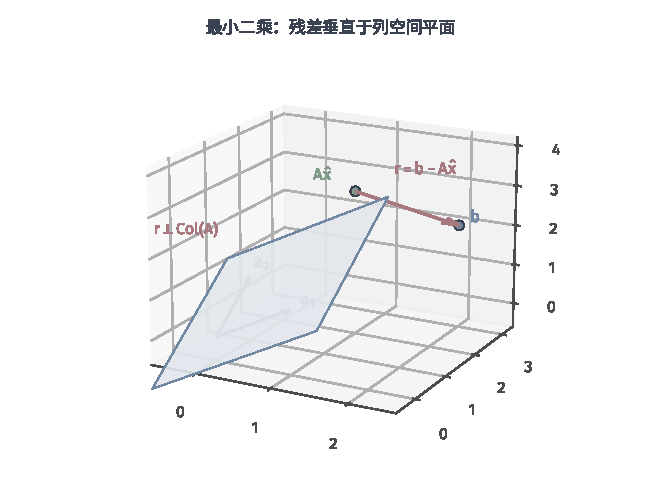
\includegraphics[width=112mm]{figures/01-mathematical-preliminaries-upper/02-linear-spaces/matplotlib/ls-least-squares-residual/ls-least-squares-residual.pdf}
  \caption{列空间平面上的最近点。$\bm A=\left[\begin{smallmatrix}1&0\\0&1\\1&1\end{smallmatrix}\right]$，
  列$\bm a_1=(1,0,1)^\top$、$\bm a_2=(0,1,1)^\top$张成浅蓝平面；$\bm b=(2,3,2)^\top$，
  最近拟合值$\bm A\hat{\bm x}=(1,2,3)^\top$，残差$\bm r=(1,1,-1)^\top$满足
  $\bm r^\top\bm a_1=\bm r^\top\bm a_2=0$。透视教学构造。}
  \label{fig:ls-least-squares-residual}
\end{figure}

正规方程不仅必要，也足以保证全局最小。对任意增量$\bm h$，
\[
 \lVert\bm A(\hat{\bm x}+\bm h)-\bm b\rVert_2^2
 =\lVert\bm A\hat{\bm x}-\bm b\rVert_2^2
 -2\bm h^\top\bm A^\top\bm r+\lVert\bm A\bm h\rVert_2^2.
\]
正规方程使中间项$\bm h^\top\bm A^\top\bm r=\bm h^\top\bm0=0$，剩下非负的
$\lVert\bm A\bm h\rVert_2^2$，故任意移动都不会减小目标。

拟合值唯一不代表输入唯一。若$\hat{\bm x}$是一个解，$\bm z\in\ker\bm A$时
$\bm A(\hat{\bm x}+\bm z)=\hat{\bm b}$不变，所以全部最优输入为
\begin{equation}
 \hat{\bm x}+\ker\bm A.
 \label{eq:ls-all-ordinary-solutions}
\end{equation}
满列秩时$\ker\bm A=\{\bm0\}$，正规矩阵$\bm A^\top\bm A$正定且可逆，唯一输入为
\begin{equation}
 \hat{\bm x}=(\bm A^\top\bm A)^{-1}\bm A^\top\bm b.
 \label{eq:linear-algebra-full-rank-least-squares}
\end{equation}
否则任意零空间增量都不改变目标，输入不唯一。

满列秩只保证系数唯一，不保证系数稳定。贯穿例（设计矩阵~\eqref{eq:linear-algebra-nearly-collinear-design}）
展示两列几乎同向时系数如何被放大。取$\bm c_1=(1,1,1)^\top$、$\bm q=(0,1,-1)^\top$，
两列为$\bm c_1$与$\bm c_1+\varepsilon\bm q$，响应$\bm y=\bm c_1+\delta\bm q$。
正规方程具体为
\[
 \begin{bmatrix}3&3\\3&3+2\varepsilon^2\end{bmatrix}\hat{\bm w}
 =\begin{bmatrix}3\\3+2\varepsilon\delta\end{bmatrix},
\]
系数矩阵行列式为$6\varepsilon^2$。$\varepsilon\neq0$时满列秩，
\begin{equation}
 \hat{\bm w}_\varepsilon
 =\begin{bmatrix}1-\delta/\varepsilon\\\delta/\varepsilon\end{bmatrix},
 \qquad\bm X_\varepsilon\hat{\bm w}_\varepsilon=\bm y,
 \label{eq:linear-algebra-nearly-collinear-least-squares}
\end{equation}
$\varepsilon=0.01$、$\delta=0.1$时系数为$(-9,10)^\top$，残差却为零。
$\varepsilon=0$时两列重合为$\bm c_1$，正交分解$\bm y=\bm c_1+\delta\bm q$的最近输出
为$\bm c_1$，残差为$\delta\bm q$（平方残差$2\delta^2$），全部系数满足$w_1+w_2=1$。
于是矩阵趋于极限时，精确拟合所需的系数发散，而极限矩阵不再能精确拟合：拟合值可以相当
稳定，表示它的两个系数却可能很大。这是近共线几何本身的结果，不是计算机造成的现象。

输入多解时需要额外准则选定代表。要求欧氏范数最小，就是去掉不改变输出的零空间分量：
把$\hat{\bm x}$分解为$(\ker\bm A)^\perp$分量与$\ker\bm A$分量，两项正交，平方范数相加，
最小值只在零空间分量为零时达到。这一选择的显式构造留给伪逆，见~\ref{sec:ls-pseudoinverse}。

\subsubsection{加权最小二乘}
\label{sec:ls-weighted-ls}

加权目标$(\bm A\bm x-\bm b)^\top\bm M(\bm A\bm x-\bm b)$中的$\bm M$对称正定。
它定义输出空间的$\bm M$内积$\langle\bm u,\bm v\rangle_{\bm M}=\bm u^\top\bm M\bm v$，
加权残差在该内积下与列空间正交。

\paragraph{白化后的普通最小二乘}

由~\ref{thm:ls-gram-factor}的配方结论，正定$\bm M$可写成$\bm M=\bm R^\top\bm R$，
其中$\bm R$可逆。令$\tilde{\bm A}=\bm R\bm A$、$\tilde{\bm b}=\bm R\bm b$，则
加权目标等于普通平方残差$\lVert\tilde{\bm A}\bm x-\tilde{\bm b}\rVert_2^2$。
这一步常称\term{白化}（whitening）：先把各坐标误差变换到同一欧氏尺度，再回到已证的
普通问题。正交条件给出加权正规方程
\begin{equation}
 \bm A^\top\bm M(\bm b-\bm A\hat{\bm x})=\bm0,
 \qquad
 \bm A^\top\bm M\bm A\,\hat{\bm x}=\bm A^\top\bm M\bm b.
 \label{eq:linear-algebra-weighted-normal-equations}
\end{equation}

白化后的最近点存在唯一，故加权拟合值$\bm A\hat{\bm x}$存在。满列秩时
$\bm A^\top\bm M\bm A$正定，输入唯一；欠定或列相关时，输入仍沿$\ker\bm A$模糊，
与普通情形同理。

若$\bm M$仅半正定，它可能忽略非零残差：例如$\bm A=\bm I$、$\bm M=\operatorname{diag}(1,0)$
时第二个拟合坐标不受目标约束，任意取值都不改变代价。被$\bm M$消去的输出方向上，
拟合值本身不再唯一，不能直接沿用正定权重的结论。

半正定$\bm M$仍给出半内积，目标在有限维输入上连续；在受约束的方向范围内取到下界，
最小点存在；不可辨认方向构成解集的仿射纤维，可在其中另取欧氏范数最小的代表。
这种选择不恢复被权重消去的信息，只是在等价解中挑一个规范代表。

多右端时若各列共用同一个$\bm M$，各列仍然独立。若不同输出坐标或不同右端列需要不同权重，
把矩阵按列向量化后，权重作用在拉长的残差向量上，列间通过权重矩阵耦合，不能再逐列独立求解。

\subsubsection{正则化最小二乘}
\label{sec:ls-regularized-ls}

一般Tikhonov目标$F_\lambda(\bm x)=\lVert\bm A\bm x-\bm b\rVert_2^2+\lambda\lVert\bm L\bm x\rVert_2^2$
同时衡量数据拟合与惩罚量。两项都非负，$\lambda>0$平衡二者；这不是普通最小二乘的近似，
而是另一个目标。

\paragraph{二次增量与正规算子}

在$\hat{\bm x}$处沿$\bm h$移动，数据项增量为
$\lVert\bm A\bm h\rVert_2^2-2\bm h^\top\bm A^\top(\bm b-\bm A\hat{\bm x})$，
惩罚项增量为$\lambda\lVert\bm L\bm h\rVert_2^2$。一阶项合并为零的条件是
\begin{equation}
 (\bm A^\top\bm A+\lambda\bm L^\top\bm L)\hat{\bm x}=\bm A^\top\bm b.
 \label{eq:ls-tikhonov-normal}
\end{equation}
系数矩阵$\bm A^\top\bm A+\lambda\bm L^\top\bm L$对称，对任意$\bm h$其二次型为
$\lVert\bm A\bm h\rVert_2^2+\lambda\lVert\bm L\bm h\rVert_2^2\geq0$。

二次型为零当且仅当$\bm A\bm h=\bm0$且$\bm L\bm h=\bm0$，即
\begin{equation}
 \ker\bm A\cap\ker\bm L=\{\bm0\}
 \label{eq:linear-algebra-tikhonov-common-nullspace}
\end{equation}
时系数矩阵正定；否则沿公共零空间方向既不改变观测也不改变惩罚，目标对该方向平坦。

正规算子对称，方程有解当且仅当右端$\bm A^\top\bm b$与其零空间正交：对公共零空间中的$\bm z$，
$\bm z^\top\bm A^\top\bm b=(\bm A\bm z)^\top\bm b=0$恒成立，故相容性自动满足，最小点存在。

$\lambda>0$时，若公共零空间为零，系数矩阵正定，增量
$\lVert\bm A\bm h\rVert_2^2+\lambda\lVert\bm L\bm h\rVert_2^2$对$\bm h\neq\bm0$严格为正，
最小点唯一。公共零空间非零时，所有最小点仍相差该空间中的向量，可另取范数最小代表，
正则化并不恢复被两者共同消去的方向。$\bm L=\bm I$时公共零空间自动为零，岭回归因而总有
唯一解；差分惩罚则未必，例如$\bm A=\bm L=[\,1\ -1\,]$时常量方向$(1,1)^\top$
仍在公共零空间中，无论$\lambda$多大都不能确定两个值的共同水平。

$\lambda=0$时目标退回普通最小二乘，唯一性由$\ker\bm A$决定；$\lambda$从正降到零是目标的
连续改变，不是同一问题的参数微调。$\lambda\to\infty$时解趋于$\ker\bm L$中的最小二乘代表，
两端的极限行为在参数选择处再用。

\subsection{直接法}
\label{sec:ls-direct-methods-ls}

直接法把系数矩阵化成可回代的因子。三种路径对应三种矩阵处境：满列秩且规模适中时形成
正规方程；要避免Gram矩阵损失尺度时用QR；秩未知、矩形且需要四个子空间时用SVD。

\subsubsection{正规方程法}
\label{sec:ls-normal-equations-method}

由~\eqref{eq:linear-algebra-normal-equations}，最小二乘解满足对称正规方程
$\bm A^\top\bm A\hat{\bm x}=\bm A^\top\bm b$。这是一个$d$阶对称方阵方程，第~\ref{sec:ls-direct-methods}节
建立的对称正定求解工具可以直接套用。

$\bm A$满列秩时$\bm A^\top\bm A$正定：$\bm x^\top\bm A^\top\bm A\bm x=\lVert\bm A\bm x\rVert_2^2$，
且$\bm A\bm x=0$只在$\bm x=0$时成立。因而正规方程有唯一解，不需要额外选解准则。

对正定$\bm A^\top\bm A$作Cholesky分解$\bm L\bm L^\top$，依次前代求$\bm L\bm z=\bm A^\top\bm b$、
回代求$\bm L^\top\hat{\bm x}=\bm z$，复用第~\ref{sec:ls-direct-methods}节的对称分解流程，
不另立新算法。加权目标对$\bm A^\top\bm M\bm A$、正则化目标对
$\bm A^\top\bm A+\lambda\bm L^\top\bm L$作同样分解，后者正定性由公共零空间条件保证。

稠密矩阵先计算$\bm A^\top\bm A$（约$md^2$次乘法），再作$d^3/3$量级的Cholesky；
多个右端复用同一分解。这一方法只需要矩阵整体可访问，适合小型满列秩问题。

形成$\bm A^\top\bm A$把小的奇异方向平方：接近零的方向被压得更小，浮点中可能直接与零
不可区分。正规方程法只在列之间明显分离、$\bm A^\top\bm A$正定余量充足时可靠；
秩亏或近秩亏时，唯一性本身已经不成立，分解成功也不给出正确选解。条件数放大的定量估计
属于扰动分析，此处只记录这一尺度损失现象。

\subsubsection{QR分解}
\label{sec:ls-qr-method}
\label{sec:linear-algebra-direct-residual}

对$\bm A$作QR分解的构造见第~\ref{sec:ls-orthogonalization-qr}节。正交矩阵保持欧氏长度，
故$\lVert\bm A\bm x-\bm b\rVert_2^2=\lVert\bm Q^\top\bm A\bm x-\bm Q^\top\bm b\rVert_2^2$，
最小点不变。这是QR适合最小二乘的根本原因：只改坐标，不改长度。

瘦QR给出$\bm A=\bm Q\bm R$，$\bm Q$列正交，$\bm R$为上三角。记
$\bm Q^\top\bm b=(\bm c_1,\bm c_2)^\top$、$\bm Q=(\bm Q_1,\bm Q_2)$，则
\[
 \lVert\bm Q\bm R\bm x-\bm b\rVert_2^2
 =\lVert\bm R\bm x-\bm c_1\rVert_2^2+\lVert\bm c_2\rVert_2^2.
\]
$\bm c_2$不依赖$\bm x$，是固定残差；可调部分只由上三角方程决定。

满列秩时$\bm R$满秩，$\bm R\hat{\bm x}=\bm c_1$上三角可直接回代，目标最小值就是
$\lVert\bm c_2\rVert_2^2$。QR不显式形成$\bm A^\top\bm A$，避免正规方程的平方尺度损失，
代价是分解本身的运算量高于Cholesky。

欠定（$m<d$）相容时，QR配合行空间表示可给出最小范数解：解落在$\operatorname{range}(\bm A^\top)$，
正交于$\ker\bm A$。完整的最小范数构造在伪逆处给出，此处只说明QR同样服务于这一选解。

带列主元的QR按接近独立的顺序排列列，使接近零的对角元集中到尾部，从而暴露数值秩。
秩的阈值与噪声尺度有关，见~\ref{sec:ls-method-selection}。

秩亏时取前$r$个主元列回代得到一个基本解，自由方向补零；它是一个合法最优解，但未必
最小范数。核验时同时检查输出残差$\bm b-\bm A\hat{\bm x}$与最优性残差
$\bm A^\top(\bm b-\bm A\hat{\bm x})$，并在需要最小范数时核对$\hat{\bm x}$是否正交于
$\ker\bm A$。

\subsubsection{SVD分解}
\label{sec:ls-svd}

QR只处理满列秩或秩揭示的情形；秩未知、矩形矩阵需要同时给出非零方向、零方向、四个子空间
和稳定选解时，使用奇异值分解。它的存在性不能假设：下面先用实对称谱引理从单位球极值
直接构造，这也是全卷首次建立谱定理，后续球面极值、低秩逼近与矩阵函数都复用这一结论。

对任意$\bm A\in\mathbb R^{m\times d}$，希望找到两组正交方向，使$\bm A$在其间只作独立
伸缩。这需要先证明\term{谱定理}（spectral theorem）：对称矩阵能在正交基下对角化。

\begin{lemma}[实对称谱引理]
\label{thm:ls-real-symmetric-spectral}
\label{thm:matrix-analysis-symmetric-spectral-theorem}
\label{sec:ch06-triangular-spectrum}
设$\bm S\in\mathbb R^{d\times d}$满足$\bm S=\bm S^\top$。存在正交矩阵$\bm Q$与实对角
$\Lambda=\operatorname{diag}(\lambda_1,\dots,\lambda_d)$，使
\begin{equation}
 \bm S=\bm Q\Lambda\bm Q^\top,
 \qquad \bm S\bm q_i=\lambda_i\bm q_i.
 \label{eq:matrix-analysis-symmetric-eigendecomposition}
\end{equation}
对任意$\bm x=\sum_i c_i\bm q_i$，二次型展开为
\begin{equation}
 \bm x^\top\bm S\bm x=\sum_{i=1}^d\lambda_i c_i^2.
 \label{eq:matrix-analysis-quadratic-spectral-form}
\end{equation}
\end{lemma}

\begin{proof}
单位球面$\{\bm x:\lVert\bm x\rVert_2=1\}$是$\mathbb R^d$中的闭有界集，二次型
$q(\bm x)=\bm x^\top\bm S\bm x$连续，由~\ref{thm:ls-extreme-value}在球上取到最大值
$\lambda_1$，记最大点为$\bm q_1$，$\lVert\bm q_1\rVert_2=1$。实对称保证
$\lambda_1=\bm q_1^\top\bm S\bm q_1$是实数。

任取与$\bm q_1$正交的$\bm h$，实数$t$很小时$\bm q_1+t\bm h$归一化后仍在球上，
故其二次型不超过$\lambda_1$倍范数平方。展开：
\[
 \lambda_1+2t\bm h^\top\bm S\bm q_1+t^2\bm h^\top\bm S\bm h
 \leq\lambda_1(1+t^2\lVert\bm h\rVert_2^2).
\]
两边减去$\lambda_1$，$t$的一阶项$2t\bm h^\top\bm S\bm q_1$必须对正负$t$同时不破坏
不等式，因而只能为零，即$\bm h^\top\bm S\bm q_1=0$。对所有$\bm h\perp\bm q_1$成立，
说明$\bm S\bm q_1$没有正交分量，只能平行于$\bm q_1$，即$\bm S\bm q_1=\lambda_1\bm q_1$。
全程只用有限代数增量，不引入复特征多项式。

对$\bm h\perp\bm q_1$，$\bm q_1^\top\bm S\bm h=(\bm S\bm q_1)^\top\bm h
=\lambda_1\bm q_1^\top\bm h=0$，故$\bm S$把$\bm q_1^\perp$映到自身，限制仍是对称矩阵。
在$d-1$维正交补上重复同一极值构造，得到$\bm q_2,\lambda_2$；归纳到一维即得正交列
$\bm q_1,\dots,\bm q_d$与实特征值$\lambda_i$。代入$\bm x=\sum_i c_i\bm q_i$交叉项为零，
便得到谱展开式。这一证明只依赖球的紧性与对称配对，是实情形的完整谱定理；复Hermitian
情形的共轭转置推广在矩阵函数章再给。
\end{proof}

令$\bm S=\bm A^\top\bm A$，它对称且半正定：$\bm x^\top\bm A^\top\bm A\bm x
=\lVert\bm A\bm x\rVert_2^2\geq0$。由谱引理，存在标准正交的$\bm v_i$使
$\bm A^\top\bm A\bm v_i=\lambda_i\bm v_i$，且$\lambda_i\geq0$。记正特征值为
$\sigma_i^2=\lambda_i>0$（$i=1,\dots,r$），$\sigma_i>0$，按降序排列；其余$\bm v_j$满足
$\bm A^\top\bm A\bm v_j=0$，因而$\bm A\bm v_j=0$。

对$\sigma_i>0$定义$\bm u_i=\bm A\bm v_i/\sigma_i$。它们标准正交：
\[
 \bm u_i^\top\bm u_j
 =\frac{\bm v_i^\top\bm A^\top\bm A\bm v_j}{\sigma_i\sigma_j}
 =\frac{\sigma_i^2\delta_{ij}}{\sigma_i\sigma_j}=\delta_{ij}.
\]
且$\bm A\bm v_i=\sigma_i\bm u_i$。

$\bm v_{r+1},\dots,\bm v_d$是$\ker\bm A$的标准正交基；把$\bm u_1,\dots,\bm u_r$扩充为
$\mathbb R^m$的标准正交基，多余方向落在$\operatorname{range}(\bm A)^\perp$。于是
$\bm A$写成秩一矩阵之和
\begin{equation}
 \bm A=\sum_{i=1}^r\sigma_i\bm u_i\bm v_i^\top.
 \label{eq:matrix-analysis-svd-rank-one-sum}
\end{equation}
其中$r=\operatorname{rank}\bm A$，非零奇异值个数就是秩。

\begin{theorem}[SVD的存在与构造]
\label{thm:ls-svd-existence}
对任意$\bm A\in\mathbb R^{m\times d}$，上述构造给出正交$\bm U\in\mathbb R^{m\times m}$、
$\bm V\in\mathbb R^{d\times d}$与对角$\Sigma\in\mathbb R^{m\times d}$，非负对角元
$\sigma_i$使$\bm A=\bm U\Sigma\bm V^\top$。
\end{theorem}

\begin{definition}[奇异值分解]
\label{def:matrix-analysis-svd}
称
\begin{equation}
 \bm A=\bm U\Sigma\bm V^\top
 \label{eq:matrix-analysis-svd}
\end{equation}
为\term{奇异值分解}（singular value decomposition, SVD），非负对角元$\sigma_i$为
\term{奇异值}（singular value），$\bm u_i$、$\bm v_i$分别为左、右\term{奇异向量}
（singular vector）。
\end{definition}

图~\ref{fig:ls-svd-construction}把这一构造拆成三步：先形成对称$\bm A^\top\bm A$，
再由谱引理正交对角化取特征值，最后开方得奇异值、并由$\bm u_i=\bm A\bm v_i/\sigma_i$
得左奇异向量。

\begin{figure*}[htbp]
  \centering
  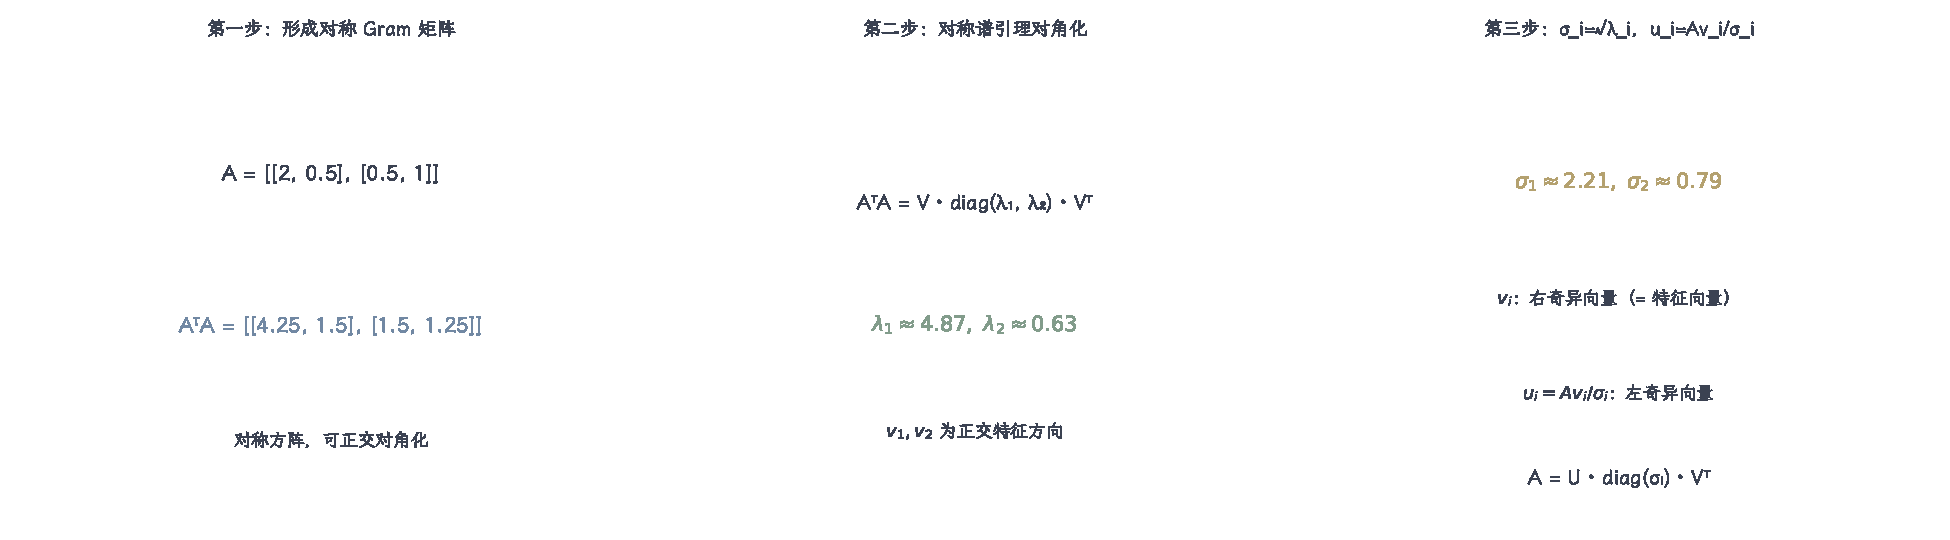
\includegraphics[width=168.998mm]{figures/01-mathematical-preliminaries-upper/02-linear-spaces/matplotlib/ls-svd-construction/ls-svd-construction.pdf}
  \caption{SVD 构造三部曲。以$\bm A=\left[\begin{smallmatrix}2&0.5\\0.5&1\end{smallmatrix}\right]$为例：
  (1)形成$\bm A^\top\bm A=\left[\begin{smallmatrix}4.25&1.5\\1.5&1.25\end{smallmatrix}\right]$；
  (2)对称谱引理对角化，特征值$\lambda_1\approx4.87,\lambda_2\approx0.63$；
  (3)$\sigma_i=\sqrt{\lambda_i}\approx2.21,0.79$，右奇异向量$\bm v_i$即特征向量，
  左奇异向量$\bm u_i=\bm A\bm v_i/\sigma_i$。解析式教学构造。}
  \label{fig:ls-svd-construction}
\end{figure*}

图~\ref{fig:matrix-analysis-svd-geometry}使用二维旋转矩阵
$\bm R(\theta)=
\left[\begin{smallmatrix}\cos\theta&-\sin\theta\\\sin\theta&\cos\theta\end{smallmatrix}\right]$
构造一个左右方向不同的变换，两侧采用相同比例便于比较伸缩量。

\begin{figure*}[htbp]
  \centering
  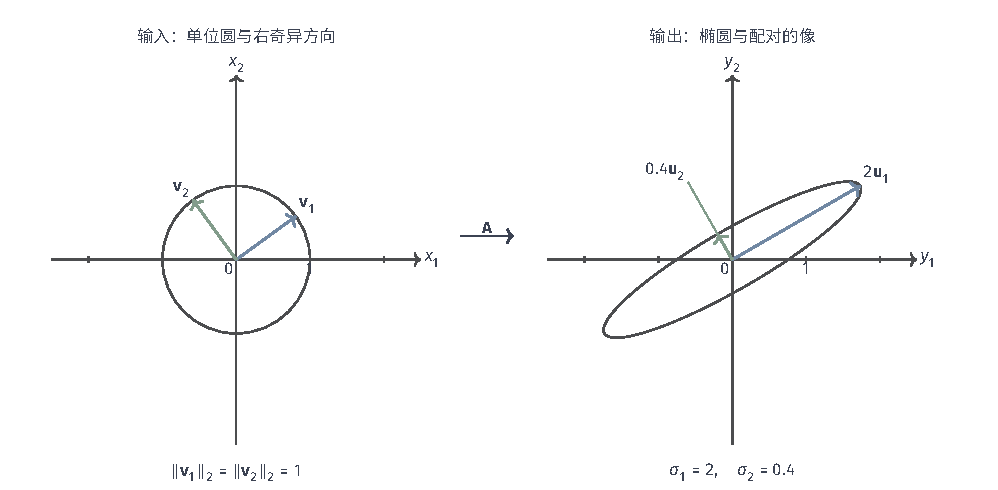
\includegraphics[width=168.998mm]{figures/01-mathematical-preliminaries-upper/02-linear-spaces/tikz/matrix-analysis-svd-geometry/figure.pdf}
  \caption{矩阵$\bm A=\bm R(\pi/6)\operatorname{diag}(2,0.4)\bm R(\pi/5)^\top$
  将单位圆变为椭圆。蓝、绿分别对应两个奇异方向；同色箭头在左侧标出$\bm v_i$，
  在右侧标出其像$\sigma_i\bm u_i$。两侧坐标比例相同。奇异值决定长度变化，左右方向可以不同，
  因而这不是沿特征方向的同空间缩放。图为教学构造。}
  \label{fig:matrix-analysis-svd-geometry}
\end{figure*}

与这一“单位圆变椭圆”的输入侧视角互补，图~\ref{fig:ls-svd-ellipse-action}从行图像与
列图像两侧看最小二乘解：左图两条方程直线交于$\hat{\bm x}=(1,1)^\top$，残差二次型的
水平集是以它为中心的同心椭圆；右图$\bm b$恰落在列空间内，残差为零。

\begin{figure*}[htbp]
  \centering
  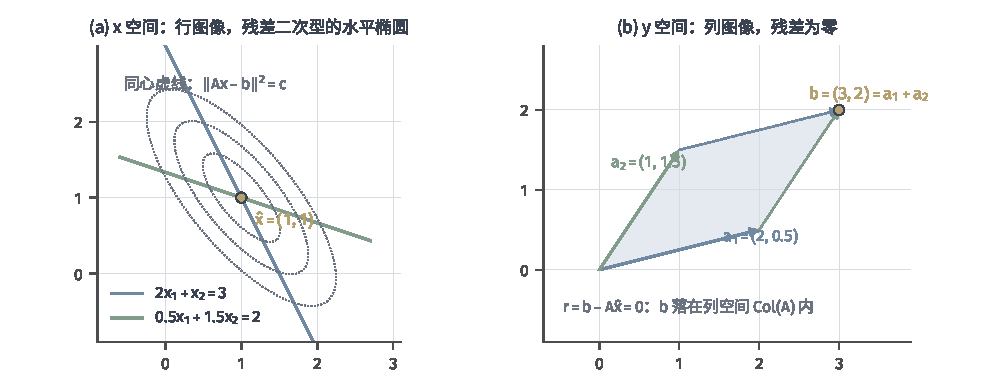
\includegraphics[width=168.998mm]{figures/01-mathematical-preliminaries-upper/02-linear-spaces/matplotlib/ls-svd-ellipse-action/ls-svd-ellipse-action.pdf}
  \caption{最小二乘解的行图像与列图像。$\bm A=\left[\begin{smallmatrix}2&1\\0.5&1.5\end{smallmatrix}\right]$、
  $\bm b=(3,2)^\top$，$\bm A\hat{\bm x}=\bm b$恰有解$\hat{\bm x}=(1,1)^\top$。左：两条方程直线
  交于$\hat{\bm x}$，灰色点线为残差平方$f(\bm x)=\lVert\bm A\bm x-\bm b\rVert_2^2$的水平集，
  中心即交点；右：列$\bm a_1=(2,0.5)^\top$、$\bm a_2=(1,1.5)^\top$张成列空间，
  $\bm b=\bm a_1+\bm a_2$落在其中，残差为零。解析式教学构造。}
  \label{fig:ls-svd-ellipse-action}
\end{figure*}

$\sigma_i$相同时，对应子空间内的任意标准正交旋转仍给出分解，故$\bm U,\bm V$不唯一；
奇异值本身由$\bm A$唯一确定。零奇异值对应的方向不参与伸缩。

数值实现先以Householder双边约化把矩阵变成上双对角形（复用~\ref{sec:ls-orthogonalization-qr}
的反射工具），再用隐式QR位移迭代得到对角元；直接对$\bm A^\top\bm A$求特征值会重蹈
平方尺度损失，故实现始终作用在原矩阵上。

以贯穿例的二维约化看清两个尺度。把设计的输出限制到$\operatorname{span}\{\bm c_1,\bm q\}$，
用$\bm c_1/\sqrt3$、$\bm q/\sqrt2$作正交坐标，再将全部输出统一除以$\sqrt3$，
得到二维表示
\begin{equation}
 \bm X_{\widetilde\varepsilon}
 =\begin{bmatrix}1&1\\0&\widetilde\varepsilon\end{bmatrix},
 \qquad \widetilde\varepsilon=\sqrt{2/3}\,\varepsilon.
 \label{eq:matrix-analysis-nearly-collinear-design}
\end{equation}
这一统一缩放把奇异值除以$\sqrt3$，不改变它们的比值。二维Gram矩阵为
$\bm G_{\widetilde\varepsilon}
=\begin{bmatrix}1&1\\1&1+\widetilde\varepsilon^2\end{bmatrix}$，
其两个特征值由二次方程得到
\begin{equation}
 \lambda_\pm
 =\frac{2+\widetilde\varepsilon^2
          \mathbin{\pm}\sqrt{4+\widetilde\varepsilon^4}}{2},
 \label{eq:matrix-analysis-nearly-collinear-gram-eigenvalues}
\end{equation}
对$\widetilde\varepsilon>0$，$\sigma_\pm=\sqrt{\lambda_\pm}$；
$\widetilde\varepsilon\to0$时$\sigma_{\max}\to\sqrt2$、
$\sigma_{\min}\sim\widetilde\varepsilon/\sqrt2$。大方向近似为两个系数一起变化，
小方向近似为两个系数相消。这一推导只用于理解谱；为计算小奇异值不应显式形成Gram矩阵，
也不宜用相近两数相减求$\lambda_-$，定量原因留给扰动章节。

完整SVD给出$\bm U,\bm V$全正交基；只需要前$k$个奇异方向时可计算薄分解，省去尾部。
稠密完整分解的运算量高于QR，但其明示全部奇异值、四个子空间与最小二乘选解，是秩未知
矩形矩阵的通用工具。

\subsubsection{伪逆与全部最优解}
\label{sec:ls-pseudoinverse}

先看一个欠定小例。$\bm A=[2\ 0]$把$(x_1,x_2)^\top$映成$2x_1$，取$\bm b=(3)$：
方程$2x_1=3$的全部解为$(3/2,t)^\top$，$t$任意，输出只由$x_1$决定。
范数平方$(3/2)^2+t^2$在$t=0$时最小，代表点$(3/2,0)^\top$——它自动落在
$\operatorname{range}(\bm A^\top)$方向上、把零空间分量压为零。伪逆就是把“全部解中
范数最小者”写成一个矩阵的规则：本例$\bm A^\dagger=(1/2,0)^\top$，
$\bm A^\dagger\bm b=(3/2,0)^\top$。下面用SVD把这一规则推广到任意秩。

在$\bm v_i$方向上$\bm A$以$\sigma_i$伸缩到$\bm u_i$，反向自然除以$\sigma_i$：
$\bm u_i\mapsto\bm v_i/\sigma_i$。把$\bm b$按$\bm u_i$展开，可恢复分量
$(\bm u_i^\top\bm b)/\sigma_i$配给$\bm v_i$；落在$\operatorname{range}(\bm A)^\perp$的
分量没有原像，直接丢弃；零方向$\bm v_{r+1},\dots$上$\bm A$没有输出，反向不定义。
小$\sigma_i$在正向作用中压缩，反求时把该分量放大，这是伪逆对弱方向敏感的来源，定量
放大分析属扰动章节。

\begin{definition}[Moore--Penrose伪逆]
\label{def:matrix-analysis-pseudoinverse}
在两端标准内积下，\term{Moore--Penrose伪逆}（Moore--Penrose pseudoinverse）先把
输出正交投影到$\operatorname{range}(\bm A)$，再在$(\ker\bm A)^\perp$上反演：
\[
 \bm A^\dagger=(\bm A|_{(\ker\bm A)^\perp})^{-1}P_{\operatorname{range}(\bm A)}.
\]
用~\ref{thm:ls-svd-existence}的SVD写出即
\begin{equation}
 \bm A^\dagger=\sum_{i=1}^r\frac{1}{\sigma_i}\bm v_i\bm u_i^\top,
 \label{eq:matrix-analysis-pseudoinverse}
\end{equation}
它在$\operatorname{range}(\bm A)^\perp$上取零；$\bm A=\bm0$时定义$\bm A^\dagger=\bm0$。
普通逆是伪逆在可逆方阵上的特殊情形。
\end{definition}

\begin{theorem}[最小二乘与最小范数]
\label{thm:matrix-analysis-pseudoinverse-minimum-norm}
给定$\bm A\in\mathbb R^{m\times d}$和$\bm b\in\mathbb R^m$，全部最小二乘解为
$\bm A^\dagger\bm b+\ker\bm A$，其中$\bm A^\dagger\bm b$是唯一的最小欧氏范数解；
方程相容时它就是全部精确解中的最小范数者。
\begin{proof}
记$P_R$为到$\operatorname{range}\bm A$的正交投影。把
$\bm b=P_R\bm b+\bm b_\perp$（$\bm b_\perp\perp\operatorname{range}\bm A$）、
$\bm x=\bm x_\perp+\bm x_N$（$\bm x_N\in\ker\bm A$）正交分解，则
\[
 \lVert\bm A\bm x-\bm b\rVert_2^2
 =\lVert\bm A\bm x_\perp-P_R\bm b\rVert_2^2+\lVert\bm b_\perp\rVert_2^2.
\]
第二项不能由输入改变；第一项在且仅在$\bm x_\perp$等于投影反演
$(\bm A|_{(\ker\bm A)^\perp})^{-1}P_R\bm b$，也就是$\bm A^\dagger\bm b$时为零。
故全部最优输入为$\bm A^\dagger\bm b+\bm x_N$。两项正交，
$\lVert\bm x\rVert_2^2=\lVert\bm A^\dagger\bm b\rVert_2^2+\lVert\bm x_N\rVert_2^2$，
最小值仅在$\bm x_N=0$时达到。相容时$\bm b_\perp=0$，同一证明适用。
\end{proof}
\end{theorem}

\paragraph{Penrose条件的逐项验证}

由SVD和式直接相乘逐项核对四条：
\begin{enumerate}
 \item $\bm A\bm A^\dagger\bm A=\bm A$；
 \item $\bm A^\dagger\bm A\bm A^\dagger=\bm A^\dagger$；
 \item $(\bm A\bm A^\dagger)^\top=\bm A\bm A^\dagger$；
 \item $(\bm A^\dagger\bm A)^\top=\bm A^\dagger\bm A$。
\end{enumerate}
前两项保证在可反演部分上一致，后两条说明
$\bm A\bm A^\dagger$是到$\operatorname{range}(\bm A)$的正交投影、
$\bm A^\dagger\bm A$是到$(\ker\bm A)^\perp$的正交投影。

满足同样四条的矩阵唯一：若$\bm G$也满足，则$\bm A\bm G=P_R$、$\bm G\bm A=P_{(\ker\bm A)^\perp}$，
于是$\bm G=\bm G\bm A\bm G=P_{(\ker\bm A)^\perp}\bm A^\dagger=\bm A^\dagger$。
故伪逆不由SVD写法决定，是矩阵本身的性质。

$\bm A\bm A^\dagger=\sum_i\bm u_i\bm u_i^\top=P_{\operatorname{range}(\bm A)}$，
$\bm A^\dagger\bm A=\sum_i\bm v_i\bm v_i^\top=P_{(\ker\bm A)^\perp}$；
$\operatorname{range}(\bm A^\dagger)=(\ker\bm A)^\perp$，
$\ker(\bm A^\dagger)=\operatorname{range}(\bm A)^\perp$。四个子空间分属输入端与输出端，
与伴随的正交补关系一致。

例如$\bm A=\begin{smallmatrix}1&1\\0&0\end{smallmatrix}$、$\bm b=(2,1)^\top$，
可达输出只有第二坐标为零的$(2,0)^\top$，残差$(0,1)^\top$无法消除；原像直线
$x_1+x_2=2$上平方范数为$2+2t^2$，伪逆选择$t=0$得到$(1,1)^\top$。伪逆没有使
原本无解的方程突然可解，也没有恢复被$\bm A$消去的信息。

\begin{figure*}[htbp]
  \centering
  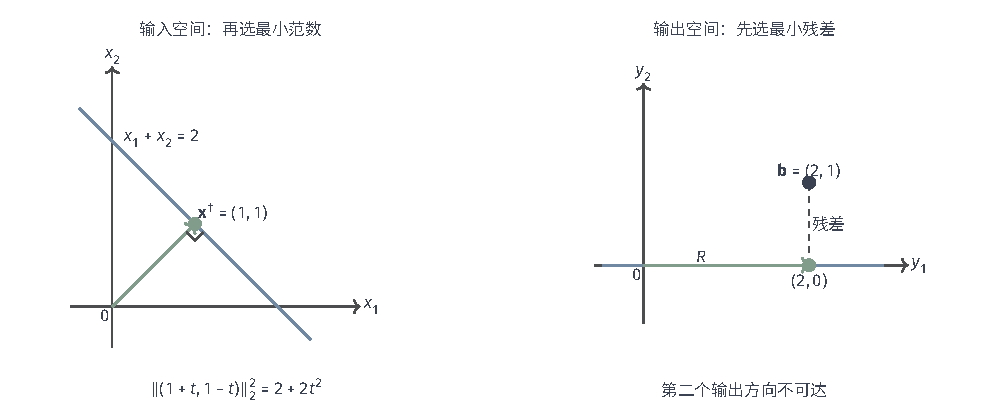
\includegraphics[width=168.998mm]{figures/01-mathematical-preliminaries-upper/02-linear-spaces/tikz/matrix-analysis-pseudoinverse-selections/figure.pdf}
  \caption{伪逆的两次选择。右图先在可达输出中选择离$\bm b=(2,1)^\top$最近的
  $(2,0)^\top$；左图再在整条原像直线$x_1+x_2=2$上选择最靠近原点的$(1,1)^\top$。
  两图属于不同空间，各自等比例绘制。}
  \label{fig:matrix-analysis-pseudoinverse-selections}
\end{figure*}

全部最优输入为
\begin{equation}
 \hat{\bm x}=\bm A^\dagger\bm b+\bm z,
 \qquad \bm z\in\ker\bm A.
 \label{eq:ls-all-pseudoinverse-solutions}
\end{equation}
由证明中的正交分解，$\bm z=0$时范数最小。这就完成了~\ref{sec:ls-ordinary-ls}节
承诺的选解构造。

满列秩时$\bm A^\dagger=(\bm A^\top\bm A)^{-1}\bm A^\top$；满行秩时
$\bm A^\dagger=\bm A^\top(\bm A\bm A^\top)^{-1}$，用于相容欠定系统的最小范数恢复。
任意秩直接用SVD和式，不要套用只在满秩成立的逆公式；伪逆对矩阵不连续（非零标量
$\varepsilon$的伪逆为$1/\varepsilon$，零标量的伪逆为零），秩改变是必须检查的边界。

对~\eqref{eq:ls-multi-right-frobenius}，矩阵最优解为$\bm A^\dagger\bm B$，各列独立取伪逆；
最小范数选解逐列一致，不存在列间耦合。

\subsubsection{加权与正则化的求解}
\label{sec:ls-weighted-regularized-solve}

由$\bm M=\bm R^\top\bm R$把加权问题变成普通最小二乘：$\tilde{\bm A}=\bm R\bm A$、
$\tilde{\bm b}=\bm R\bm b$后，对$\tilde{\bm A}$使用前述QR或SVD，结果代回原变量即得
加权解，不必重造适合$\bm M$的分解。

Tikhonov目标写成普通最小二乘的\term{增广最小二乘}（augmented least squares）形式：
\begin{equation}
 \begin{bmatrix}\bm A\\ \sqrt{\lambda}\,\bm L\end{bmatrix}\bm x
 \approx\begin{bmatrix}\bm b\\ \bm0\end{bmatrix}.
 \label{eq:ls-augmented-system}
\end{equation}
增广矩阵的正规方程正是~\eqref{eq:ls-tikhonov-normal}，故所有普通最小二乘工具原样复用，
不引入新求解器。

若已有$\bm A$的SVD$\bm A=\bm U\Sigma\bm V^\top$且$\bm L=\bm I$，岭解在奇异坐标中为
\begin{equation}
 \hat{\bm x}_\lambda=\sum_{i=1}^r\frac{\sigma_i}{\sigma_i^2+\lambda}
 \bm v_i(\bm u_i^\top\bm b),
 \label{eq:matrix-analysis-ridge-filter-factor}
\end{equation}
每个方向被$\sigma_i/(\sigma_i^2+\lambda)$收缩；小$\sigma_i$方向的放大被压回。
这一收缩改变了解的偏差，其定量放大与偏差分析属于扰动章节，此处只记录表达式。

白化或增广得到的是变换后坐标，必须代回$\bm x$并在原目标中核验：普通项
$\lVert\bm A\hat{\bm x}-\bm b\rVert_2^2$、惩罚项$\lambda\lVert\bm L\hat{\bm x}\rVert_2^2$
与正规方程残差三者分别检查，不能只报变换空间中的残差。

半正定$\bm M$或公共零空间非零时，增广系统在不可辨认方向上仍无唯一解，需另取最小范数
代表；此时不要指望$\lambda$或权重本身恢复被消去的方向。

\subsection{迭代法}
\label{sec:ls-least-squares-iterative}

矩阵只以“给向量返回乘积”的形式给出、或分解填充远超原矩阵时，不构造因子，用序列逼近。
本节只给更新、执行条件与核验量；误差随步数下降的速率证明属于迭代收敛章节。

\subsubsection{Landweber迭代}
\label{sec:ls-landweber}
\label{sec:linear-algebra-gradient-residual}

残差$\bm r=\bm b-\bm A\bm w$沿输出空间；把它搬回输入端的方向是$\bm A^\top\bm r$，
它正是正规方程残差$\bm A^\top\bm b-\bm A^\top\bm A\bm w$。这一伴随作用不需要显式矩阵。

沿$\bm g=\bm A^\top(\bm A\bm w-\bm b)$移动一步，目标增量的一阶项为负；要保证每步不反弹，
步长须使最大伸缩方向的更新倍率绝对值小于$1$，即$0<\eta<2/\lVert\bm A\rVert_2^2$，
其中$\lVert\bm A\rVert_2=\sigma_1$为最大奇异值，由~\ref{thm:ls-svd-existence}的谱定义。

\paragraph{Landweber更新和步长}
\begin{equation}
 \bm w^{(t+1)}=\bm w^{(t)}+\eta\bm A^\top(\bm b-\bm A\bm w^{(t)}),
 \qquad 0<\eta<\frac{2}{\sigma_1^2}.
 \label{eq:ch06-least-squares-gradient-update}
\end{equation}
每步一次$\bm A$作用和一次$\bm A^\top$作用，不形成$\bm A^\top\bm A$。

$\ker\bm A$中的分量不被$\bm A^\top$读取，迭代始终保留初值在$\ker\bm A$中的部分；
零初值收敛到最小范数解，非零初值则保留其零空间分量。收敛证明与极限形式留待收敛章节。

每步核验两个量：输出残差$\bm r^{(t)}=\bm b-\bm A\bm w^{(t)}$与最优性残差
$\bm g^{(t)}=\bm A^\top\bm r^{(t)}$；前者衡量拟合，后者衡量正规方程。每步代价为两次
矩阵向量乘积加若干内积，存储只需要几个向量。

\subsubsection{CGLS迭代}
\label{sec:ls-cgls}

CGLS把共轭梯度法用于正规方程$\bm A^\top\bm A\bm w=\bm A^\top\bm b$，但只在
$\operatorname{range}(\bm A^\top)$内展开，正规方程的CG框架复用第~\ref{sec:ls-krylov-methods}节，
不重复证明有限步终止与正交性。

搜索方向与残差只通过$\bm A\bm p$、$\bm A^\top\bm r$两次乘积更新，从不显式形成
$\bm A^\top\bm A$，因而避免正规算子的平方尺度损失，也不要求矩阵整体存储；只要能给出
正向与伴随乘积，CGLS即可执行。

\paragraph{CGLS的残差和方向更新}

取$\bm w^{(0)}$，$\bm r^{(0)}=\bm b-\bm A\bm w^{(0)}$，$\bm g^{(0)}=\bm A^\top\bm r^{(0)}$，
$\bm p^{(0)}=\bm g^{(0)}$；每步按CG系数更新
\[
 \alpha=\frac{(\bm g^{(t)})^\top\bm g^{(t)}}{(\bm p^{(t)})^\top\bm A^\top\bm A\bm p^{(t)}},
 \quad
 \bm w^{(t+1)}=\bm w^{(t)}+\alpha\bm p^{(t)},
 \quad
 \bm r^{(t+1)}=\bm r^{(t)}-\alpha\bm A\bm p^{(t)},
\]
\[
 \bm g^{(t+1)}=\bm A^\top\bm r^{(t+1)},\qquad
 \beta=\frac{(\bm g^{(t+1)})^\top\bm g^{(t+1)}}{(\bm g^{(t)})^\top\bm g^{(t)}},
 \qquad
 \bm p^{(t+1)}=\bm g^{(t+1)}+\beta\bm p^{(t)}.
\]
分母中的$\bm A^\top\bm A\bm p$以两次乘积实现。

CG只在$\operatorname{range}(\bm A^\top)$内展开搜索空间，零初值且$\ker\bm A$非零时，
迭代自然停在该子空间，给出最小范数解；非零初值保留其$\ker\bm A$分量，不会被算法擦除，
与Landweber相同。要最小范数代表就从$\bm w^{(0)}=\bm0$起步。

以$\lVert\bm g^{(t)}\rVert_2$达到容限为主停止量，同时重算原始残差$\bm r^{(t)}$核验，
不用递推残差直接判定。每步两次乘积、三个方向向量，存储随步数不线性增长。

\subsubsection{LSQR迭代}
\label{sec:ls-lsqr}

CGLS作用在正规算子$\bm A^\top\bm A$上，继承其尺度；LSQR直接在原最小二乘问题上工作，
交替从输出端和输入端投影，适合正规算子病态而原问题本身可解的情形。它同样只调用
$\bm A$与$\bm A^\top$，不显式形成平方矩阵。

从$\bm u_1=\bm b/\lVert\bm b\rVert_2$出发，反复交替用$\bm A^\top$把当前输出方向
映回输入端、再用$\bm A$映回输出端，每步把新方向正交化并归一化，逐步把$\bm A$投影成
下双对角小矩阵；全过程只调用$\bm A$与$\bm A^\top$，不显式形成正规算子。

$k$步后基中系数$\bm z_k$满足等价的小规模最小二乘
\[
 \min_{\bm z_k}\ \lVert\beta_1\bm e_1-\bar{\bm B}_k\bm z_k\rVert_2,
\]
双对角小矩阵维数仅$k$，可用QR直接求解，避免在原空间做大分解。

$\bm w^{(k)}$由输入端基$\bm v_j$按$\bm z_k$的系数线性组合恢复；解不必显式累加全部基，
可用递推公式边走边更新，存储量由实现控制。

零初值在$\operatorname{range}(\bm A^\top)$内逼近最小范数解；秩亏时停止步与容限共同
决定截取哪些方向，过早停止起隐式正则化作用，这一现象的定量分析属扰动章节。

LSQR直接掌握原始残差$\bm b-\bm A\bm w^{(k)}$，核验时重算该残差与$\bm A^\top$投影，
不依赖递推；每步两次乘积加一个双对角小问题求解，基存储随$k$增加，实际使用常配合重启。

\subsubsection{加权与正则化的迭代}
\label{sec:ls-iterative-reuse}

加权问题先白化：正向$\tilde{\bm A}\bm x=\bm R\bm A\bm x$，伴随为$\bm A^\top\bm R^\top$；
对白化后的普通问题跑上述迭代，代价只是把乘积换成加权作用。

正则化增广算子$\begin{bmatrix}\bm A\\\sqrt{\lambda}\bm L\end{bmatrix}$的正向作用拼接
$\bm A\bm x$与$\sqrt{\lambda}\bm L\bm x$，伴随作用拼接$\bm A^\top\bm u$与
$\sqrt{\lambda}\bm L^\top\bm v$，迭代法照用，不需要显式构造增广矩阵。

Landweber、CGLS、LSQR都不依赖具体矩阵元素，只要求可计算正向与伴随乘积。因此把加权
或正则化看成一个新算子后，更新格式、停止量与存储结构原样复用，加权、正则化是换算子，
不是换算法。

停止判定必须回到原目标：加权残差$\lVert\bm M^{1/2}(\bm A\hat{\bm x}-\bm b)\rVert_2$、
正则化目标$F_\lambda(\hat{\bm x})$与各自最优性残差分别检查，不以变换空间残差代替，
否则会把变换误差误当成原目标误差。

\subsection{方法选择与结果核验}
\label{sec:ls-method-selection}

满列秩、小型、矩阵整体可访问：正规方程Cholesky最省；满列秩但近共线：QR避免平方损失；
秩未知、矩形、需要子空间与选解：SVD。数值秩不是绝对零：把奇异值与数据误差、机器精度
按整体尺度比较，远小于$\sigma_1$且低于噪声水平的方向判为零，阈值随整体尺度缩放，
不设脱离尺度的绝对数。需要最小范数选解时优先SVD伪逆或零初值迭代。

决策先看矩阵如何提供：能整体存入且可分解的中小规模问题走直接法；只能逐向量调用乘积、
矩阵无法整体访问的走迭代法；分解填充远超原矩阵的稀疏问题同样选迭代，预条件本身的构造
与作用成本要计入总代价，不能只比迭代步数。

任何解都分别核验：输出残差$\bm r=\bm b-\bm A\hat{\bm x}$是否达到任务容限；正规方程残差
$\bm g=\bm A^\top\bm r$是否为零；最小范数要求下$\hat{\bm x}$是否正交于$\ker\bm A$。
迭代停止以$\lVert\bm g\rVert$与$\lVert\bm r\rVert$共同为准，递推残差适时用高精度重算。

\paragraph{参数选择、差异原则与残差容限}

正则化参数$\lambda$不由拟合好坏单独决定。\term{差异原则}（discrepancy principle）给定
允许残差$\delta$，求解约束问题
\begin{equation}
 \min_{\lVert\bm A\bm x-\bm b\rVert_2\leq\delta}\ \lVert\bm L\bm x\rVert_2^2,
 \label{eq:ls-discrepancy-constrained}
\end{equation}
其等价的$\lambda$问题是$\min F_\lambda$。记$R(\lambda)=\lVert\bm A\bm x_\lambda-\bm b\rVert_2^2$、
$P(\lambda)=\lVert\bm L\bm x_\lambda\rVert_2^2$。对$0<\lambda_1<\lambda_2$，由$\bm x_{\lambda_1}$
最小化$F_{\lambda_1}$得$R_1+\lambda_1P_1\leq R_2+\lambda_1P_2$，即
$R_1-R_2\leq\lambda_1(P_2-P_1)$；由$\bm x_{\lambda_2}$最小化$F_{\lambda_2}$得
$R_2+\lambda_2P_2\leq R_1+\lambda_2P_1$，即$R_1-R_2\geq\lambda_2(P_2-P_1)$。两式联立
\[
 \lambda_2(P_2-P_1)\leq R_1-R_2\leq\lambda_1(P_2-P_1).
\]
因$\lambda_2>\lambda_1\geq0$，左端不超过右端只可能$P_2-P_1\leq0$，即$P_2\leq P_1$；
进而$R_1-R_2\leq\lambda_1(P_2-P_1)\leq0$，即$R_1\leq R_2$。故惩罚项$P(\lambda)$单调
不增、残差$R(\lambda)$单调不减：$\lambda$越大越压小$\bm L\bm x$，代价是拟合残差上升。
连续性来自正定增广正规方程$(\bm A^\top\bm A+\lambda\bm L^\top\bm L)\bm x_\lambda
=\bm A^\top\bm b$的解对$\lambda$的连续依赖：$\lambda>0$时系数矩阵正定，其逆与
$\bm x_\lambda$都是$\lambda$的有理函数，$R(\lambda)$、$P(\lambda)$随之连续。
记$R(0)$为$\lambda=0$处普通最小二乘的最小可达残差，$R(\infty)$为$\lambda\to\infty$、
$\bm x$被限制在$\ker\bm L$内时的残差（$\bm L=\bm I$时$\bm x\to\bm 0$，
$R(\infty)=\lVert\bm b\rVert_2^2$）。于是：$\delta<R(0)$时无可行解；
$R(0)\leq\delta<R(\infty)$时由单调性与连续性存在满足$R(\lambda)=\delta$的$\lambda$，
按$R(\lambda)$随$\lambda$上升的方向二分搜索；$\delta\geq R(\infty)$时约束不起作用，
取尽可能大的惩罚，解退化为$\ker\bm L$上的最小二乘。

当$R(0)\leq\delta<R(\infty)$，约束取等号$R(\lambda)=\delta$，对应$\lambda>0$的惩罚问题；
二者解相同，$\lambda$是约束乘子。$\delta\geq R(\infty)$时约束松弛，惩罚取最大。
这一对应也说明：选择$\delta$等价于设定可接受的观测误差，参数不是
自由调节的数值旋钮。图~\ref{fig:ls-regularization-bias-variance}用固定的二元例子
把这一单调折中画出来：$\lambda$增大时残差$R(\lambda)$上升、参数范数$P(\lambda)$下降。

\begin{figure*}[htbp]
  \centering
  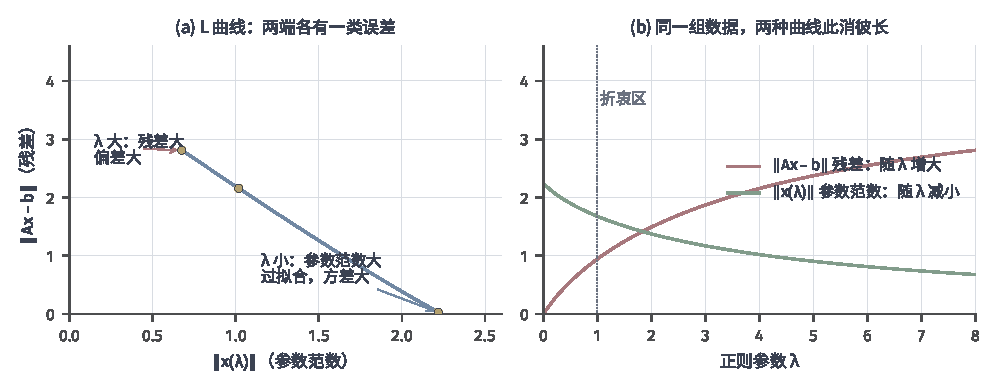
\includegraphics[width=168.998mm]{figures/01-mathematical-preliminaries-upper/02-linear-spaces/matplotlib/ls-regularization-bias-variance/ls-regularization-bias-variance.pdf}
  \caption{正则化的偏差—方差折中。$\bm A=\operatorname{diag}(2,1)$、$\bm b=(4,1)^\top$，
  岭解$\bm x(\lambda)=(8/(4+\lambda),1/(1+\lambda))^\top$。左：L曲线——横轴参数范数
  $\lVert\bm x(\lambda)\rVert$、纵轴残差$\lVert\bm A\bm x-\bm b\rVert$；右端（$\lambda$小）
  拟合准但参数大，左端（$\lambda$大）参数小但残差大。右：残差随$\lambda$上升、
  参数范数随$\lambda$下降，灰色虚线为折衷区。固定复算，无采样。}
  \label{fig:ls-regularization-bias-variance}
\end{figure*}

\section{二次优化}
\label{sec:ls-quadratic-optimization}

最小二乘目标本身是二次的；把“平方长度”推广到一般对称二次型，加上无约束、球面约束、
子空间约束与线性等式约束，得到一族可完全用代数配方和~\ref{sec:ls-svd}建立的谱定理
解决的优化问题。本节不使用微积分：所有最优性条件都由平方增量非负和正交关系得到。

\subsection{目标与约束}
\label{sec:ls-quadratic-goal}

一般二次目标写成（\term{二次型}，quadratic form）
\begin{equation}
 f(\bm x)=\frac12\bm x^\top\bm M\bm x+\bm c^\top\bm x,
 \label{eq:ls-general-quadratic}
\end{equation}
其中$\bm M$不必对称。反对称部分$\frac12(\bm M-\bm M^\top)$满足
$\bm x^\top(\bm M-\bm M^\top)\bm x=0$，故二次型只由对称部分
$\bm S=\frac12(\bm M+\bm M^\top)$决定，以下一律取$\bm S=\bm S^\top$。

无约束问题为$\min_{\bm x\in\mathbb R^d}f(\bm x)$；带线性等式约束为
\begin{equation}
 \min\ f(\bm x)\quad\text{s.t.}\quad \bm C\bm x=\bm d,
 \label{eq:ls-equality-constrained}
\end{equation}
$\bm C\in\mathbb R^{p\times d}$。可行性先于优化：$\bm C\bm x=\bm d$必须相容。

不含线性项时目标为$\bm x^\top\bm S\bm x$（可取$1/2$因子）。齐次性使目标在尺度缩放
下按平方变化，因而自然约束在单位球面$\lVert\bm x\rVert_2=1$、闭球
$\lVert\bm x\rVert_2\leq1$或某个子空间中；球面消除尺度自由度，只比较方向。

长度由$\bm B\succ0$度量时，约束为$\bm x^\top\bm B\bm x=1$，即\term{广义球面}；
它把加权长度固定，仍只优化方向。

\subsection{存在性与唯一性}
\label{sec:ls-quadratic-existence}

先判定目标在给定集合上是否有下界、极小点是否存在、是否唯一，再谈求解。

\subsubsection{无约束问题}
\label{sec:ls-unconstrained-existence}

先看三个二元例子区分目标形状：$f_1(x,y)=x^2+2y^2$恒正、原点是唯一谷底；
$f_2(x,y)=x^2$沿$y$轴整条等高，$f_2=0$取遍$(0,y)$，最小值集合是一条直线；
$f_3(x,y)=x^2-y^2$在原点一方向上谷、另一方向上脊，是鞍点。
图~\ref{fig:ls-quadratic-level-sets}把三类水平集并置：正定是同心椭圆，半正定退化为
平行直线槽，不定是双曲线。它们的差别只在$\bm S$的惯性（正、负、零特征值个数）。

\begin{figure*}[htbp]
  \centering
  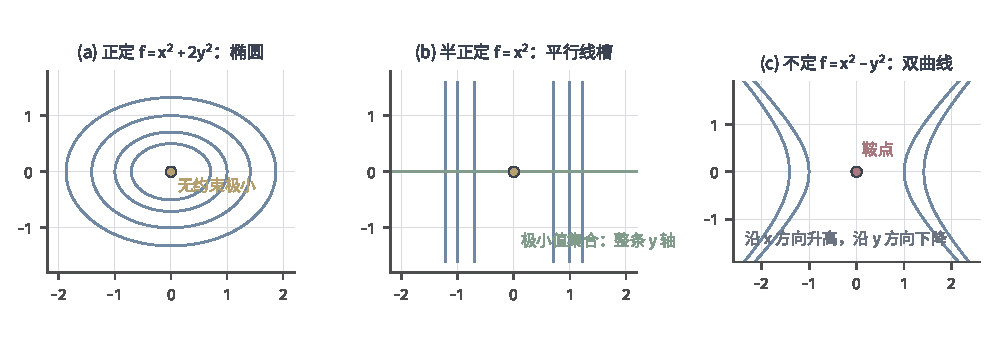
\includegraphics[width=168.998mm]{figures/01-mathematical-preliminaries-upper/02-linear-spaces/matplotlib/ls-quadratic-level-sets/ls-quadratic-level-sets.pdf}
  \caption{二次型水平集的三种情形。(a)正定$f=x^2+2y^2$：四层同心椭圆，黄点为唯一极小
  $(0,0)$；(b)半正定$f=x^2$：水平集退化为竖直线，绿线是极小值集合——整条$y$轴；
  (c)不定$f=x^2-y^2$：双曲线，红点为鞍点，沿$x$方向是谷、沿$y$方向是脊。
  解析式直接求值。}
  \label{fig:ls-quadratic-level-sets}
\end{figure*}

由谱引理~\ref{thm:ls-real-symmetric-spectral}，$\bm S$的正交谱展开把任意
$\bm x=\sum_i c_i\bm q_i$代入得
$f(\bm x)=\frac12\sum_i\lambda_i c_i^2+\sum_i c_i\bm c^\top\bm q_i$，每个方向独立。

若$\bm S$有负特征值$\lambda_j<0$，沿$\bm q_j$取$\bm x=t\bm q_j$，二次项
$\frac12\lambda_jt^2$按$t^2$趋向$-\infty$，线性项只按$t$一次增长，$|t|$足够大时
$t^2$项主导，目标无下界，不存在最小值。因此不定矩阵上的驻点不能当作最小点。

$\bm S\succeq0$时每个$\lambda_i\geq0$，二次项非负且沿正特征方向增长。零特征方向
$\lambda_j=0$上二次项为常数，目标只保留该方向的线性项；这些方向是否把目标拉向$-\infty$，
必须单独检查，不能因为二次项非负就认定有下界。

零方向$\bm q_j$上若有线性分量$\bm c^\top\bm q_j\neq0$，取$\bm x=t\bm q_j$，目标中的
线性项$t\,\bm c^\top\bm q_j$在$t\to-\infty$时趋向$-\infty$。故有下界的必要条件是
$\bm c\perp\ker\bm S$，由对称算子$\operatorname{range}\bm S=(\ker\bm S)^\perp$，
即$\bm c\in\operatorname{range}\bm S$。这也是正规方程$\bm S\bm x=-\bm c$相容的条件。

$\bm S\succ0$时所有$\lambda_i>0$，目标沿每个方向严格增长，唯一极小点。
$\bm S\succeq0$且$\bm c\in\operatorname{range}\bm S$时，正规方程相容，极小点存在
但沿$\ker\bm S$方向平坦，解集为仿射空间$\bm x_*+\ker\bm S$；不另加范数最小准则则
答案不唯一。

满足$\bm S\bm x+\bm c=0$的点只是驻点（最优性方程成立）。$\bm S$不定时，沿正特征方向
移动目标上升、沿负特征方向下降，驻点两侧一升一降，是鞍点而非最小点。不能把“方程成立”
当作“最小”，必须同时检查$\bm S$没有负方向；驻点条件只给出候选，不给出优劣判定。

\paragraph{惯性、合同判据与有界性}

$\bm S$的\term{惯性}（inertia）指正、负、零特征值的个数三元组$(n_+,n_-,n_0)$，由
谱引理唯一确定。目标有无下界恰由$n_-$判定：$n_->0$即存在负方向，目标无下界；
$n_-=0$（半正定）时二次项非负，目标有下界。合同变换（用可逆$\bm P$作
$\bm P^\top\bm S\bm P$）保持三个计数不变，故无需真的算出特征值，也可由对称消元记录
主元符号判断有界性。

\subsubsection{球面与子空间约束}
\label{sec:ls-sphere-existence}
\label{sec:linear-algebra-homogeneous-estimation}
\label{sec:linear-algebra-constrained-estimation}

单位球面$\{\bm x:\lVert\bm x\rVert_2=1\}$在有限维中是闭有界集，连续函数
$\bm x^\top\bm S\bm x$由~\ref{thm:ls-extreme-value}在球上同时取到最大值和最小值，
与$\bm S$是否正定无关；不定矩阵的两个极值分居零两侧。这一存在性不依赖方向是否可解，
先保证极值点存在，再讨论它落在哪个谱方向。

\paragraph{尺度消去与Rayleigh商}

齐次目标$\bm x^\top\bm S\bm x$在$\bm x\neq0$上按平方缩放变化，直接优化会被长度主导。
把长度约掉，方向评价写成\term{Rayleigh商}（Rayleigh quotient）
\begin{definition}[Rayleigh商]
\label{def:matrix-analysis-rayleigh-quotient}
\begin{equation}
 R_{\bm S}(\bm x)=\frac{\bm x^\top\bm S\bm x}{\bm x^\top\bm x},
 \label{eq:matrix-analysis-rayleigh-quotient}
\end{equation}
\end{definition}
它在$\bm x$缩放任意非零倍时不变，因此求$R_{\bm S}$的极值等价于在单位球面上求
$\bm x^\top\bm S\bm x$的极值，长度自由度被完全消去。

把$\bm x=\sum_i c_i\bm q_i$代入，分母$\sum_i c_i^2=1$（球面），
$R_{\bm S}(\bm x)=\sum_i\lambda_i c_i^2$是特征值以权重$c_i^2$（和为$1$）作的加权平均，
故落在$[\lambda_{\min},\lambda_{\max}]$内；令权重全给$\lambda_1$得最大值、全给
$\lambda_d$得最小值，且分别在$\bm q_1$、$\bm q_d$上取等。

$\lambda_i=\lambda_j$时，这两个特征向量的任意标准正交组合仍是该特征值的特征方向，
张成的子空间中每个单位向量都给出同一个极值商。故极值值唯一，达到它的方向一般不唯一；
仅当目标特征值单重时，方向才只差一个符号。图~\ref{fig:ls-sphere-constrained-extremum}
用一个二元对称矩阵把这一相切关系画出：极值椭圆恰在特征方向处与单位圆相切。

\begin{figure}[htbp]
  \centering
  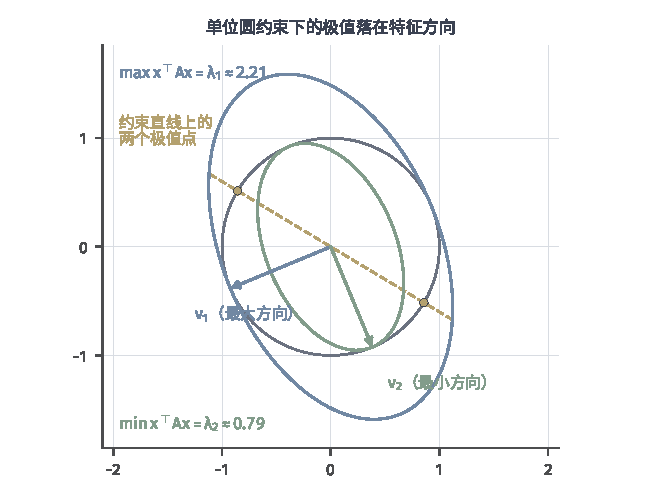
\includegraphics[width=112mm]{figures/01-mathematical-preliminaries-upper/02-linear-spaces/matplotlib/ls-sphere-constrained-extremum/ls-sphere-constrained-extremum.pdf}
  \caption{单位圆约束下的极值落在特征方向。$\bm S=\left[\begin{smallmatrix}2&0.5\\0.5&1\end{smallmatrix}\right]$，
  灰圆为$\lVert\bm x\rVert=1$。蓝椭圆$\bm x^\top\bm S\bm x=\lambda_1\approx2.21$在
  $\pm\bm v_1$处与单位圆相切（最大值），绿椭圆$=\lambda_2\approx0.79$在$\pm\bm v_2$处
  相切（最小值）；黄色虚线为子空间约束直线，其上黄点是该约束下的两个极值。
  $\lambda_{1,2}=(3\pm\sqrt2)/2$。固定复算。}
  \label{fig:ls-sphere-constrained-extremum}
\end{figure}

闭球$\lVert\bm x\rVert\leq1$是有界闭集，极值同样存在。$\bm S\succeq0$时最小值$0$
在内部$\bm x=0$取到，方向问题因此被迫放到边界；$\bm S$不定时最小值为负，落在
边界球面上，内部只含$\bm x=0$这个平凡点。所以“非零方向估计”必须主动固定单位长度，
否则齐次目标会把平凡解$\bm x=0$当作答案。

\paragraph{子空间约束下的同一问题}

限制在子空间$\mathcal W$中，问题仍是$\min_{\bm x\in\mathcal W}R_{\bm S}(\bm x)$，
由$\mathcal W$上的限制谱决定，是特征值交错与广义特征问题的入口。典型应用是
\term{齐次最小二乘}（homogeneous least squares）：模型写成$\bm A\bm h\approx\bm0$，
直接最小化$\lVert\bm A\bm h\rVert_2^2$总会接受平凡解$\bm h=\bm0$，必须先固定非零尺度：
\begin{equation}
 \min_{\lVert\bm h\rVert_2=1}\ \lVert\bm A\bm h\rVert_2^2
 =\min_{\lVert\bm h\rVert_2=1}\bm h^\top\bm A^\top\bm A\bm h.
 \label{eq:linear-algebra-homogeneous-least-squares}
\end{equation}
由Rayleigh--Ritz，最小值为$\bm A^\top\bm A$的最小特征值，最优$\bm h$是对应单位特征向量，
即最弱右奇异方向。$\bm A$有非零零空间时最小值为零，任一单位零空间向量都达到最优；
特别地$m<d$时不能只看紧致SVD列出的正奇异值而漏掉右零空间。最小特征值单重时方向只差
符号，重数更大则比例也不足以唯一确定。例如$\bm A=[\,1\ -2\,]$只要求$h_1=2h_2$，
单位解为$\pm(2,1)^\top/\sqrt5$，两个符号表示同一个实比例。

\subsubsection{线性等式约束}
\label{sec:ls-equality-existence}

优化只在可行集上进行，先判定$\bm C\bm x=\bm d$相容（$\bm d\in\operatorname{range}\bm C$）；
不相容时没有可行点，问题无解，谈不上优化。相容但$\bm C$的行线性相关时，多余方程是
独立方程的线性组合，不改变可行集，求解前可先去冗余，缩小约束规模。

取一个特解$\bm x_0$满足$\bm C\bm x_0=\bm d$，令$\mathcal N=\ker\bm C$，其标准正交基
排成矩阵$\bm N$。于是$\bm C(\bm x-\bm x_0)=\bm0$当且仅当$\bm x-\bm x_0\in\mathcal N$，
全部可行点参数化为$\bm x=\bm x_0+\bm N\bm z$，$\bm z$自由；可行方向就是$\mathcal N$。

把参数化代入$f(\bm x)=\frac12\bm x^\top\bm S\bm x+\bm c^\top\bm x$，二次项化为
$\bm z^\top(\bm N^\top\bm S\bm N)\bm z$，一次项化为
$\bm z^\top\bm N^\top(\bm c+\bm S\bm x_0)$，常数项与$\bm z$无关；问题化为
$\bm N^\top\bm S\bm N$在$\bm z$上的无约束二次问题，只在可行方向内检查曲率。

$\bm N^\top\bm S\bm N$在$\mathcal N$上正定，即$\bm z\neq0$时
$\bm z^\top\bm N^\top\bm S\bm N\bm z>0$；此时约化目标严格凸，唯一可行极小点，
代回参数化即得唯一$\hat{\bm x}$。

$\bm N^\top\bm S\bm N\succeq0$时，约化线性项$\bm N^\top(\bm c+\bm S\bm x_0)$
必须落在其值域内；若它沿某个零方向有分量，沿该方向移动时二次项不变而线性项下降，
目标无下界。条件满足时解集为$\bm x_*+\ker(\bm N^\top\bm S\bm N)$的仿射空间。

约化二次型在$\mathcal N$上有负方向，则沿该方向取$\bm x=\bm x_0+t\bm N\bm z$，
二次项按$t^2$趋向$-\infty$，约束问题无下界，与无约束情形同理。

\subsection{直接求解}
\label{sec:ls-quadratic-direct}

\subsubsection{无约束二次最小化}
\label{sec:ls-unconstrained-solve}

$\bm S\succ0$时把二次项配成完全平方：取$\bm x_*$满足$\bm S\bm x_*=-\bm c$，则
\[
 f(\bm x)-f(\bm x_*)=\frac12(\bm x-\bm x_*)^\top\bm S(\bm x-\bm x_*),
\]
右端因$\bm S$正定而非负，且只在$\bm x=\bm x_*$时为零。故$\bm S\bm x_*=-\bm c$给出
唯一最优线性方程，最小化问题归结为解这个正定对称方程。

$\bm S$正定，复用~\ref{sec:ls-direct-methods}的Cholesky分解$\bm S=\bm L\bm L^\top$，
先前代解$\bm L\bm y=-\bm c$，再回代解$\bm L^\top\bm x_*=\bm y$，避免形成逆矩阵。
分解与右端多重时可共享；这一路线与最小二乘正规方程用的是同一条正定对称求解流程。

$\bm S\succeq0$且$\bm c\in\operatorname{range}\bm S$时，$\bm S\bm x_*=-\bm c$相容。
由配方，任一解$\bm x_*$都是极小点；沿$\ker\bm S$移动二次项不变，全部解为
$\bm x_*+\ker\bm S$的仿射空间。不另加范数最小准则则答案不唯一，选代表的方法与普通
最小二乘的零空间选择相同。

核验两点：最优性方程$\bm S\hat{\bm x}+\bm c=0$成立；且对任意$\bm x$，增量
$\frac12(\bm x-\hat{\bm x})^\top\bm S(\bm x-\hat{\bm x})\geq0$非负。若增量沿某方向
为负，则该点不是最小点；方程成立只说明候选，符号检查才给出最小性。

\subsubsection{球面与子空间极值}
\label{sec:ls-sphere-solve}

\begin{theorem}[Rayleigh--Ritz]
\label{thm:matrix-analysis-rayleigh-ritz}
\label{eq:matrix-analysis-rayleigh-ritz}
设$\bm S$谱分解$\bm S=\sum_i\lambda_i\bm q_i\bm q_i^\top$，
$\lambda_1\geq\cdots\geq\lambda_d$，则
\begin{equation}
 \max_{\bm x\neq0}R_{\bm S}(\bm x)=\lambda_1\ \text{（在}\bm q_1\text{取到）},\qquad
 \min_{\bm x\neq0}R_{\bm S}(\bm x)=\lambda_d\ \text{（在}\bm q_d\text{取到）}.
\end{equation}
\end{theorem}
\begin{proof}
由谱展开$R_{\bm S}(\bm x)$是特征值的加权平均，故介于$\lambda_d$与$\lambda_1$之间；
取$\bm x=\bm q_1$、$\bm x=\bm q_d$时分别等于$\lambda_1$、$\lambda_d$，夹逼得端点取等。
\end{proof}

单方向极值只给$\lambda_1$与$\lambda_d$。要刻画中间的$\lambda_k$，取任意$k$维子空间
$\mathcal V$：它与$\operatorname{span}\{\bm q_k,\dots,\bm q_d\}$（维数$d-k+1$）的
维数之和$k+(d-k+1)=d+1>d$，故必有非零交点，交点处的Rayleigh商不大于$\lambda_k$。
换一个$d-k+1$维子空间与$\operatorname{span}\{\bm q_1,\dots,\bm q_k\}$同理相交。
这一维数交点关系是Courant--Fischer最小最大原理的几何来源。

\paragraph{Courant--Fischer的上下界与取等}

\begin{theorem}[Courant--Fischer]
\label{thm:matrix-analysis-courant-fischer}
\label{eq:matrix-analysis-courant-fischer}
\begin{equation}
 \lambda_k=\max_{\dim\mathcal V=k}\ \min_{\bm x\in\mathcal V,\bm x\neq0}R_{\bm S}(\bm x)
 =\min_{\dim\mathcal W=d-k+1}\ \max_{\bm x\in\mathcal W,\bm x\neq0}R_{\bm S}(\bm x).
\end{equation}
\end{theorem}
\begin{proof}
取$\mathcal V=\operatorname{span}\{\bm q_1,\dots,\bm q_k\}$，其中任意单位向量的
Rayleigh商不小于$\lambda_k$，给出下界；任一$k$维子空间与$\operatorname{span}\{\bm q_k,\dots,\bm q_d\}$
相交，交点处商不大于$\lambda_k$，给出上界。另一式由正交补同理得到。
\end{proof}
它不要求预先知道特征向量，为只需要第$k$个极值的子空间搜索提供了存在性表述。

\paragraph{正交列约束下的迹极值}

给定$k$个标准正交列$\bm V\in\mathbb R^{d\times k}$（$\bm V^\top\bm V=\bm I_k$），
\begin{theorem}[迹极值]
\label{thm:matrix-analysis-trace-minimum}
\label{eq:matrix-analysis-trace-minimum}
\begin{equation}
 \min_{\bm V^\top\bm V=\bm I_k}\operatorname{tr}(\bm V^\top\bm S\bm V)
 =\sum_{i=d-k+1}^d\lambda_i,
 \qquad
 \max_{\bm V^\top\bm V=\bm I_k}\operatorname{tr}(\bm V^\top\bm S\bm V)
 =\sum_{i=1}^k\lambda_i,
\end{equation}
\end{theorem}
\begin{proof}
由谱展开$\operatorname{tr}(\bm V^\top\bm S\bm V)=\sum_i\lambda_i\lVert\bm q_i^\top\bm V\rVert_2^2$，
权重$\lVert\bm q_i^\top\bm V\rVert_2^2$非负且总和为$k$；把权重配给最小的$k$个
$\lambda_i$得最小值，配给最大的$k$个得最大值，对应特征向量张成达到取等。
\end{proof}
最小值由$k$个最小特征向量张成，最大值由$k$个最大特征向量张成；这是后续正交拟合与
低秩方向提取的代数基础。

广义约束$\bm x^\top\bm B\bm x=1$、$\bm B\succ0$，先由Cholesky
$\bm B=\bm R^\top\bm R$令$\bm z=\bm R\bm x$，则约束化为$\lVert\bm z\rVert_2=1$，
目标$\bm x^\top\bm S\bm x$化为$\bm z^\top\bm R^{-\top}\bm S\bm R^{-1}\bm z$，成为
普通对称矩阵$\bm R^{-\top}\bm S\bm R^{-1}$的Rayleigh商，可直接用单方向极值结论。

\paragraph{广义特征问题与方向恢复}

\begin{definition}[广义特征值]
\label{def:matrix-analysis-generalized-eigenvalue}
白化后的对称问题等价于\term{广义特征问题}
\begin{equation}
 \bm S\bm v=\mu\bm B\bm v,
 \label{eq:matrix-analysis-generalized-eigenproblem}
\end{equation}
\end{definition}
白化后普通特征向量$\bm z$恢复原方向$\bm v=\bm R^{-1}\bm z$；广义极值即$\mu$的最大、
最小值，方向按此恢复。不要直接对$\bm B^{-1}\bm S$（一般非对称）求特征，其特征值可能为
复数而失去极值意义。

\subsubsection{等式约束二次最小化}
\label{sec:ls-equality-solve}

由可行点参数化$\bm x=\bm x_0+\bm N\bm z$，把约束消去后，目标化为$\bm z$上的无约束
二次问题，正规方程为
$(\bm N^\top\bm S\bm N)\bm z=-\bm N^\top(\bm c+\bm S\bm x_0)$；解出$\bm z$后按
$\bm x=\bm x_0+\bm N\bm z$拼回原变量。这一路线先把可行性编入参数化，求解时不必再
显式处理约束。

约化矩阵$\bm N^\top\bm S\bm N$正定即按无约束流程Cholesky求解，得到唯一$\hat{\bm z}$；
半正定则按值域条件解相容方程，在全部最小点中选代表。约化矩阵维数等于$\ker\bm C$的
维数，通常小于原问题规模。

对任意可行方向$\bm\delta$（$\bm C\bm\delta=0$），目标沿$\bm\delta$的一阶变化为
$\bm\delta^\top(\bm S\bm x+\bm c)$，最优性要求它为零。这说明$\bm S\bm x+\bm c$正交于
$\ker\bm C$，由正交补关系落在$\operatorname{range}(\bm C^\top)$，故存在乘子$\bm\mu$
使$\bm S\bm x+\bm c=\bm C^\top\bm\mu$；$\bm\mu$衡量约束方向上的平衡量。

\paragraph{KKT系统的分块构造}

联立约束$\bm C\bm x=\bm d$与最优性$\bm S\bm x+\bm c=\bm C^\top\bm\mu$，得到
\term{KKT条件}（KKT conditions）分块系统
\begin{equation}
 \begin{bmatrix}\bm S&\bm C^\top\\ \bm C&\bm0\end{bmatrix}
 \begin{bmatrix}\bm x\\ \bm\mu\end{bmatrix}
 =\begin{bmatrix}-\bm c\\ \bm d\end{bmatrix}.
 \label{eq:ls-kkt-system}
\end{equation}
它同时编码可行性（第二块行）与最优性（第一块行），由正交关系推出，不需要微分记号。

对分块系统可先消元（把$\bm\mu$从第一行解出代回），或对分块矩阵作适当分解直接求解，
同时得到$\bm x$与$\bm\mu$。$\bm\mu$只是伴随约束的对偶量，不改变原目标值，核验时
主要保证$\bm x$满足原目标与约束。

$\ker\bm C\cap\ker\bm S=\{\bm0\}$时$\bm\mu$唯一；约束冗余（$\bm C$行相关）时
$\operatorname{range}\bm C^\top$维数小于行数，$\bm\mu$可加$\ker\bm C^\top$中的量而
不改变方程，乘子不唯一，但可行方向正定时原变量$\bm x$仍可唯一。

分别核验：可行性$\bm C\hat{\bm x}=\bm d$；最优性$\bm S\hat{\bm x}+\bm c\in\operatorname{range}(\bm C^\top)$，
即对所有$\bm\delta\in\ker\bm C$有$\bm\delta^\top(\bm S\hat{\bm x}+\bm c)=0$。只满足约束
或只满足方程都不是合格最小点，二者缺一不可。

\subsection{迭代求解}
\label{sec:ls-quadratic-iterative}

直接法需要分解矩阵；只给矩阵作用时用迭代逼近谱方向或正定极小点，收敛速度证明留待
迭代收敛章节。

$\bm S\succ0$的无约束问题$\bm S\bm x=-\bm c$本身就是正定对称线性方程，直接复用
~\ref{sec:ls-krylov-methods}的共轭梯度法：每步只调用$\bm S$对向量的乘积，不形成分解，
更新格式、有限步终止与停止核验在该处建立，此处不重述。

求最大特征方向时反复$\bm v\leftarrow\bm S\bm v/\lVert\bm S\bm v\rVert_2$：每次作用把
最大特征值方向按$\lambda_1$放大，其余方向按比值$\lambda_i/\lambda_1$相对缩小，归一化
后方向逐次偏向$\bm q_1$。相邻特征值分离越快，比值越小，方向提取越直接；分离程度决定
收敛快慢，定量速率留待迭代收敛章节。

求靠近$\rho$的特征方向时迭代$(\bm S-\rho\bm I)^{-1}\bm v$，要求$\bm S-\rho\bm I$可逆
（$\rho$不是特征值）。移位后靠近$\rho$的特征值变为大数，其分量被逐步放大；每步解一个
移位线性系统而非求逆矩阵，收敛速度由目标与邻近特征值的距离决定。

Lanczos用短递推把$\bm S$投影成三对角小矩阵，在小矩阵上求极值方向再经基映回原空间；
只调用乘积、存储随步数线性增长，适合只需要少数几个极值方向、矩阵不能整体分解的情形。
有限步理论与收敛速率属迭代收敛章节。

\section{矩阵低秩逼近}
\label{sec:ls-matrix-low-rank}
\label{sec:matrix-analysis-svd-low-rank}
\label{sec:ch06-rank-constrained-approximation}
\label{sec:ch06-error-constrained-rank}

第~\ref{sec:ls-least-squares}节在固定形状的输入向量中挑选系数，使输出残差最小；
本节改变任务对象：未知量本身是一张矩阵，要求它在保持主要作用的同时占用更少参数。
一张$m\times n$稠密矩阵需要存储$mn$个数，每次作用需要$O(mn)$次运算；推荐系统的评分
矩阵、一幅图像或一批样本的设计矩阵，$mn$轻易达到百万级，直接存储和运算都不现实。
这类矩阵的信息常高度集中：少数几个输入方向被放大后送入配对的输出方向，就解释了大部分
作用。自然的问题是：能否只保留最重要的$k$个方向，用远少于$mn$的参数近似整张矩阵？
若能以$k$个输入输出方向的配对近似它，存储和作用成本便可降到$O((m+n)k)$。

特征向量要求输出回到输入的同一方向，因而适合分析同一空间内的反复作用；压缩却要问哪些
输入方向的作用最值得保留，并允许输出落到另一个方向。三维输入送入二维输出时已经无法要求
两端沿同一条方向；又如把用户作为行、影片作为列，评分矩阵$\bm R\in\mathbb R^{n_{\mathrm u}\times n_{\mathrm m}}$
中$\bm v\mapsto\bm R\bm v$把影片坐标映到用户坐标，两端本就是不同对象的坐标，谈不上同一个
特征方向。因此本节使用第~\ref{sec:ls-svd}节已经建立的奇异值分解：定义域与陪域各自选取
正交方向，有非零作用的输入方向分别被缩放后送入配对的输出方向，其余方向映为零。
存在性与构造不再重复，本节只在这一工具上回答规模怎样度量、最优候选是谁、怎样计算与核验。

\subsection{目标与误差}
\label{sec:ls-low-rank-objective}

\paragraph{秩预算与误差范数}

先规定规模预算：给定整数$k$，在所有秩不超过$k$的矩阵中寻找离$\bm A$最近的候选
$\bm B$。误差口径先于方向选择确定，常用两种：谱范数误差
$\lVert\bm A-\bm B\rVert_2=\max_{\lVert\bm x\rVert_2=1}\lVert(\bm A-\bm B)\bm x\rVert_2$
度量任意单位输入的最坏输出偏差；Frobenius误差
$\lVert\bm A-\bm B\rVert_{\mathrm F}=(\sum_{i,j}(a_{i,j}-b_{i,j})^2)^{1/2}$
对一组标准输入方向的输出偏差平方求和后开方。两者回答不同问题：前者保证最坏方向不失真，
后者累计全部坐标的总偏差，不能互相替代。

由~\ref{thm:ls-svd-existence}，$\bm A\in\mathbb R^{m\times n}$有分解
$\bm A=\bm U\bm\Sigma\bm V^\top$，非零奇异值按降序记为
$\sigma_1\geq\cdots\geq\sigma_r>0$，$r=\operatorname{rank}\bm A$。
下面所有结论都以这一给定分解为输入，不再重新证明奇异值的存在性。

\paragraph{秩约束与核范数惩罚的区别}

固定秩约束$\operatorname{rank}\bm B\leq k$是一个硬预算：可行集合由若干低维线性流形
拼成，不是凸集，候选不能沿线段自由插值。另一条路线不在参数上设限，而在拟合目标中附加
对矩阵“大小”的凸惩罚：
\begin{equation}
 \min_{\bm B}\ \tfrac12\lVert\bm A-\bm B\rVert_{\mathrm F}^2
 +\lambda\lVert\bm B\rVert_*,
 \qquad \lambda\geq0,
 \label{eq:ls-nuclear-penalty-problem}
\end{equation}
其中$\lVert\cdot\rVert_*$是稍后定义的核范数。惩罚改变的是目标本身：$\lambda$越大，
保留下来的奇异尺度被压得越小，它产生的实际秩取决于原谱，不等于直接指定$k$。
硬预算回答“最多用$k$个方向能做到多好”，惩罚问题回答“拟合与简洁之间怎样折中”，
两者的最优解一般不同，求解路径也不同，不能不加说明地当成同一个截断问题。

\subsection{规模与误差的比较}
\label{sec:ls-rank-scale-comparison}

\subsubsection{秩与保留信息}
\label{sec:ls-rank-and-information}

\paragraph{精确非零方向与代数秩}

代数秩$r=\operatorname{rank}\bm A$是非零奇异值的个数，也就是$\bm A$真正使用的
精确非零方向数：$\bm A=\sum_{i=1}^r\sigma_i\bm u_i\bm v_i^\top$中每一项对应一对
独立的伸缩方向，$\sigma_i=0$的方向不参与作用。代数秩是离散整数，对任意小的秩增加
扰动都可能跳变：$\operatorname{diag}(1,\varepsilon)$的代数秩恒为$2$，尽管
$\varepsilon\to0$时第二个方向的作用趋于消失。因此它描述“精确表示需要几项”，
不直接回答“近似表示保留几项足够”。

\paragraph{容差与数值秩}

数据带有噪声时，把低于某一绝对阈值$\tau$的奇异值视为零更符合实际。\term{数值秩}
（numerical rank）定义为
\begin{equation}
 r_{\mathrm{num}}(\bm A;\tau)=\#\{i:\sigma_i>\tau\}.
 \label{eq:ls-numerical-rank}
\end{equation}
它恰好等于谱范数误差不超过$\tau$时所需的最小秩（见~\ref{sec:ls-low-rank-solve}），
但必须同时说明阈值口径：绝对阈值$\tau$与相对阈值$\tau=\epsilon\lVert\bm A\rVert_2$
给出不同计数，零矩阵不能计算$0/0$。数值秩不是一个不含容差的固定数值，换一个阈值
就换一个数。

\paragraph{谱能量分布与稳定秩}

代数秩和数值秩都是整数计数，能量集中程度则需要一个连续尺度。非零矩阵$\bm A$的
\term{稳定秩}（stable rank）\label{def:matrix-analysis-stable-rank}定义为
\begin{equation}
 r_{\mathrm{stable}}(\bm A)
 =\frac{\lVert\bm A\rVert_{\mathrm F}^2}{\lVert\bm A\rVert_2^2}
 =\frac{\sum_{i=1}^r\sigma_i^2}{\sigma_1^2},
 \label{eq:matrix-analysis-stable-rank}
\end{equation}
零矩阵另约定为零。由$\sigma_1^2\leq\sum_i\sigma_i^2\leq r\sigma_1^2$，
$1\leq r_{\mathrm{stable}}\leq r$：所有非零奇异值相等时取到$r$，能量几乎全在
首方向时接近$1$。例如奇异值$(8,3,1,0.2)$的稳定秩为
$74.04/64\approx1.157$，说明能量高度集中在第一个方向，尽管代数秩是$4$。

\paragraph{有效秩的不同归一化口径}

稳定秩是\term{有效秩}（effective rank）的一种，另一种常用口径把奇异值归一化为
概率分布$p_i=\sigma_i/\sum_j\sigma_j$，再取熵的指数
\begin{equation}
 r_{\mathrm{ent}}(\bm A)
 =\exp\!\left(-\sum_i p_i\log p_i\right),
 \qquad 0\log0=0.
 \label{eq:ls-effective-rank-entropy}
\end{equation}
也有版本用平方奇异值归一化$p_i=\sigma_i^2/\sum_j\sigma_j^2$，两种口径数值一般不同。
它们都是连续的能量分散度，不是误差阈值下的最优整数秩：上例的$1.157$既不是
$\tau=1$时的谱最优秩$2$，也不是Frobenius最优秩$3$。它也不同于后续正则化讨论中
随惩罚尺度变化的核有效维度，不要混用。

\paragraph{零矩阵与连续性边界}

稳定秩在非零矩阵处连续且不随整体缩放改变（分子分母同乘$c^2$），但零矩阵的约定值$0$
不使它在零处连续：$\operatorname{diag}(1,\varepsilon)$的稳定秩趋于$1$而不是$0$。
有效秩的各归一化口径有同样的边界行为。因此涉及零矩阵时必须单独处理，不能把连续尺度
公式直接代入；工程上先判$\bm A=\bm0$再计算任何比值。

\paragraph{规模指标与最小可行秩的区别}

代数秩、数值秩、稳定秩与有效秩回答不同问题：代数秩是精确表示的项数，数值秩是阈值下的
计数，稳定秩和有效秩是能量分散的连续描述；而“给定误差预算至少要保留几项”是
~\ref{sec:ls-low-rank-solve}要解的优化问题的答案。规模指标不能代替误差预算，
误差预算也不给出能量分散度。此外，谱范数次乘
$\lVert\bm A_L\cdots\bm A_1\rVert_2\leq\prod_\ell\lVert\bm A_\ell\rVert_2$
不蕴含稳定秩可以逐层相乘：各层的最强方向未必对齐，上界可能宽松。

\subsubsection{误差与方向选择}
\label{sec:ls-direction-pairing}

\paragraph{固定奇异值下的方向选择}

求最佳低秩候选之前，先解决一个更一般的子问题：固定候选$\bm B$的奇异值$s_1\geq\cdots\geq0$，
只让它的左右奇异方向自由，怎样配对才能使$\bm B$离$\bm A$最近？这一子问题同时服务于
固定秩截断和核范数惩罚，结论被~\ref{sec:ls-orthogonal-approximation}节与
~\ref{sec:ls-symmetric-spectral-approximation}节复用。

\paragraph{迹展开与方向配对权重}

设$\bm A=\bm U\Sigma\bm V^\top$，$\bm B=\widehat{\bm U}\widehat\Sigma\widehat{\bm V}^{\,\top}$，
两端标准内积为Frobenius配对$\langle\bm X,\bm Y\rangle_{\mathrm F}
=\operatorname{tr}(\bm X^\top\bm Y)$（见~\ref{sec:ls-matrix-contractions}）。
展开平方距离的交叉项：
\begin{equation}
 \operatorname{tr}(\bm B^\top\bm A)
 =\sum_{i,j}s_i\sigma_j
   (\widehat{\bm u}_i^\top\bm u_j)(\widehat{\bm v}_i^\top\bm v_j).
 \label{eq:ls-trace-pairing-expand}
\end{equation}
令$c_{i,j}=|\widehat{\bm u}_i^\top\bm u_j|\,|\widehat{\bm v}_i^\top\bm v_j|$，
距离中的交叉项只通过这个配对权重依赖方向。

\paragraph{配对权重的行列和约束}

固定$i$，由Cauchy--Schwarz与正交投影不增加长度，
$\sum_j|\widehat{\bm u}_i^\top\bm u_j|^2\leq1$、
$\sum_j|\widehat{\bm v}_i^\top\bm v_j|^2\leq1$，故
\begin{equation}
 \sum_j c_{i,j}\leq1,\qquad
 \sum_i c_{i,j}\leq1.
 \label{eq:ls-pairing-weight-marginals}
\end{equation}
每行、每列的权重和都不超过$1$，总权重和不超过$\min(m,n)$。

\paragraph{有序奇异值的配对上界与取等}

把奇异值写成相邻差分的和，前$k$行、前$\ell$列的权重和$C_{k,\ell}\leq\min(k,\ell)$，
于是
\begin{equation}
 \sum_{i,j}\alpha_i\beta_j c_{i,j}
 \leq\sum_{i=1}^q\alpha_i\beta_i,
 \qquad
 \alpha_i=\sigma_i(\bm A),\ \beta_i=s_i(\bm B)
 \text{ 均降序排列}.
 \label{eq:ls-rearrangement-trace-bound}
\end{equation}
差分展开后$\min(k,\ell)=\sum_i\mathbf 1\{i\leq k,\ i\leq\ell\}$，两侧分别求差分和即得。
上界在$\bm B$与$\bm A$使用相同左右奇异方向时取等：$\widehat{\bm u}_i=\bm u_i$、
$\widehat{\bm v}_i=\bm v_i$。这就是有序奇异值的配对不等式：大配大、小配小不损失配对，
交叉配对只会减小$\operatorname{tr}(\bm B^\top\bm A)$。

\paragraph{Schatten范数的对偶表达}

由配对上界可以建立一族矩阵尺度。对$1\leq p<\infty$，\term{Schatten $p$范数}
（Schatten $p$-norm）定义为
\begin{equation}
 \lVert\bm A\rVert_{S_p}
 =\left(\sum_i\sigma_i^p\right)^{1/p},
 \qquad
 \lVert\bm A\rVert_{S_\infty}=\sigma_1,
 \label{def:matrix-analysis-schatten-norm}
\end{equation}
零矩阵的值为零。$p=1,2,\infty$依次给出核范数
$\lVert\bm A\rVert_*=\sum_i\sigma_i$\label{eq:matrix-analysis-nuclear-norm}、Frobenius范数
$\lVert\bm A\rVert_{\mathrm F}=(\sum_i\sigma_i^2)^{1/2}$\label{eq:matrix-analysis-frobenius-norm}与谱范数
$\lVert\bm A\rVert_2=\sigma_1$\label{eq:matrix-analysis-spectral-norm}；这三个谱表达式是~\ref{thm:ls-svd-existence}的直接推论，
不再重复推导。Schatten范数在两端正交换基下不变，只关心伸缩谱。

标量Hölder不等式给出对偶关系：对共轭指数$1/p+1/q=1$，
\begin{equation}
 \lVert\bm A\rVert_{S_p}
 =\max_{\lVert\bm B\rVert_{S_q}\leq1}
 |\operatorname{tr}(\bm B^\top\bm A)|.
 \label{eq:ls-schatten-duality}
\end{equation}
取达到构造：$1<p<\infty$时令$\bm B$与$\bm A$同方向、奇异值
$b_i=\sigma_i^{p-1}/\lVert\bm A\rVert_{S_p}^{p-1}$；$p=1$时在每个正奇异方向取
$b_i=1$；$p=\infty$时只在最大奇异方向取$b_i=1$。$\bm A=\bm0$时取$\bm B=\bm0$。
因此核范数是谱范数的对偶，Frobenius范数自对偶。

\paragraph{三角不等式与核范数合法性}

线性配对在单位球上的最大值自动满足三角不等式、齐次性与正定性，所以对偶是范数；
核范数作为谱范数的对偶，本身是合法范数，其单位球凸，~\eqref{eq:ls-nuclear-penalty-problem}
是凸优化问题。$0<p<1$沿用同一公式只得到拟范数：
$\bm A=\operatorname{diag}(1,0)$、$\bm B=\operatorname{diag}(0,1)$时
$\lVert\bm A+\bm B\rVert_{S_p}=2^{1/p}>2$，违反三角不等式，不能当作凸惩罚使用。

\paragraph{秩相关的范数比较}

对秩为$r$的矩阵，由$\sigma_1\leq(\sum_i\sigma_i^p)^{1/p}$等逐项比较得到
\begin{equation}
 \lVert\bm A\rVert_2\leq\lVert\bm A\rVert_{\mathrm F}
 \leq\sqrt r\,\lVert\bm A\rVert_2,\qquad
 \lVert\bm A\rVert_{\mathrm F}\leq\lVert\bm A\rVert_*
 \leq\sqrt r\,\lVert\bm A\rVert_{\mathrm F}.
 \label{eq:matrix-analysis-norm-rank-relations}
\end{equation}
常数带秩因子，范数等价在这里不是无代价的。多个方向同时被舍弃时，最坏方向误差
（谱口径）和总平方误差（Frobenius口径）不能用同一个舍弃奇异值代替。
\subsection{存在性与唯一性}
\label{sec:ls-low-rank-existence}

\paragraph{最佳低秩近似的存在性}

固定$k$，可行集合$\{\bm B:\operatorname{rank}\bm B\leq k\}$是所有$(k+1)$阶子式
同时为零的集合，因而是闭集。取使$\lVert\bm A-\bm B\rVert$收敛到下确界的极小化序列
$\bm B_t$，它必有界：否则由三角不等式
$\lVert\bm B_t\rVert\leq\lVert\bm A\rVert+\lVert\bm A-\bm B_t\rVert$，而误差序列
有界。有限维中闭有界集上的连续范数函数取到极值（~\ref{thm:ls-extreme-value}），
故极限$\bm B_*$仍在可行集合内并达到最小误差。谱范数与Frobenius范数下存在性相同，
区别只在最优解是否唯一。

\paragraph{奇异值间隙与Frobenius最优解的唯一性}

Frobenius目标下，当$1\leq k<r$且$\sigma_k>\sigma_{k+1}$有严格间隙时，最佳矩阵唯一：
严格间隙迫使最优保留子空间恰好由前$k$个右奇异向量张成，误差平方的对齐项又把投影结果
确定下来。边界奇异值相等时，对应重特征子空间内的任意标准正交旋转仍给出同一最优值，
最佳矩阵不唯一，但最佳值唯一。

\paragraph{谱范数误差下的非唯一性}

谱目标即使有严格间隙也未必唯一。例如$\bm A=\operatorname{diag}(2,0.4)$，
$\bm B_t=\operatorname{diag}(2+t,0)$对$|t|\leq0.4$都以谱误差$0.4$近似$\bm A$，
候选矩阵互不相同。因此谱口径下只能保证最佳值$\sigma_{k+1}$达到，不能宣称唯一候选；
需要唯一解时应改用Frobenius口径并检查间隙。

\subsection{秩约束的求解}
\label{sec:ls-low-rank-solve}

\subsubsection{基于完整分解的求解}
\label{sec:ls-full-svd-solve}

\paragraph{截断SVD候选的构造}

取前$k$个奇异方向构造候选\term{截断SVD}（truncated SVD）
\begin{equation}
 \bm A_k=\sum_{i=1}^k\sigma_i\bm u_i\bm v_i^\top,
 \qquad 0\leq k<r,
 \label{eq:matrix-analysis-truncated-svd}
\end{equation}
$k=0$为空和$\bm0$。它只保留最大的$k$个伸缩方向，尾部$\bm A-\bm A_k$由剩余奇异项
组成。

\paragraph{谱误差与Frobenius误差}

由分解形式直接读出两种误差：
\begin{equation}
 \lVert\bm A-\bm A_k\rVert_2=\sigma_{k+1},\qquad
 \lVert\bm A-\bm A_k\rVert_{\mathrm F}
 =\left(\sum_{i=k+1}^r\sigma_i^2\right)^{1/2}.
 \label{eq:ls-truncated-errors}
\end{equation}
谱误差是尾部最大奇异值，Frobenius误差是尾部能量开方；只舍弃一个方向时两者相等，
多个尾方向时必须分别取最大值与平方和。

\paragraph{任意低秩候选的误差下界}

截断候选为什么最优，需要对任意秩不超过$k$的$\bm B$证明误差不能更小。谱口径：
$S=\operatorname{span}\{\bm v_1,\ldots,\bm v_{k+1}\}$为$k+1$维，而
$\dim\ker\bm B\geq n-k$，二者必有非零交向量。取单位向量
$\bm x=\sum_{i=1}^{k+1}c_i\bm v_i\in S\cap\ker\bm B$，则
\begin{equation}
 \lVert(\bm A-\bm B)\bm x\rVert_2
 =\lVert\bm A\bm x\rVert_2
 =\left(\sum_{i=1}^{k+1}\sigma_i^2c_i^2\right)^{1/2}
 \geq\sigma_{k+1}.
 \label{eq:ls-spectral-lower-bound}
\end{equation}
Frobenius口径：令$\bm C=\bm U^\top\bm B\bm V$，其列空间正交投影为$\bm P$，按列
正交分解得
$\lVert\Sigma-\bm C\rVert_{\mathrm F}^2
=\lVert(\bm I-\bm P)\Sigma\rVert_{\mathrm F}^2
+\lVert\bm P\Sigma-\bm C\rVert_{\mathrm F}^2$。
第二项非负；第一项中保留能量
$\lVert\bm P\Sigma\rVert_{\mathrm F}^2
=\sum_i\sigma_i^2\lVert\bm P\bm e_i\rVert_2^2$，权重在$[0,1]$内且总和不超过
$\operatorname{tr}\bm P\leq k$，由~\ref{sec:ls-direction-pairing}的权重论证不超过
$\sum_{i=1}^k\sigma_i^2$，故误差平方至少为尾能量$\sum_{i>k}\sigma_i^2$。

\paragraph{最佳近似与取等条件}

\begin{theorem}[Eckart--Young--Mirsky最佳低秩逼近]
\label{thm:ls-best-low-rank}
\label{thm:matrix-analysis-best-low-rank}
对$0\leq k<r=\operatorname{rank}\bm A$，
\begin{align}
 \min_{\operatorname{rank}\bm B\leq k}\lVert\bm A-\bm B\rVert_2
 &=\sigma_{k+1},
 \label{eq:matrix-analysis-best-rank-k-spectral}\\
 \min_{\operatorname{rank}\bm B\leq k}\lVert\bm A-\bm B\rVert_{\mathrm F}
 &=\left(\sum_{i=k+1}^r\sigma_i^2\right)^{1/2}.
 \label{eq:matrix-analysis-best-rank-k-frobenius}
\end{align}
两个最小值均由截断候选$\bm A_k$达到；$k\geq r$时取$\bm A_k=\bm A$，最小误差为零。
\end{theorem}
\scite{eckart1936}
下界已由上段给出；$\bm A-\bm A_k$的最大奇异值恰为$\sigma_{k+1}$、其Frobenius范数
恰为尾能量开方，故下界同时达到。谱误差控制任意单位输入的最坏输出偏差，Frobenius误差
累计标准正交输入的总偏差；其他加权、逐元素或分组误差需要重新核对最优性，不能自动沿用
本定理。

\paragraph{由误差容限选择秩}

若系统规定输出误差不能超过$\tau$，应反过来求最小可行秩。记$\sigma_{r+1}=0$，两条
最优误差曲线为$e_2(k)=\sigma_{k+1}$、
$e_{\mathrm F}(k)=(\sum_{i>k}\sigma_i^2)^{1/2}$，$k=0,\ldots,r$。它们是所有该规模
候选的最低误差，不是启发式算法的误差，因此
\begin{equation}
 k_2(\tau)=\min\{k:\sigma_{k+1}\leq\tau\}=\#\{i:\sigma_i>\tau\},
 \label{eq:ch06-minimum-rank-under-error}
\end{equation}
$k_{\mathrm F}(\tau)=\min\{k:\sum_{i>k}\sigma_i^2\leq\tau^2\}$。
截断SVD在这两个最小整数上提供可行解，任何更小秩都被最优下界排除。阈值恰好等于某奇异值
时“不超过”允许舍弃该方向，故计数用严格大于。$\tau=0$需要代数秩；谱口径允许秩零的
条件是$\tau\geq\lVert\bm A\rVert_2$，Frobenius口径则要求$\tau\geq\lVert\bm A\rVert_{\mathrm F}$。
相对预算$\epsilon$分别令$\tau=\epsilon\lVert\bm A\rVert_2$或
$\tau=\epsilon\lVert\bm A\rVert_{\mathrm F}$，零矩阵直接处理。

例如奇异值$(8,3,1,0.2)$时，秩$0$至$4$的谱误差为$(8,3,1,0.2,0)$，Frobenius误差为
$(\sqrt{74.04},\sqrt{10.04},\sqrt{1.04},0.2,0)$。阈值$\tau=1$在谱口径下只需
$k=2$，在Frobenius口径下却需$k=3$，因为两个被舍弃方向合计平方误差$1.04>1$。
图~\ref{fig:ch06-error-rank-curves}用同一谱展示两种读取方式。

\begin{figure}[htbp]
  \centering
  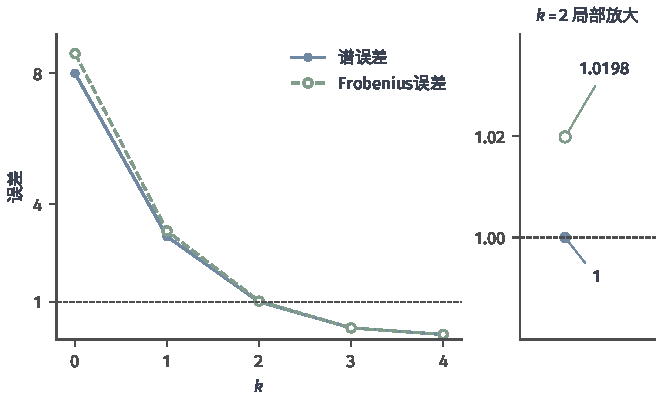
\includegraphics[width=112.0mm]{figures/01-mathematical-preliminaries-upper/02-linear-spaces/matplotlib/ch06-error-rank-curves/figure.pdf}
  \caption{固定奇异值$(8,3,1,0.2)$的最优误差曲线。给定横轴的秩可读出最低误差；
  给定水平误差阈值则寻找第一个满足要求的整数秩。$\tau=1$时，蓝色谱误差在
  $k=2$达标，绿色Frobenius误差要到$k=3$才达标。连线只辅助阅读，可行秩为整数。}
  \label{fig:ch06-error-rank-curves}
\end{figure}

\paragraph{中心化数据与PCA重构}

固定有限数据的重构是同一结论的实例。设$\bm X\in\mathbb R^{n\times d}$每行是一个样本，
先减去样本均值使每列之和为零。选择$\bm W^\top\bm W=\bm I_k$，低维坐标
$\bm Z=\bm X\bm W$，重构$\widehat{\bm X}=\bm Z\bm W^\top$，则
\begin{equation}
 \lVert\bm X-\bm X\bm W\bm W^\top\rVert_{\mathrm F}^2
 =\lVert\bm X\rVert_{\mathrm F}^2-\lVert\bm X\bm W\rVert_{\mathrm F}^2
 =\lVert\bm X\rVert_{\mathrm F}^2
 -\operatorname{tr}(\bm W^\top\bm X^\top\bm X\bm W).
 \label{eq:ls-pca-reconstruction}
\end{equation}
~\ref{sec:ls-quadratic-optimization}节的迹极值说明，最大化保留能量即取前$k$个右奇异
向量，重构恰为$\bm X_k$。这就是\term{主成分分析}（principal component analysis，PCA）
的有限矩阵形式；$n\geq2$时样本协方差$\bm X^\top\bm X/(n-1)$使保留方差总和为
$\lVert\bm X\bm W\rVert_{\mathrm F}^2/(n-1)$，最大化保留样本方差与最小化平方重构误差
等价。

例如四个中心化样本$(2,0)$、$(-2,0)$、$(0,1)$、$(0,-1)$，Gram矩阵为
$\operatorname{diag}(8,2)$。取$k=1$得$\bm W=(1,0)^\top$，坐标为$(2,-2,0,0)^\top$，
后两个样本都重构成零，误差平方为$2$。未中心化时，最强方向可能反映数据整体离原点的
位置而非围绕均值的变化；重构原始数据还应加回均值。把米改成毫米也会改变欧氏目标，是否
标准化必须由任务决定。最大样本方差不自动等于最有预测价值的方向，对总体协方差的估计
保证需要后续统计假设。

\paragraph{因子存储与作用代价}

以紧致因子存储$\bm A_k=\bm U_k\Sigma_k\bm V_k^\top$需要约$(m+n)k+k$个数，作用于一个
输入可先算$\bm V_k^\top\bm x$、按$\sigma_i$缩放、再乘$\bm U_k$。只有$k$相对两端
维数足够小时才真正节省存储和计算；小矩阵中因子开销可能更大。求SVD本身也有成本，不能
只统计后续乘法。噪声尺度若高于最后保留的奇异值，把$k$算得很精确也不等于方向可辨认，
方向可靠性由后续扰动分析章的谱隙条件判断。

\subsubsection{基于子空间压缩的近似求解}
\label{sec:ls-subspace-compression}

\paragraph{近似列空间与正交基}

完整SVD对超大矩阵代价过高。另一条路线把大矩阵近似拆成两步：先找一个$p$维近似列空间
$\operatorname{range}\bm Q$，$\bm Q\in\mathbb R^{m\times p}$满足
$\bm Q^\top\bm Q=\bm I_p$，$p\geq k$；再在这个小空间内解小规模问题。

\paragraph{压缩矩阵和小规模分解}

把$\bm A$投影到$\bm Q$上得到压缩矩阵$\bm C=\bm Q^\top\bm A\in\mathbb R^{p\times n}$，
对$\bm C$做薄SVD并截断到$k$项，$\bm C_k=\widehat{\bm U}_k\Sigma_k\widehat{\bm V}_k^\top$，
返回$\bm B=\bm Q\widehat{\bm U}_k\Sigma_k\widehat{\bm V}_k^\top$。大规模时只需要
$\bm Q$的乘法作用，不必显式形成完整$\bm U$。

\paragraph{子空间误差与截断误差的分离}

总误差由两部分独立组成：列空间未覆盖的残差$\lVert\bm A-\bm Q\bm Q^\top\bm A\rVert_2$，
加上压缩矩阵自身的截断尾能量。前者衡量找的子空间够不够大，后者衡量在子空间内保留几项，
两条预算分别分配，不能混为一谈。

\paragraph{随机化SVD的采样和计算流程}

\term{随机化SVD}（randomized SVD）只作为构造$\bm Q$的计算手段，本节给确定性流程，不给概率结论。取一个
$n\times p$的测试矩阵$\Omega$（元素独立抽样），计算$\bm Y=\bm A\Omega$，对$\bm Y$
作QR分解$\bm Y=\bm Q\bm R$得到正交基；随后压缩、小规模SVD、按上段返回候选。抽样把
寻找列空间的问题换成随机投影，成功概率与集中界由概率卷承担。

\paragraph{过采样、子空间迭代与访问次数}

$p=k+\ell$中$\ell$为过采样数，给弱方向留出余量。子空间迭代把$\bm Q$用
$(\bm A\bm A^\top)^q$刷新$q$次，每次需要正向与反向各访问$\bm A$一次，以访问次数
换取子空间精度；$q=0$就是单遍采样。过采样与迭代次数的选择依据概率卷的误差估计，
本节只记录流程与每步所需的矩阵作用。

\paragraph{Nyström的抽列与半正定重构}

半正定输入$\bm A\succeq0$另有\term{Nyström方法}（Nyström method）的抽列路径：按指标集$I$取出列块$\bm C=\bm A_{:,I}$与
交叉块$\bm W=\bm A_{I,I}$，用$\bm A\approx\bm C\bm W^{-1}\bm C^\top$重构，再对
$\bm C$作薄QR/SVD得到秩$k$候选。重构自动保持半正定；$\bm W$奇异时用伪逆或加小
扰动，属于数值实现细节。

\paragraph{确定性残差核验}

无论子空间如何得到，返回前都直接计算原矩阵残差
$\lVert\bm A-\bm B\rVert_{\mathrm F}$与子空间残差
$\lVert\bm A-\bm Q\bm Q^\top\bm A\rVert_2$，与既定预算比较；抽样随机性不改变核验
量，核验仍用原矩阵的确定性数值。

\paragraph{概率保证的后续入口}

期望误差、失败概率与集中不等式需要概率工具，可参考
\BookChapterRef{chap:probability-theory}{卷2《数学准备：概率、因果与决策》的概率基础章}；
本节只提供计算流程和确定性残差核验，不宣称随机子空间一定达到某条误差界。

\subsection{核范数惩罚的求解}
\label{sec:ls-nuclear-penalty-solve}

\paragraph{固定奇异值下的方向对齐}

回到~\eqref{eq:ls-nuclear-penalty-problem}。令$\bm B$的奇异值为$s_i\geq0$，展开
平方范数后方向只出现在交叉项$-\operatorname{tr}(\bm B^\top\bm A)$中。由
~\eqref{eq:ls-rearrangement-trace-bound}，固定$s_i$时令$\bm B$与$\bm A$的左右奇异
方向一致，交叉项最大、目标最小，方向子问题被方向对齐完全解决。

\paragraph{标量收缩与奇异值软阈值}

方向对齐后只剩逐个奇异值的独立问题
\begin{equation}
 \min_{s_i\geq0}\ \tfrac12(s_i-\sigma_i)^2+\lambda s_i.
 \label{eq:ls-soft-threshold-scalar}
\end{equation}
无约束极小点为$s_i=\sigma_i-\lambda$；若它小于零，非负约束把最优值压到$s_i=0$，故
\begin{equation}
 s_i=(\sigma_i-\lambda)_+=\max(\sigma_i-\lambda,0).
 \label{eq:ls-singular-value-soft-threshold}
\end{equation}
这是\term{奇异值软阈值}（singular value soft-thresholding）：保留方向上的奇异尺度被
$\lambda$整体压小，而不是像截断那样原值保留或整体舍弃。惩罚参数控制收缩幅度，产生的
实际秩取决于原谱，不等于直接指定$k$。

\paragraph{平衡因子表达与非凸求解边界}

核范数与因子平方惩罚之间有精确联系。
\begin{lemma}[核范数的因子分解表达]
\label{lem:matrix-analysis-nuclear-factorization}
设$\bm A\in\mathbb R^{m\times n}$，$r=\operatorname{rank}\bm A$。对任意正整数
$q\geq r$，
\begin{equation}
 \lVert\bm A\rVert_*
 =\min_{\substack{\bm L\in\mathbb R^{m\times q},\,
                  \bm R\in\mathbb R^{n\times q}\\
                  \bm L\bm R^\top=\bm A}}
   \tfrac12\bigl(\lVert\bm L\rVert_{\mathrm F}^2+\lVert\bm R\rVert_{\mathrm F}^2\bigr).
 \label{eq:matrix-analysis-nuclear-factorization}
\end{equation}
\end{lemma}
\begin{proof}
非零$\bm A$写紧致SVD$\bm P\Sigma\bm Q^\top$，取
$\bm L=\bm P\Sigma^{1/2}$、$\bm R=\bm Q\Sigma^{1/2}$，$q>r$补零列，两侧平方范数均为
$\sum_i\sigma_i$，故右侧不超过核范数。反过来令$\bm C=\bm P\bm Q^\top$，
$\lVert\bm C\rVert_2=1$，任意可行因子满足
$\lVert\bm A\rVert_*=\operatorname{tr}(\bm C^\top\bm A)
=\langle\bm C^\top\bm L,\bm R\rangle_{\mathrm F}
\leq\lVert\bm L\rVert_{\mathrm F}\lVert\bm R\rVert_{\mathrm F}
\leq\tfrac12(\lVert\bm L\rVert_{\mathrm F}^2+\lVert\bm R\rVert_{\mathrm F}^2)$，
依次使用Frobenius的Cauchy--Schwarz、混合次乘性与$2ab\leq a^2+b^2$。零矩阵取零因子。
\end{proof}
例如$\operatorname{diag}(4,1)$的平衡因子均为$\operatorname{diag}(2,1)$，每侧平方
能量$5$，平均后仍为核范数$5$；一侧乘$c$、另一侧除以$c$不改变乘积却一般增加总因子
能量，这就是“平衡”的含义。注意因子目标关于两侧联合变量仍非凸，恒等式不保证任意因子
算法达到全局最优；$q<r$时精确乘积约束不可行。
\section{张量低秩逼近}
\label{sec:ls-tensor-low-rank}

矩阵只有两个轴，SVD把它拆成两两配对的秩一项之和，并给出固定秩的全局最优。三个及以上
轴的\term{张量}（tensor，见~\ref{sec:ls-tensor-products}）有多种互不相同的“秩”概念，
矩阵截断SVD的最优性不能直接外推。本节先定义CP、Tucker与张量列车三种表示预算及其拟合
目标，再分别判断固定预算下最佳逼近是否存在，最后按模型给出只承担局部误差预算的求解
方法；全局非凸优化的一般理论留待后续最优化章。

\subsection{表示预算与目标}
\label{sec:ls-tensor-budget}

\subsubsection{CP表示}
\label{sec:ls-cp-representation}

\paragraph{多路分离的秩一张量}

一次读取同时依赖三组向量$\bm x\in\mathbb R^m$、$\bm y\in\mathbb R^n$、
$\bm z\in\mathbb R^p$时，完整参数数组需要$mnp$个数。取非零向量
$\bm a\in\mathbb R^m$、$\bm b\in\mathbb R^n$、$\bm c\in\mathbb R^p$，定义
\term{秩一张量}（rank-one tensor）
$(\bm a\otimes\bm b\otimes\bm c)_{i,j,k}=a_i b_j c_k$。有限求和可以分离：秩一读取等于
三个内积投影之积$(\bm a^\top\bm x)(\bm b^\top\bm y)(\bm c^\top\bm z)$，这一多路收缩
~\eqref{eq:linear-algebra-rank-one-contraction}已在5.11建立，
不必先生成$mnp$个乘积再读取，只需分别投影三组输入再乘三个标量。

\paragraph{秩一项之和与CP表示}

更丰富的参数写成若干可分离项之和，~\ref{sec:ls-tensor-products}节已引入
\term{CP表示}（CANDECOMP/PARAFAC representation）
\scite{math-kolda2009tensor}
\begin{equation}
 \mathcal W=\sum_{s=1}^r\bm a_s\otimes\bm b_s\otimes\bm c_s.
 \label{eq:ls-cp-sum}
\end{equation}
允许任意阶时按每条轴分别相乘；三阶是原型，更高阶逐条轴重复同一规则。

\paragraph{CP秩与因子规模}

能表示数组的最少非零秩一项数称为该标量域上的\term{张量秩}（tensor rank，CP秩），
零数组的秩取零。给出$r$项只说明秩至多为$r$，项之间可能相消；它与数组的轴数完全不同。
存储量从$mnp$变为$r(m+n+p)$，只有后者较小时才节省；小尺寸数组上因子参数反而更多。

\paragraph{因子缩放和排列的不唯一}

每一项内部可以把$\bm a_s$乘$c$、$\bm c_s$除以$c$而乘积不变，项的次序也可以任意
排列；与SVD不同，CP因子之间没有正交约束，同一数组的因子组不唯一，也不存在标准的
“左右奇异向量”。

\paragraph{CP预算下的拟合目标}

固定项数$r$，在所有CP秩不超过$r$的张量中最小化Frobenius距离：
\begin{equation}
 \min_{\{\bm a_s,\bm b_s,\bm c_s\}_{s=1}^r}
 \lVert\mathcal T-\sum_{s=1}^r\bm a_s\otimes\bm b_s\otimes\bm c_s\rVert_{\mathrm F}^2.
 \label{eq:ls-cp-fitting-objective}
\end{equation}
目标关于全体因子联合非凸，下面的交替方法只保证每步局部改进，不宣称全局最佳。

\subsubsection{Tucker表示}
\label{sec:ls-tucker-representation}

\paragraph{按轴展开与列空间}

Tucker模型不要求逐项分离，而是给每条轴各找一个子空间。把张量沿第$n$轴展开成矩阵
$\mathcal T_{(n)}\in\mathbb R^{I_n\times(\prod_{j\neq n}I_j)}$，其列空间就是第$n$
轴使用的方向集合。

\paragraph{各轴子空间与多线性秩}

第$n$个展开矩阵的秩$r_n=\operatorname{rank}\mathcal T_{(n)}$称为该轴的
\term{单秩}，元组$(r_1,\ldots,r_N)$为\term{多线性秩}（multilinear rank）。
它是各轴独立计数的，不需要各项跨轴配对。

\paragraph{基变换后的核心张量}

取各轴列空间的标准正交基$\bm U_n\in\mathbb R^{I_n\times r_n}$，经$n$模积把坐标
变换到基上，剩余的轴间耦合由\term{核心张量}（core tensor）
$\mathcal G\in\mathbb R^{r_1\times\cdots\times r_N}$记录，整体结构称
\term{Tucker表示}（Tucker decomposition）：
\begin{equation}
 \mathcal T\approx\mathcal G\times_1\bm U_1\times_2\cdots\times_N\bm U_N.
 \label{eq:ls-tucker-form}
\end{equation}

\paragraph{Tucker表示与参数规模}

参数规模为$\sum_n I_n r_n+\prod_n r_n$：各轴基向量加上核心。当$r_n\ll I_n$时比
稠密数组$\prod_n I_n$小得多，核心本身仍是小稠密数组。

\paragraph{多线性秩预算下的误差目标}

固定各轴上界$(k_1,\ldots,k_N)$，在$\operatorname{rank}\mathcal T_{(n)}\leq k_n$
的张量中最小化Frobenius距离。约束是各轴展开矩阵的秩条件，与CP的逐项分离条件不同。

\subsubsection{张量列车表示}
\label{sec:ls-tt-representation}

\paragraph{前后轴切分与矩阵展开}

\term{张量列车}（tensor train，TT）沿固定轴次序逐次切分：把前$j$条轴与其余轴分开，
把张量展开为矩阵$\mathcal T_{[1:j]}\in\mathbb R^{(\prod_{i\leq j}I_i)\times
(\prod_{i>j}I_i)}$，其秩记录这一切分需要多少连接指标。

\paragraph{逐次分解与中间连接指标}

$N$阶数组写成一串$N$个\term{TT核心}（TT core）
$\mathcal G^{(j)}\in\mathbb R^{r_{j-1}\times I_j\times r_j}$，相邻核心通过中间连接
指标$r_j$衔接，$r_0=r_N=1$。

\paragraph{TT核心与张量恢复}

逐元素恢复为
\begin{equation}
 t_{i_1\cdots i_N}
 =\sum_{a_1,\ldots,a_{N-1}}
 \mathcal G^{(1)}_{i_1,a_1}
 \mathcal G^{(2)}_{a_1,i_2,a_2}\cdots
 \mathcal G^{(N)}_{a_{N-1},i_N}.
 \label{eq:ls-tt-recovery}
\end{equation}

\paragraph{TT秩和轴次序}

$r_j$是第$j$个切分展开矩阵的秩，称为\term{TT秩}（TT rank）。它依赖轴次序：交换两条
轴可能改变所有$r_j$，选次序本身是一个预处理问题。

\paragraph{存储规模与拟合目标}

存储量为$\sum_j I_j r_{j-1}r_j$，避开了核心的全张量乘积；固定TT秩上界后最小化
Frobenius残差，求解方法见~\ref{sec:ls-tt-truncation}。

\subsection{存在性与选解}
\label{sec:ls-tensor-existence}

\paragraph{固定CP秩约束下的不取到现象}

与矩阵不同，集合$\{\mathcal W:\operatorname{rank}_{\mathrm{CP}}\mathcal W\leq r\}$
一般不是闭集：一串CP秩不超过$r$的张量可以收敛到CP秩$r+1$的极限，极限不在集合内。
因此固定$r$的最佳CP逼近可能只达到下确界而不取到，即最小距离不存在最小点；实张量上
这一现象真实发生，不能用“取极限”悄悄补上。需要存在性保证时应改用下面两类闭约束。

\paragraph{固定多线性秩上界与闭性}

条件$\operatorname{rank}\mathcal T_{(n)}\leq k_n$对每个$n$都是展开矩阵的
$(k_n+1)$阶子式同时为零，有限个矩阵秩条件的交是闭集。取有界极小化序列，由
~\ref{thm:ls-extreme-value}在闭有界集上取极限，最佳Tucker候选存在。

\paragraph{固定TT秩上界与闭性}

TT秩上界同样是有限个切分展开矩阵的秩条件，集合闭，最佳TT逼近存在；闭性来自矩阵秩条件，
不依赖逐项分离。

\paragraph{因子非唯一与逼近对象的非唯一}

即使逼近张量存在，因子也可能不唯一：CP有缩放与排列自由度，Tucker各轴基可右乘正交矩阵，
TT核心有 gauge 变换。弱谱条件下最佳逼近张量本身也可能不唯一，存在性结论不附带
唯一性保证。

\subsection{求解方法}
\label{sec:ls-tensor-solve}

\subsubsection{CP因子拟合}
\label{sec:ls-cp-alternating}

\paragraph{固定其他因子后的线性作用}

交替最小二乘每次只更新一条轴的因子。固定$\{\bm b_s,\bm c_s\}$，目标对
$\bm a_s$们线性：把指标$(j,k)$逐行排列，系数矩阵的第$s$列为
$\bm b_s\otimes\bm c_s$（Khatri--Rao列），待求向量由$\bm a_s$堆叠而成。

\paragraph{单因子最小二乘的构造}

这一步化为一个普通线性最小二乘问题，可直接使用~\ref{sec:ls-least-squares}节的正规
方程、QR或SVD工具求解，只替换待求因子，其他因子保持不变。

\paragraph{因子更新与循环次序}

按轴轮流更新：先解所有$\bm a_s$，再固定它们解$\bm b_s$，再解$\bm c_s$，循环往复；
每次更新后对列归一化并把尺度吸收到下一条轴，消除缩放自由度带来的漂移。

\paragraph{每步目标变化与停止}

每次单因子最小二乘都使平方残差不增，目标序列单调下降；以相对残差变化小于阈值或达到
轮数为停止条件。单调下降只说明不退步，不说明到达全局最小。

\paragraph{因子增大和数值退化}

因子列之间接近共线时，单因子正规方程病态，解被放大；归一化、列正交检查与必要时的
正则化属于数值实现，不能消除模型本身的非凸性。

\paragraph{局部停止与全局最优的区别}

停点只满足“固定其他因子时本条轴最优”的驻点条件，是局部极小；不同初值可能停在不同
驻点。全局最佳CP逼近的存在性与求解属于完整非凸优化理论，留待后续最优化章，本节不宣称
交替法给出全局解。

\subsubsection{Tucker截断}
\label{sec:ls-hosvd}

\paragraph{各轴展开的SVD}

对每个展开矩阵$\mathcal T_{(n)}$做SVD，取前$k_n$个左奇异向量组成$\bm U_n$，
这一步复用~\ref{thm:ls-svd-existence}，不重新构造SVD。

\paragraph{主子空间选择与核心计算}

核心由投影得到$\mathcal G=\mathcal T\times_1\bm U_1^\top\cdots\times_N\bm U_N^\top$，
各轴独立选取主子空间。

\paragraph{截断张量的重构}

截断候选$\widetilde{\mathcal T}
=\mathcal G\times_1\bm U_1\cdots\times_N\bm U_N$，即\term{HOSVD}（higher-order SVD，高阶SVD）截断。

\paragraph{各轴误差与总误差界}

第$n$轴舍弃的展开能量为$\sum_{i>k_n}\sigma_i(\mathcal T_{(n)})^2$；总Frobenius
误差平方被各轴舍弃能量之和控制：
\begin{equation}
 \lVert\mathcal T-\widetilde{\mathcal T}\rVert_{\mathrm F}^2
 \leq\sum_{n=1}^N\sum_{i>k_n}\sigma_i(\mathcal T_{(n)})^2.
 \label{eq:ls-hosvd-error-bound}
\end{equation}
这是各轴独立截断的累计预算，不是联合最优误差。

\paragraph{秩预算与存储代价}

按各轴尾能量分别选定$k_n$，再核对参数规模$\sum_n I_n k_n+\prod_n k_n$是否落在
预算内；核心随$\prod_n k_n$增长，维数较多时核心本身可能成为瓶颈。

\paragraph{HOSVD的非最优边界}

各轴子空间独立选取，没有联合最小化总残差，因此HOSVD截断不保证达到固定多线性秩下的
全局最佳；迭代修正各轴基可以改善残差，但仍是局部改进，不改变非最优边界。

\subsubsection{张量列车截断}
\label{sec:ls-tt-truncation}

\paragraph{轴顺序与首次展开}

先固定轴次序，把第$1$轴与其余轴分开展开为矩阵，做SVD并按$r_1$截断。

\paragraph{截断SVD与首个TT核心}

薄SVD给出左因子与缩放，前者整理为首个TT核心$\mathcal G^{(1)}$，右因子矩阵传给下一步。

\paragraph{余因子传递与逐次展开}

把余因子矩阵沿第$2$轴再次切分、SVD、截断，得到$\mathcal G^{(2)}$并继续传递；逐次
进行到最后一条轴，每个切分复用矩阵截断SVD的尾能量结论。

\paragraph{局部误差的累计控制}

每一步截断都引入一个尾能量，总误差平方不超过各步尾能量之和，误差沿链条累计而非抵消。

\paragraph{总误差预算的逐步分配}

把总预算$\tau^2$分配到各步$\tau_j^2$，$\sum_j\tau_j^2\leq\tau^2$，每步只在
自身预算内截断；预算分配影响各$r_j$的大小。

\paragraph{TT秩与中间存储}

记录每步$r_j$与中间矩阵尺寸，避免连接指标无节制增长；中间存储随
$\prod_{i\leq j}I_i$与$r_j$变化，是TT实现的主要开销。

\paragraph{重构残差与非最优边界}

由核心按~\eqref{eq:ls-tt-recovery}重构后直接计算残差$\lVert\mathcal X-\widehat{\mathcal X}\rVert_{\mathrm F}$，
并与各次局部尾能量之和比较；逐次贪心截断不联合最优，局部误差累计得到的是预算保证而非最佳值，
残差超出预算时应回退上一层连接秩而不是继续贪心。

\subsection{结果核验}
\label{sec:ls-tensor-verification}

\paragraph{重构残差与表示规模}

返回候选前分别计算Frobenius重构残差$\lVert\mathcal X-\widehat{\mathcal X}\rVert_{\mathrm F}$
与实际参数量，与原定预算逐项比较。三套口径的计数不同，不能共用一个总数：CP为
$R\sum_{i=1}^d n_i$；Tucker为$\sum_{i=1}^d n_i r_i+\prod_{i=1}^d r_i$；TT为
$\sum_{i=1}^d n_i r_{i-1}r_i$（约定$r_0=r_d=1$）。预算通常同时给定残差上界$\varepsilon$
与参数量上界$N$，两项都满足才算交差；例如$n_i=100$、$d=4$、$R=10$时CP需$4000$个数，
而同维满张量为$10^8$，压缩比由计数直接算出，不能只凭"低秩"宣称节省。

\paragraph{因子增大、数值退化与停止}

交替法每轮记录残差序列$\rho_t=\lVert\mathcal X-\widehat{\mathcal X}^{(t)}\rVert_{\mathrm F}$
与轮数$t$；同时检查因子列范数是否失控（归一化后单列能量占比畸高）、相邻因子是否近似共线
（$\bm a_r^{(i)\top}\bm a_{r+1}^{(i)}/(\lVert\bm a_r^{(i)}\rVert\lVert\bm a_{r+1}^{(i)}\rVert)$
接近$1$）。当$\rho_t-\rho_{t-1}<\delta\,\rho_{t-1}$或达到轮数上限即停，停点只作为局部结果
报告，不写成全局最佳；退化发生时应重新初始化或降低$R$，而不是把局部残差当最优误差。
\section{正交映射逼近}
\label{sec:ls-orthogonal-approximation}

第~\ref{sec:ls-matrix-low-rank}节限制候选的秩，本节限制候选的几何性质：要求它保持长度。
有噪声的坐标变换可能不再是旋转，任务是在所有保持长度的矩阵中找一个离它最近的，包括
方阵正交、矩形部分等距与定向（行列式为正）三种约束。方向配对不等式在本节直接复用，
不重新证明。

\subsection{目标与约束}
\label{sec:ls-orthogonal-objective}

\paragraph{最近正交矩阵与对应点对齐}

给定$\bm A\in\mathbb R^{d\times d}$，在正交矩阵中最小化Frobenius距离
\begin{equation}
 \min_{\bm R^\top\bm R=\bm I_d}\ \lVert\bm A-\bm R\rVert_{\mathrm F}^2.
 \label{eq:ls-nearest-orthogonal-objective}
\end{equation}
形状对齐中更常见的是两组已对应列向量$\bm X,\bm Y\in\mathbb R^{d\times n}$，求
$\bm R$使$\lVert\bm R\bm X-\bm Y\rVert_{\mathrm F}^2$最小，即\term{正交Procrustes问题}
（orthogonal Procrustes problem）。

\paragraph{列正交、正交与定向约束}

$\bm Q\in\mathbb R^{m\times n}$（$m\geq n$）只要求$\bm Q^\top\bm Q=\bm I_n$，
称为列正交或\term{部分等距}（partial isometry），它在$\mathbb R^n$上保持长度但
$\mathbb R^m$维数有余量；方阵$\bm R^\top\bm R=\bm I$同时给出$\bm R\bm R^\top=\bm I$。
定向约束再加$\det\bm R=1$，候选限于特殊正交群$\mathrm{SO}(d)$，排除反射。

\paragraph{输入误差尺度与目标矩阵}

默认用Frobenius距离，它把每条输出方向的偏差平方累计；谱范数口径下最优解可能不唯一，
见~\ref{sec:ls-orthogonal-existence}。$\bm A$可以奇异，奇异方向留有的自由度正是
非唯一性的来源。

\subsection{存在性与唯一性}
\label{sec:ls-orthogonal-existence}

\paragraph{维数条件与可行性}

列正交要求$m\geq n$；$m<n$时不存在$\bm Q^\top\bm Q=\bm I_n$，问题不可行，应改求
$\bm Q\bm Q^\top=\bm I_m$的行正交版本。方阵正交与$\mathrm{SO}(d)$对任意$d$非空。

\paragraph{有限维闭有界约束与极值存在}

正交集合由$\bm R^\top\bm R=\bm I$定义，是有限维中的闭有界集（各列单位长度且互相
正交），Frobenius距离连续，由~\ref{thm:ls-extreme-value}最小点存在；$\mathrm{SO}(d)$
是其闭子集，同样存在最小点。

\paragraph{秩亏、奇异值与非唯一性}

$\bm A$有零奇异值或重复弱奇异值时，规范部分等距因子在零方向上不受原矩阵约束，最优
矩阵可能不唯一。例如$\operatorname{diag}(2,0)$的规范因子$\bm Q=\operatorname{diag}(1,0)$，
而正交延拓$\operatorname{diag}(1,1)$与$\operatorname{diag}(1,-1)$乘以同一半正定
因子都给原矩阵；延拓自由不等于规范因子本身不唯一。

\subsection{求解方法}
\label{sec:ls-orthogonal-solve}

\subsubsection{基于SVD的直接求解}
\label{sec:ls-orthogonal-svd}

\paragraph{距离目标的迹配对展开}

展开平方距离：
\begin{equation}
 \lVert\bm A-\bm R\rVert_{\mathrm F}^2
 =\lVert\bm A\rVert_{\mathrm F}^2+d-2\operatorname{tr}(\bm R^\top\bm A),
 \label{eq:ls-orthogonal-trace-expand}
\end{equation}
前两项与$\bm R$无关，故最小误差等价于最大化$\operatorname{tr}(\bm R^\top\bm A)$。

\paragraph{SVD方向对齐与极因子}

设$\bm A=\bm U\Sigma\bm V^\top$，令$\bm W=\bm U^\top\bm R\bm V$，则$\bm W$正交，
$\operatorname{tr}(\bm R^\top\bm A)=\operatorname{tr}(\bm W\Sigma)$。由
~\eqref{eq:ls-rearrangement-trace-bound}，配对上界为$\sum_i\sigma_i$，在
$\bm W=\bm I$即$\bm R=\bm U\bm V^\top$时取等。这一因子就是\term{极分解}
（polar decomposition）\label{def:matrix-analysis-polar-decomposition}
$\bm A=\bm Q\bm H$的规范部分：
\begin{equation}
 \bm A=\bm Q\bm H,\qquad
 \bm H=(\bm A^\top\bm A)^{1/2}=\bm V\Sigma\bm V^\top\succeq0,\qquad
 \bm Q=\bm U\bm V^\top.
 \label{eq:matrix-analysis-polar-decomposition}
\end{equation}
$\bm H$由唯一半正定平方根确定，$\bm Q$在$\operatorname{range}\bm H$上被
$\bm A=\bm Q\bm H$确定，在其正交补取零，故规范$\bm Q$唯一。

\paragraph{矩形部分等距与正交延拓}

$m>n$或秩亏时，规范$\bm Q=\bm U_r\bm V_r^\top$只在$(\ker\bm A)^\perp$上保持长度，
并在$\ker\bm A$上取零；把它延拓为整个空间的正交矩阵需要任选零方向的标准正交基，
延拓不唯一。迭代趋于规范部分等距，并不自动给出任意正交延拓。

\paragraph{对应点对齐的Procrustes化简}

对齐$\lVert\bm R\bm X-\bm Y\rVert_{\mathrm F}^2$展开为
$\lVert\bm Y\rVert_{\mathrm F}^2+\lVert\bm X\rVert_{\mathrm F}^2
-2\operatorname{tr}(\bm R^\top\bm Y\bm X^\top)$，对$\bm M=\bm Y\bm X^\top$
作SVD$\bm M=\widehat{\bm U}\widehat\Sigma\widehat{\bm V}^\top$，同一配对论证给
$\bm R_*=\widehat{\bm U}\widehat{\bm V}^\top$。若还允许平移，先减去各组均值
$\bar{\bm x},\bar{\bm y}$，求得$\bm R_*$后取
$\bm t_*=\bar{\bm y}-\bm R_*\bar{\bm x}$。

\paragraph{定向约束下的符号修正}

限制$\det\bm R=1$时，令$s=\det(\bm U\bm V^\top)\in\{-1,1\}$。$s=1$直接取
$\bm R=\bm U\bm V^\top$；$s=-1$时实正交矩阵至少有一个特征值$-1$，其余特征值实部
不超过$1$，故$\operatorname{tr}\bm W\leq d-2$，把最小奇异值方向的符号翻转即可达到
\label{sec:linear-algebra-orthogonal-procrustes}：
\begin{equation}
 \bm R_*=\bm U\operatorname{diag}(1,\ldots,1,s)\bm V^\top
 \in\argmin_{\bm R\in\mathrm{SO}(d)}\lVert\bm A-\bm R\rVert_{\mathrm F}.
 \label{eq:linear-algebra-nearest-rotation}
\end{equation}
行列式修正应放在最小奇异值方向，而不是任意改一列。例如$\bm A=\operatorname{diag}(2,1,-1/2)$
的最近正交矩阵为$\operatorname{diag}(1,1,-1)$，但它是反射；限制为旋转后上式给
$\bm R_*=\bm I$，平方误差$1+(3/2)^2=13/4$。定向限制确实增加误差，不能称作无代价
的修正\scite{math-lawrence2019kabsch}。

\paragraph{最优性与非唯一边界}

严格奇异值间隙使规范因子唯一；零奇异值或等奇异值留下自由度，最优矩阵不唯一。谱范数口径
下即使有间隙也可能多个最优，与~\ref{sec:ls-low-rank-existence}的结论一致。

\subsubsection{基于乘法迭代的近似求解}
\label{sec:ls-polar-iteration}

\paragraph{极因子的乘法近似需求}

完整SVD代价较高；只需要极因子时，可以构造只用矩阵乘法的多项式更新，避免显式分解。

\paragraph{Newton--Schulz多项式更新}

对标量缩放到$\lVert\bm A\rVert_2\leq1$附近的$\bm X_0=\bm A/\beta$，固定更新
\begin{equation}
 \bm X_{t+1}=\tfrac12\bm X_t(3\bm I-\bm X_t^\top\bm X_t).
 \label{eq:ls-newton-schulz-polar}
\end{equation}
它的不动点满足$\bm X^\top\bm X=\bm I$（矩形时为部分等距），与逆迭代的多项式校正
同一类构造，收敛域与二次递推证明在~\ref{sec:ls-matrix-function-iteration-convergence}
节完成。

\paragraph{奇异方向保持与尺度变化}

更新与$\bm A$共用右奇异方向，对每个奇异值$s$化为标量递推
$s_{t+1}=\tfrac12s_t(3-s_t^2)$；$0<s<\sqrt3$时它把$s$推向$1$，零方向保持零，
方向不发生混合。

\paragraph{输入缩放与初始区间}

取$\beta\geq\lVert\bm A\rVert_2$（例如$\beta=\lVert\bm A\rVert_{\mathrm F}$）把谱
压到可检查区间，初始化无需分解；超出区间会使标量映射发散，不能省略缩放。

\paragraph{零方向与部分等距输出}

零奇异方向在迭代中保持零，极限是规范部分等距；迭代不供应任意正交延拓，需要延拓时另行
补基。

\paragraph{有限步整形与极限求解的区别}

有限次迭代只得到近似极因子，不是精确解；每步三次矩阵乘法，停止量为正交残差
$\lVert\bm X_t^\top\bm X_t-\bm I\rVert$，与极限方程$\bm X^\top\bm X=\bm I$分开评价。
标量递推在$s_t$接近$1$时二次收敛，残差平方量级下降，故达到给定容限所需步数与初始
距离有关，不能用固定步数代替收敛判断。

\subsection{结果核验}
\label{sec:ls-orthogonal-verification}

\paragraph{正交残差与部分等距残差}

方阵核验$\lVert\bm R^\top\bm R-\bm I\rVert$；矩形候选核验
$\lVert\bm Q^\top\bm Q-\bm I_n\rVert$与$\bm Q\bm Q^\top$是否等于目标投影。
定向约束再检查$\det\bm R=1$。

\paragraph{作用误差、目标差与计算代价}

同时计算目标差$\lVert\bm A-\bm R\rVert_{\mathrm F}^2=\sum_i(\sigma_i-1)^2$并与该理论
最小值比较，两者之差即方向未对齐的代价。点对问题再把$\lVert\bm A\bm R-\bm B\rVert_{\mathrm F}$
与$\lVert\bm B\rVert_{\mathrm F}$归一，得到可解释的对齐比例。乘法迭代记录每步矩阵乘法次数，
与完整SVD的$O(mn\min(m,n))$建立代价按规模比较；迭代收敛到什么精度也由残差
$\lVert\bm X^\top\bm X-\bm I\rVert$的截断水平决定，不写成精确等于极因子。
\section{对称与谱约束逼近}
\label{sec:ls-symmetric-spectral-approximation}

~\ref{sec:ls-orthogonal-approximation}节的正交集合不是凸集，最优解可能不唯一；本节处理
三类凸约束：最近对称矩阵、最近半正定矩阵与谱范数球内的最近矩阵。凸集合上的平方距离
有唯一最小点，求解归结为对称化、特征值截断与奇异值裁剪。

\subsection{目标与约束}
\label{sec:ls-symmetric-objective}

\paragraph{最近对称矩阵与最近半正定矩阵}

给定$\bm A\in\mathbb R^{d\times d}$，第一类在对称矩阵集合
$\operatorname{Sym}_d=\{\bm S:\bm S=\bm S^\top\}$中找最近点；第二类\term{最近半正定矩阵}
（nearest positive semidefinite matrix）在半正定锥
$\mathbb S_+^d=\{\bm P:\bm P=\bm P^\top,\ \bm x^\top\bm P\bm x\geq0\ \forall\bm x\}$
中找最近点，误差均取Frobenius平方距离。

\paragraph{谱范数球与Frobenius距离}

第三类约束把候选限制在\term{谱范数球}（spectral norm ball）$\{\bm B:\lVert\bm B\rVert_2\leq\rho\}$内，
$\rho>0$，同样最小化$\lVert\bm A-\bm B\rVert_{\mathrm F}^2$。它限制的是最大奇异值，
与对称约束限制特征值符号是两类问题。

\subsection{存在性与唯一性}
\label{sec:ls-symmetric-existence}

\paragraph{闭凸约束与平方距离的唯一最小点}

对称集合是线性子空间，半正定锥与谱范数球是凸集：两对称矩阵的线段仍对称；两个半正定
矩阵的凸组合$(1-t)\bm P+t\bm Q$仍半正定；谱范数是范数，单位球凸。平方距离
$\lVert\bm A-\bm B\rVert_{\mathrm F}^2$是严格凸函数，凸集上的最小点唯一。可行集闭，
极小化序列有界（谱球直接有界；半正定锥上最近点满足$\lVert\bm P\rVert_{\mathrm F}
\leq\lVert\bm A\rVert_{\mathrm F}$，故序列有界），由~\ref{thm:ls-extreme-value}
取到极值。

\paragraph{特征值约束与奇异值约束的区别}

对称与半正定问题在实对称谱坐标中求解，使用~\ref{thm:ls-real-symmetric-spectral}的
特征值；谱范数球问题使用奇异值。前者方向被限制在输入自己的特征向量上，后者允许两端
方向分别配对，不能把特征值截断直接套到非对称输入。

\subsection{求解方法}
\label{sec:ls-symmetric-solve}

\subsubsection{对称与半正定约束}
\label{sec:ls-psd-projection}

\paragraph{对称部分与反对称部分}

任意$\bm A$唯一分解为对称部分与反对称部分：
\begin{equation}
 \bm A_{\mathrm s}=\tfrac12(\bm A+\bm A^\top),\qquad
 \bm A_{\mathrm k}=\tfrac12(\bm A-\bm A^\top),
 \qquad \bm A=\bm A_{\mathrm s}+\bm A_{\mathrm k}.
 \label{eq:ls-skew-split}
\end{equation}

\paragraph{Frobenius误差的正交分离}

反对称矩阵与对称矩阵在Frobenius配对下正交：
$\operatorname{tr}(\bm A_{\mathrm k}^\top\bm A_{\mathrm s})=0$，故对任意对称$\bm S$，
\begin{equation}
 \lVert\bm A-\bm S\rVert_{\mathrm F}^2
 =\lVert\bm A_{\mathrm k}\rVert_{\mathrm F}^2
 +\lVert\bm A_{\mathrm s}-\bm S\rVert_{\mathrm F}^2.
 \label{eq:ls-symmetric-orthogonal-separation}
\end{equation}
第一项与$\bm S$无关。

\paragraph{最近对称矩阵}

第二项在$\bm S=\bm A_{\mathrm s}$时为零，故最近对称矩阵就是对称部分
$\bm S_*=\tfrac12(\bm A+\bm A^\top)$，反对称分量$\bm A_{\mathrm k}$无法由对称候选
消除，全部计入误差。

\paragraph{半正定约束下的谱坐标}

对半正定问题，先取$\bm A_{\mathrm s}$的实对称谱分解
$\bm A_{\mathrm s}=\bm Q\Lambda\bm Q^\top$，$\Lambda=\operatorname{diag}(\lambda_i)$。
在谱坐标中对称候选$\bm S=\bm Q\operatorname{diag}(\mu_i)\bm Q^\top$，半正定要求
$\mu_i\geq0$，误差平方为$\sum_i(\lambda_i-\mu_i)^2$，各$\mu_i$独立。

\paragraph{特征值非负截断}

每个标量问题$\min_{\mu_i\geq0}(\lambda_i-\mu_i)^2$的解为$\mu_i=\max(\lambda_i,0)$，
故
\begin{equation}
 \bm P_*=\bm Q\operatorname{diag}(\lambda_1^+,\ldots,\lambda_d^+)\bm Q^\top,
 \qquad \lambda_i^+=\max(\lambda_i,0).
 \label{eq:ls-nearest-psd}
\end{equation}
负特征值截为零而不是取绝对值，因为半正定只要求非负，把负号翻正会改变方向配对并增大
距离。

\paragraph{可行性与最优性核验}

核验$\bm P_*\succeq0$（所有$\mu_i\geq0$）与残差$\lVert\bm A-\bm P_*\rVert_{\mathrm F}$；
例如$\bm A=\operatorname{diag}(2,-1)$的最近半正定矩阵为$\operatorname{diag}(2,0)$，
误差平方为$1$，而$\operatorname{diag}(2,1)$不是可行点且距离更大。

\subsubsection{谱范数约束}
\label{sec:ls-spectral-ball}

\paragraph{谱范数球与奇异值上界}

$\lVert\bm B\rVert_2\leq\rho$等价于$\bm B$的每个奇异值$s_i\leq\rho$，由
~\ref{thm:ls-svd-existence}的奇异值定义直接得到。

\paragraph{迹配对与最优方向}

展开$\lVert\bm A-\bm B\rVert_{\mathrm F}^2$，方向只出现在交叉项
$-\operatorname{tr}(\bm B^\top\bm A)$。由~\eqref{eq:ls-rearrangement-trace-bound}，
固定奇异值时让$\bm B$与$\bm A$使用相同左右奇异方向最优。

\paragraph{标量区间上的最近值}

方向对齐后，每个奇异值独立求解
$\min_{0\leq s_i\leq\rho}(s_i-\sigma_i)^2$，解为
$s_i=\min(\sigma_i,\rho)$：$\sigma_i<\rho$时保留原值，超过$\rho$的压到边界。

\paragraph{奇异值裁剪与矩阵恢复}

设$\bm A=\bm U\Sigma\bm V^\top$，返回
\begin{equation}
 \bm B_*=\bm U\operatorname{diag}(\min(\sigma_1,\rho),\ldots,
 \min(\sigma_q,\rho))\bm V^\top.
 \label{eq:ls-spectral-clipping}
\end{equation}

\paragraph{最优性与边界核验}

核验$\lVert\bm B_*\rVert_2\leq\rho$与残差$\lVert\bm A-\bm B_*\rVert_{\mathrm F}^2
=\sum_i(\sigma_i-\min(\sigma_i,\rho))^2$；落在边界上的方向$s_i=\rho$对应被裁剪的
大奇异值，内部方向$s_i=\sigma_i<\rho$保持原值，两者不要混淆。例如$\sigma=(3,1)$、
$\rho=2$时裁剪为$(2,1)$，残差平方为$(3-2)^2=1$，第二个奇异值未被改动。

\subsection{结果核验}
\label{sec:ls-symmetric-verification}

\paragraph{可行性残差与逼近误差}

分别核对约束条件：对称差$\lVert\bm S-\bm S^\top\rVert_{\mathrm F}$、半正定特征值下界
$\min_i\lambda_i(\bm P)\geq0$、谱范数上界$\lVert\bm B\rVert_2\leq\rho$，再报告Frobenius
逼近误差。三类误差分开列：可行性残差应在数值精度内为零，逼近误差才是与$\bm A$的距离；
可行性不满足时误差数字没有意义。例如把$\bm A=\operatorname{diag}(2,-1)$投影到半正定锥，
$\bm P_*=\operatorname{diag}(2,0)$，可行性残差为零而逼近误差平方恰为$(-1)^2=1$，
二者不可合并成一个数。

\paragraph{正交集合与凸谱约束的区别}

正交Stiefel集合非凸（~\ref{sec:ls-orthogonal-approximation}），可能多解；本节三类
集合凸，解唯一。一般凸投影理论、不等式约束优化与次梯度方法留待后续最优化章，这里只解
当前三个具体问题。
\section{矩阵方程}
\label{sec:ls-matrix-equations}
\label{sec:linear-algebra-matrix-equations}

前面各节的未知量是向量或约束矩阵，本节未知量本身是一张矩阵：左乘对未知矩阵的各行作线性
组合，右乘对各列作线性组合。先建立矩阵上的线性作用与相容、可逆条件，再用向量化与实Schur
块求解；本章只作代数判据、对称结构和正定结果核验，不使用长期衰减定理构造正定解。

\subsection{方程与线性算子}
\label{sec:ls-matrix-equation-types}

\paragraph{单侧、双侧与多项矩阵作用}

单侧方程$\bm A\bm X=\bm C$只从左边作用；$\bm X\bm B=\bm C$只从右边作用；双侧
$\bm A\bm X\bm B=\bm C$两端同时约束。多项作用的典型是\term{Sylvester方程}
（Sylvester equation）
\begin{equation}
 \bm A\bm Z+\bm Z\bm B=\bm C,
 \label{def:matrix-analysis-sylvester-equation}
\end{equation}
给定$\bm A\in\mathbb R^{m\times m}$、$\bm B\in\mathbb R^{n\times n}$、
$\bm C\in\mathbb R^{m\times n}$，求$\bm Z\in\mathbb R^{m\times n}$。固定作用矩阵后，
这些方程关于未知矩阵都是线性的。

\paragraph{向量化与Kronecker表示}

~\ref{sec:ls-kronecker-products}节的向量化恒等式
$\operatorname{vec}(\bm A\bm X\bm B)
=(\bm B^\top\otimes\bm A)\operatorname{vec}\bm X$把矩阵方程编码为普通向量方程；
Sylvester方程向量化为
\begin{equation}
 (\bm I_n\otimes\bm A+\bm B^\top\otimes\bm I_m)\operatorname{vec}\bm Z
 =\operatorname{vec}\bm C.
 \label{eq:ls-sylvester-vectorized}
\end{equation}
向量系统的求解方法可以直接复用，但大规模时应利用左右乘法，避免存储$mn\times mn$的
Kronecker矩阵。

\paragraph{Sylvester与Lyapunov方程}

\term{Lyapunov方程}是Sylvester的对称特化：连续型
$\bm A\bm P+\bm P\bm A^\top=\bm W$，离散型
$\bm A^\top\bm P\bm A-\bm P=\bm Q$，右端$\bm W,\bm Q$对称半正定，未知量要求对称。
它的代数可逆性与对称性在本节判断；由系统衰减构造正定解的构造不属于本章。

\subsection{存在性与唯一性}
\label{sec:ls-matrix-equation-existence}

\paragraph{单侧与双侧方程的相容性}

$\bm A\bm X=\bm C$相容当且仅当$\bm C$的每一列都在$\operatorname{range}\bm A$内，
即$\operatorname{rank}[\bm A\ \bm C]=\operatorname{rank}\bm A$。$\bm A\bm X\bm B=\bm C$
相容要求$\bm C$落在$\bm A$的列空间经右作用可达的范围内，用秩条件
$\operatorname{rank}\bm A+\operatorname{rank}\bm B$与$\operatorname{rank}\bm C$
比较判断，不能在秩亏时直接相乘两个逆。

\paragraph{Kronecker算子的可逆性}

Sylvester算子$\mathcal L(\bm Z)=\bm A\bm Z+\bm Z\bm B$可逆当且仅当
\begin{equation}
 \lambda_i(\bm A)+\lambda_j(\bm B)\neq0
 \quad\text{对所有 }i,j,
 \qquad
 \operatorname{spec}(\bm A)\cap\operatorname{spec}(-\bm B)=\varnothing.
 \label{eq:ch06-sylvester-spectral-separation}
\end{equation}
实矩阵的复共轭特征值成对出现，条件按全体特征值计数。充分性由~\ref{sec:ls-sylvester-schur}
的回代直接给出；必要性来自排序后线性系统为三角系统，其行列式是全部
$\lambda_i(\bm A)+\lambda_j(\bm B)$的乘积，出现零因子则算子奇异。例如标量方程
$2z+(-2)z=c$在$c\neq0$时无解，$c=0$时解不唯一。条件不要求$\bm A,\bm B$各自可逆：
$\bm A=\bm0,\bm B=\bm I$仍唯一可解。

对角情形把条件看得最直接。设$\bm A$与$\bm B$都是对角矩阵，对角元分别为
$a_{i,i}$与$b_{j,j}$，方程$\bm A\bm Z+\bm Z\bm B=\bm C$按元素解耦，
第$(i,j)$个方程为$(a_{i,i}+b_{j,j})z_{i,j}=c_{i,j}$，闭式解
\begin{equation}
 z_{i,j}=\frac{c_{i,j}}{a_{i,i}+b_{j,j}}.
 \label{eq:ls-sylvester-diagonal-closed-form}
\end{equation}
只要每个分母$a_{i,i}+b_{j,j}$非零就唯一可解；某一对和为零，该位置方程退化为
$0\cdot z_{i,j}=c_{i,j}$，$c_{i,j}\neq0$时无解、$c_{i,j}=0$时该位置自由，正是谱分离
条件在对角基上的翻版。

\paragraph{Lyapunov算子的可逆性与解的对称性}

若$\bm W$对称且算子可逆，Sylvester解$\bm P$自动对称：$\bm P-\bm P^\top$落在齐次
算子的核中，可逆时核为零，故$\bm P=\bm P^\top$，这是代数结论，不依赖稳定性。
所得解是否正定是有限计算问题：对候选$\bm P$作Cholesky分解成功即核验
$\bm P\succ0$，不需要先证明系统衰减。

\subsection{求解方法}
\label{sec:ls-matrix-equation-solve}

\subsubsection{单侧与双侧方程}
\label{sec:ls-one-sided-two-sided}

\paragraph{单侧方程的逐列求解}

$\bm A\bm X=\bm C$是$n$个共享系数矩阵的多右端问题，分解一次（~\ref{sec:ls-direct-methods}
的三角分解或~\ref{sec:ls-pseudoinverse}的SVD）复用于每一列，不存在列间耦合。

\paragraph{双侧作用的可达方向}

$\bm A\bm X\bm B=\bm C$中，左作用限制输出列空间，右作用限制输入组合方向；先按
~\ref{sec:ls-matrix-equation-existence}的秩条件确认可达，再谈求解。

\paragraph{可逆两端的逐侧求解}

$\bm A,\bm B$都可逆时，混合乘积规则给出
$(\bm A\otimes\bm B)^{-1}=\bm A^{-1}\otimes\bm B^{-1}$，逐侧反演得
$\bm X=\bm A^{-1}\bm C\bm B^{-1}$；显式求逆只在两端可逆时成立。

\paragraph{秩亏情形的全部解}

一端或两端秩亏时，取伪逆特解再加各自零空间的任意方向；全部解由特解与齐次解相加给出，
最小范数特解由~\ref{sec:ls-pseudoinverse}构造。

\paragraph{不相容时的最小二乘目标}

不相容时等式无精确解，改求$\min_{\bm X}\lVert\bm A\bm X\bm B-\bm C\rVert_{\mathrm F}^2$。
向量化后系数矩阵为$\bm B^\top\otimes\bm A$，这是普通最小二乘正规方程问题，复用
~\ref{sec:ls-least-squares}的法方程与伪逆工具；注意此时报告的是最小残差而非零残差，
可行性缺口（$\operatorname{rank}$条件差）仍须单独说明。

\paragraph{原矩阵方程的残差核验}

无论是否向量化求解，返回前都直接在原矩阵尺度计算残差$\bm A\bm X\bm B-\bm C$及其
Frobenius范数，不把Kronecker向量在浮点截断下的数值残差当作矩阵残差；双侧方程还要分别
核验左、右作用后是否落在可达子空间。向量化系统的条件数与原矩阵尺度的关系留到第7章扰动分析。

\subsubsection{Sylvester方程}
\label{sec:ls-sylvester-schur}

\paragraph{两侧正交变换与方程保持}

分别取$\bm A=\bm Q\bm T\bm Q^\top$、$\bm B=\bm U\bm S\bm U^\top$的正交相似，令
$\bm Y=\bm Q^\top\bm Z\bm U$、$\bm D=\bm Q^\top\bm C\bm U$，方程化为
\begin{equation}
 \bm T\bm Y+\bm Y\bm S=\bm D.
 \label{eq:ls-sylvester-transformed}
\end{equation}
正交相似保持谱分离条件与Frobenius残差，方程形式不变。

\paragraph{实不变子空间与Schur块}

实矩阵的正交相似可化为实准上三角Schur形：对角块为$1\times1$实特征值或$2\times2$
实块（对应一对共轭复特征值），严格上三角。本节只使用这一形式作代数回代，QR迭代的
收敛证明留给~\ref{sec:ls-matrix-function-iteration-convergence}节。

\paragraph{Hessenberg约化与实移位QR}

构造上先用Householder双边把$\bm A,\bm B$约化为上Hessenberg形（次对角线以下为零），
再用隐式实移位QR迭代把次对角线小元素消去，得到准上三角块；约化与迭代只产生Schur形式，
不承担收敛速度与移位选择的结论，那些由~\ref{sec:ls-matrix-function-iteration-convergence}
节处理。

\paragraph{准三角块上的约化方程}

按块逐元写出
\begin{equation}
 (\bm T_{i,i}+\bm S_{j,j})\bm Y_{i,j}
 =\bm D_{i,j}-\sum_{k>i}\bm T_{i,k}\bm Y_{k,j}
          -\sum_{\ell<j}\bm Y_{i,\ell}\bm S_{\ell,j},
 \label{eq:ls-sylvester-block-recurrence}
\end{equation}
右侧所需元素已按次序算出：准上三角使$\bm T_{i,k}$只在$k>i$非零、$\bm S_{\ell,j}$只在
$\ell<j$非零，故按$i$自下而上、$j$自左向右的次序，求和项引用的$\bm Y$块均已求出，
每块只解一个小线性系统而不回到完整Kronecker方程。

\paragraph{一阶、二阶块的递推求解}

$1\times1$块直接除以$t_{ii}+s_{jj}$；$2\times2$实块对解一个$2\times2$线性系统，
系数由$\bm T_{i,i}\otimes\bm I+\bm I\otimes\bm S_{j,j}$给出，可逆条件已由谱分离
保证。按列从左向右、每列自下向上计算。

\paragraph{原坐标恢复与残差}

$\bm Z=\bm Q\bm Y\bm U^\top$恢复原坐标，直接在原基核验$\bm A\bm Z+\bm Z\bm B-\bm C$
的Frobenius范数；Schur坐标中的块残差只用于定位递推错误，最终验收必须回到原矩阵等式。

\paragraph{分解复用与计算代价}

$\bm A,\bm B$的Schur分解只建立一次，多个右端$\bm C$复用同一回代；总代价为$O(m^3+n^3)$
加回代，远小于形成$mn\times mn$Kronecker矩阵。

\subsubsection{Lyapunov方程}
\label{sec:ls-lyapunov}

\paragraph{连续型与离散型的作用区别}

连续型$\bm A\bm P+\bm P\bm A^\top=\bm W$是Sylvester取$\bm B=\bm A^\top$、
$\bm C=\bm W$；离散型$\bm A^\top\bm P\bm A-\bm P=\bm Q$是二次作用，系数块关系
不同，不能套用同一回代方向。

\paragraph{实Schur坐标中的约化方程}

对$\bm A$取实Schur形$\bm A=\bm Q\bm T\bm Q^\top$，连续型在$\bm Y=\bm Q^\top\bm P\bm Q$
坐标中化为$\bm T\bm Y+\bm Y\bm T^\top=\bm Q^\top\bm W\bm Q$，按块递推；离散型
同理变换后逐块求解。

\paragraph{对称未知量与块求解}

利用$\bm P=\bm P^\top$只求解上三角块，未知量从$d^2$个减到$d(d+1)/2$个；对角块由
对称方程直接给出，上三角块解出后下三角由转置复制，对称块关系由递推自然保持，不需要
额外施加对称约束。

\paragraph{解的恢复与对称性核验}

$\bm P=\bm Q\bm Y\bm Q^\top$恢复后核验$\lVert\bm P-\bm P^\top\rVert_{\mathrm F}$在容限
内为零；若不对称，说明块递推时把下三角块也当成自由变量更新了，应只沿上三角填值并回代。

\paragraph{正定性核验与代数唯一性}

可逆条件满足时解唯一；候选$\bm P\succ0$由Cholesky分解成功（$\bm P=\bm L\bm L^\top$、
$\bm L$对角元为正）核验，这是有限代数计算。本章只判断给定解是否正定，不证明“右端半正定
加稳定性推出正定解”，那是另一套级数或积分构造。

\paragraph{稳定性构造的后续入口}

离散型正定解的矩阵级数构造在~\ref{sec:ls-matrix-series-exponential}节由稳定传播
给出；连续型的积分构造与稳定性等价定理由微积分之后的微分方程章承担，本章不能借作前提。
\section{本章小结}
\label{sec:ls-equations-summary}

本章把“在给定空间里求一个满足方程或目标的对象”组织成一条共同路线：先写出目标与约束，
再判断最小点是否存在、是否唯一，随后选择直接法或迭代法求解，最后用可计算的残差核验
候选。~\ref{sec:ls-subspace-nearest-points}节在仿射子空间上求最近点，把正交投影建立为
线性问题的原型；~\ref{sec:ls-exact-linear-equations}节处理相容线性方程组，给出消元、
三角分解等直接法与分裂迭代法，回答“解存在、唯一还是有自由度”；
~\ref{sec:ls-least-squares}节把不相容目标转为残差最小，SVD、伪逆与正规方程给出全部最优
解；~\ref{sec:ls-quadratic-optimization}节在对称矩阵上用特征值与迹极值挑选最优方向，
建立方向选择的一般工具。

~\ref{sec:ls-matrix-low-rank}节在固定秩预算下求最佳低秩矩阵，Eckart--Young--Mirsky定理
说明截断SVD同时最小化谱误差与Frobenius误差，核范数惩罚则把方向对齐化为逐奇异值软阈值；
~\ref{sec:ls-tensor-low-rank}节指出张量有CP、多线性、TT等不同秩概念，CP秩集合不闭、
最佳逼近可能不取到，Tucker与TT借矩阵秩条件保证闭性，各自方法只承担局部误差预算；
~\ref{sec:ls-orthogonal-approximation}节在非凸的正交约束下用SVD方向对齐求最近正交
矩阵，定向修正翻转最小奇异值方向；~\ref{sec:ls-symmetric-spectral-approximation}节在凸
的对称、半正定与谱范数约束下得到唯一解，分别对应对称化、特征值非负截断与奇异值裁剪；
~\ref{sec:ls-matrix-equations}节用向量化与实Schur块求解单侧、双侧、Sylvester与
Lyapunov方程，可逆性由谱分离条件判断，正定结果用Cholesky核验。

贯穿全章的判据有三条：存在性依赖可行集闭与极小化序列有界，唯一性依赖间隙、凸性或
谱分离条件，可行性必须先于优化判断。方向配对不等式在最佳低秩逼近、最近正交矩阵与谱范数
裁剪中反复复用，说明这三个表面不同的问题在固定奇异值后是同一个标量选择问题。可计算
不等于准确：直接法的条件数、迭代法的停止量、子空间与抽样的误差预算都需要数值核验，
速度与敏感性的定量分析由下一章承担。

